% !TEX encoding = UTF-8 Unicode
\documentclass[11pt,letterpaper,oneside]{report}
%\newcommand{\currentchapter}{}
%\let\oldchapter\chapter
%\renewcommand{\chapter}[1]{\oldchapter{#1}\renewcommand{\currentchapter}{#1}}
\usepackage[utf8]{inputenc}
\usepackage[spanish]{babel}
\usepackage{amsmath}
\usepackage{float}
\usepackage{amsfonts}
\usepackage[absolute,overlay]{textpos}
\usepackage{anyfontsize}
%\usepackage[T1]{fontenc}
%\usepackage{baskervillef}
\usepackage{amssymb}

\usepackage[usenames]{xcolor}
%strikethrough
\usepackage[normalem]{ulem}
%\usepackage{color}
\usepackage{graphicx}
\usepackage{fancyhdr}

\usepackage{tikz}
\usepgflibrary{arrows}
\usetikzlibrary{calc}
\usepackage{mwe}
\usepackage{calc} %Para hacer operaciones en setlength
%\graphicspath{{Pictures/}}
%\DeclareGraphicsExtensions{.pdf}
\newlength{\longa}
\setlength{\longa}{\textwidth+5.5cm}

%\addcontentsline{toc}{chapter}{\bibname}
%\let\OLDthebibliography=\thebibliography
%\def\thebibliography#1{\OLDthebibliography{#1}%

%\usepackage[spanish,es-tabla]{babel}
%\def\tablename{Tabla}
\usepackage{multirow}
\usepackage{array}

%\usepackage{stackengine}
\usepackage{makecell}      %Para utilizar \Gape[1cm][1cm].
\usepackage{diagbox}

\usepackage{fmtcount}  %Para numeros ordinales.

\usepackage{booktabs}

\spanishdecimal{.}

\usepackage{zref-savepos}

\usepackage{rotating}

\usepackage[labelfont=bf]{caption} 
%\makeatletter
%\renewcommand{\fnum@table}[1]{\textbf{\tablename~\thetable}: \sffamily}
%\makeatother
%\renewcommand*\familydefault{\cmr}
\usepackage[T1]{fontenc}
\usepackage{calligra}
%{\fontfamily{calligra}\selectfont Placas paralelas fijas}

\usepackage{setspace} %Para usar \spacing{} y \linespread{} (para dentro de entornos)

\usepackage{hhline}
%\usepackage{fontspec}
%\setmainfont{Times}
%\setmonofont{arev}

\usepackage{relsize} % Para usar \mathlarger	

\usepackage[perpage]{footmisc} %contador de pie de página siempre en 1.	

%\usepackage[explicit]{titlesec}

%\newcommand*\Hide{%
%\titleformat{\chapter}[display]
 % {}{}{0pt}{\Huge}
%\titleformat{\part}
  %{}{}{0pt}{}
%}

%%%%%%%%%%%%%%%%%%%%%%%%%%%%%%%%% Inicia código para sumatorias grandes

\newlength{\depthofsumsign}
\setlength{\depthofsumsign}{\depthof{$\sum$}}
\newlength{\totalheightofsumsign}
\newlength{\heightanddepthofargument}

\newcommand{\nsum}[1][1.4]{% only for \displaystyle
    \mathop{%
        \raisebox
            {-#1\depthofsumsign+1\depthofsumsign}
            {\scalebox
                {#1}
                {$\displaystyle\sum$}%
            }
    }
}
\newcommand{\resum}[1]{%
    \def\s{#1}
    \mathop{
        \mathpalette\resumaux{#1}
    }
}

\newcommand{\resumaux}[2]{% internally
    \sbox0{$#1#2$}
    \sbox1{$#1\sum$}
    \setlength{\heightanddepthofargument}{\wd0+\dp0}
    \setlength{\totalheightofsumsign}{\wd1+\dp1}
    \def\quot{\DivideLengths{\heightanddepthofargument}{\totalheightofsumsign}}
    \nsum[\quot]%
}

% http://tex.stackexchange.com/a/6424/16595
\makeatletter
\newcommand*{\DivideLengths}[2]{%
  \strip@pt\dimexpr\number\numexpr\number\dimexpr#1\relax*65536/\number\dimexpr#2\relax\relax sp\relax
}
\makeatother

%%%%%%%%%%%%%%%%%%%%%%%%%%%%%%%%% Termina código para sumatorias grandes

\usepackage[fleqn]{mathtools}

\newcommand{\graficaespectros}[5]{
\begin{textblock*}{190mm}(1.6cm,#4)
\begin{figure}[H]
\centering
\begin{tikzpicture}
  \node{\includegraphics[scale=0.45]{#1}};
  \node at (0,4.3) {\bf {#2 (eje \textbf{\textit{#3}})}};
  \node at (0,-4.3) {Frecuencia ($Hz$)};
  \node[black,rotate=90] at (-8.2,0) {Amplitud};
  \node at (5,3.52) {\fontsize{8}{1}\selectfont #5};
\end{tikzpicture}
\begin{minipage}{\longa}
\caption{Ejemplo de espectro de frecuencias característico del evento \MakeLowercase{#2}.}
\label{#1}
\end{minipage}
\end{figure}
\end{textblock*}
}

\newcommand{\graficaceroeventos}[4]{
\begin{textblock*}{190mm}(1.6cm,#4)
\begin{figure}[H]
\centering
\begin{tikzpicture}
  \node{\includegraphics[scale=0.45]{#1}};
  \node at (0,4.3) {\bf {#2 (eje \textbf{\textit{#3}})}};
  \node at (0,-4.3) {Tiempo ($s$)};
  \node[black,rotate=90] at (-8.2,0) {Aceleraci{\'o}n};
  \node at (6.3,3.5) {\fontsize{8}{1}\selectfont };
  \node at (6.3,3.2) {\fontsize{8}{1}\selectfont };
\end{tikzpicture}
\caption{Registros de aceleraci{\'o}n sobre el eje $#3$ para el caso de \MakeLowercase{#2}.}
\label{#1}
\end{figure}
\end{textblock*}
}

\newcommand{\graficauneventos}[4]{
\begin{textblock*}{190mm}(1.6cm,#4)
\begin{figure}[H]
\centering
\begin{tikzpicture}
  \node{\includegraphics[scale=0.45]{#1}};
  \node at (0,4.3) {\bf {#2 (eje \textbf{\textit{#3}})}};
  \node at (0,-4.3) {Tiempo ($s$)};
  \node[black,rotate=90] at (-8.2,0) {Aceleraci{\'o}n};
  \node at (6.25,3.51) {\fontsize{8}{1}\selectfont Regular};
  \node at (6.28,3.19) {\fontsize{8}{1}\selectfont #2};
\end{tikzpicture}
\caption{Registros de aceleraci{\'o}n sobre el eje $#3$ para el evento de \MakeLowercase{#2}.}
\label{#1}
\end{figure}
\end{textblock*}
}

\newcommand{\graficadoseventos}[5]{
\begin{textblock*}{190mm}(1.6cm,#5)
\begin{figure}[H]
\centering
\begin{tikzpicture}
  \node{\includegraphics[scale=0.45]{#1}};
  \node at (0,4.3) {\bf {#2 (eje \textbf{\textit{#4}})}};
  \node at (0,-4.3) {Tiempo ($s$)};
  \node[black,rotate=90] at (-8.2,0) {Aceleraci{\'o}n};
  \node at (6.3,3.5) {\fontsize{8}{1}\selectfont Regular};
  \node at (6.3,3.2) {\fontsize{8}{1}\selectfont Zig-zag};
  \node at (6.3,2.87) {\fontsize{8}{1}\selectfont #3};
\end{tikzpicture}
\begin{minipage}{\longa}
\caption{Registros de aceleraci{\'o}n sobre el eje $#4$ para el evento de \MakeLowercase{#2}.}
\label{#1}
\end{minipage}
\end{figure}
\end{textblock*}
}

\newcommand{\graficatreseventos}[7]{
\begin{textblock*}{190mm}(1.6cm,#7)
\begin{figure}[H]
\centering
\begin{tikzpicture}
  \node{\includegraphics[scale=0.45]{#1}};
  \node at (0,4.3) {\bf {#2 (eje \textbf{\textit{#6}})}};
  \node at (0,-4.3) {Tiempo ($s$)};
  \node[black,rotate=90] at (-8.2,0) {Aceleraci{\'o}n};
  \node at (6.28,3.5) {\fontsize{8}{1}\selectfont Regular};
  \node at (6.3,3.15) {\fontsize{8}{1}\selectfont #3};
  \node at (6.26,2.85) {\fontsize{8}{1}\selectfont #4};
  \node at (6.3,2.53) {\fontsize{8}{1}\selectfont #5};
\end{tikzpicture}
\caption{Registros de aceleraci{\'o}n sobre el eje $#6$ durante el \MakeLowercase{#2}.}
\label{#1}
\end{figure}
\end{textblock*}
}

\newcommand{\graficasalidas}[7]{
\begin{textblock*}{190mm}(1.6cm,#7)
\begin{figure}[H]
\centering
\begin{tikzpicture}
  \node{\includegraphics[scale=0.45]{#1}};
  \node at (0,4.3) {\bf #2 (#6)};
  \node at (0,-4.3) {Tiempo ($s$)};
  \node[black,rotate=90] at (-8.2,0) {Valor de la salida};
  \node at (5.8,3.5) {\fontsize{8}{1}\selectfont #3};
  \node at (5.8,3.15) {\fontsize{8}{1}\selectfont #4};
  \node at (5.8,2.8) {\fontsize{8}{1}\selectfont #5};
\end{tikzpicture}
\caption{Valores de las salidas de la red neuronal a lo largo del tiempo.}
\label{#1}
\end{figure}				
\end{textblock*}
}

\newcommand{\graficadeteccion}[8]{
\begin{textblock*}{190mm}(1.6cm,#8)
\begin{figure}[H]
\centering
\begin{tikzpicture}
  \node{\includegraphics[scale=0.45]{#1}};
  \node at (0,4.3) {\bf Detecci{\'o}n en el recorrido #2 (#3)};
  \node at (0,-4.3) {Tiempo ($s$)};
  \node[black,rotate=90] at (-8.2,0) {Evento};
  \node at (6.5,3.52) {\fontsize{8}{1}\selectfont #4};
  \node at (6.5,3.17) {\fontsize{8}{1}\selectfont #5};
  \node at (6.5,2.82) {\fontsize{8}{1}\selectfont #6};
  \node at (6.5,2.5) {\fontsize{8}{1}\selectfont #7};
\end{tikzpicture}
\caption{Detecci{\'o}n del algoritmo a lo largo del tiempo para un recorrido.}
\label{#1}
\end{figure}
\end{textblock*}
}

\pagestyle{fancy}
%\textwidth = 15.59cm 13.343cm
\headwidth = 13.343cm  %Longitud del encabezado y pie. 
%\fancyheadoffset[]{} %Longitud de la parte de la li­nea de encabezado que se sale del ancho del texto (en este caso a la izquierda).
%\fancyfootoffset[]{}
%\fancyhfoffset[L]{0pt}
%\renewcommand{\headrule}{\color{black} \vbox to 0pt{\hbox to 400pt{\hrulefill}\vss}} %Forma de modificar el ancho, largo, color y tipo de linea de encabezado y pie de pagina (head y foot). Opciones de li­nea: \dotfill.

%\setlength{\headheight}{15pt}
%\renewcommand{\chaptername}{}
%\renewcommand{\chaptermark}[1]{\markboth{\chaptername\ \thechapter.\ #1}{}}
%\renewcommand{\thechapter}{\Roman{chapter}}

%\fancyhf{}
\fancyhead{}
%\rhead{\thepage} % Clears the left side page header
\lhead{\nouppercase{\chaptername} \thechapter . \it \currentchapter}
%\lfoot{}
\cfoot{\hspace{2.2cm}\thepage}
%\fancyhead[L]{\chaptername \chaptermark}
%\fancyfoot[C]{\thepage} % Numeros de pagina en el centro
%\fancyhead[LO,RE]{\slshape \leftmark}
%\fancyhead[LO]{\leftmark} % En las paginas impares, parte izquierda del encabezado, aparecera el nombre de capi­tulo.
%\fancyhead[RE]{\thepage} % En las paginas pares, parte derecha del encabezado, aparecera el nombre de seccion.
\renewcommand{\headrulewidth}{0.4pt} % Ancho de la li­nea del encabezado.
\renewcommand{\footrulewidth}{0pt}
%\setlength{\headheight}{15pt}  %¿?


\def\author#1{\gdef\insertauthor{#1}\gdef\@author{#1}}
\def\title#1{\gdef\inserttitle{#1}\gdef\@title{#1}}
\def\supervisor#1{\gdef\insertsupervisor{#1}}
\def\institution#1{\gdef\insertinstitution{#1}}
\def\degree#1{\gdef\insertdegree{#1}}
\def\faculty#1{\gdef\insertfaculty{#1}}
\def\department#1{\gdef\insertdepartment{#1}}
\def\submitdate#1{\gdef\insertsubmitdate{#1}}

\author{Jos{\'e} Alberto L{\'o}pez L{\'o}pez}
\title{Detecci{\'o}n de Movimientos An{\'o}malos en Veh{\'i}­culos}
\degree{Licenciado en F{\'i}­sica}
\supervisor{Antonio Mar{\'i}­n Hernandez}
\institution{Universidad Veracruzana}
\faculty{Facultad de F{\'i}­sica}
\department{}

\RequirePackage[
  top     = 40mm, bottom     = 33mm,
  outer   = 25mm, inner      = 35mm,
  headsep = 10mm, headheight = 15pt,
  marginparwidth = 15mm ]{geometry}
%\geometry{top=40mm,bottom=33mm,inner=40mm,outer=25mm}

%\hypersetup{urlcolor=blue, colorlinks=true} 
%\hyperlinking

\begin{document}

\renewcommand{\tablename}{Tabla}
\renewcommand{\thefootnote}{\fnsymbol{footnote}} %asteriscos

% !TEX encoding = UTF-8 Unicode
\newdimen\MSup
\newdimen\MIzq

%%%%%%%%%%%%%%%%%%%%%%%%%%%%%%%%%%%%%%%%%%%%%%
%%  QUIZAS REQUIERAS AJUSTAR ESTOS VALORES %%% 
\MSup=48pt   
\MIzq=65pt  
%%%%%%%%%%%%%%%%%%%%%%%%%%%%%%%%%%%%%%%%%%%%%%


\newenvironment{changemargin}[1]{%
\begin{list}{}{%
\setlength{\leftmargin}{#1}%
\setlength{\topmargin}{-100pt}
\setlength{\parsep}{\parskip}%
}\item[]
}{\end{list}}

\addtolength{\topmargin}{-\MSup}

\begin{changemargin}{-\MIzq}
\thispagestyle{empty}
\begin{minipage}[c][1pt][t]{0.2\paperwidth}
\begin{center}


\includegraphics [scale=.75 ]{UV.pdf}\\
\vskip 527.5pt
\hskip -4pt
\linethickness{1.8pt} 
\line(0,1){520}
\linethickness{0.9pt} 
\line(0,1){500}
\linethickness{1.8pt} 
\line(0,1){520}
\end{center}
\end{minipage}
\hskip 20 pt     %Acercar texto a linea vertical.
\begin{minipage}[c][1pt][t]{0.6\paperwidth}
\begin{center}
\vskip 30pt
{\huge \scshape Universidad Veracruzana} 
{\vskip 0 pt
\hskip -354 pt 
\linethickness{1.6pt} 
\line(1,0){350}}
{\vskip 0pt
\hskip -317 pt
\linethickness{.9pt}
\centering
\line(1,0){313}}
\vskip 11pt
{\LARGE \scshape Facultad de F\'isica}
\end{center}
\end{minipage} 

\hskip 102.5pt 
\begin{minipage}[c][-280pt][t]{15cm}
\begin{center}
\vskip 10 pt
\centering
\linethickness{1.5pt}
\line(1,0){440}
%\vskip 22pt
\end{center}
\end{minipage}

\hskip 110pt 
\begin{minipage}[c][-300pt][t]{15cm}
\begin{center}
\linespread{1.0} \huge \textbf{Estudio de la Din{\'a}mica de Conducci{\'o}n en Veh{\'i}culos para Determinar Comportamientos An{\'o}malos}
\end{center}
\end{minipage}

\hskip 102.5pt 
\begin{minipage}[c][-415pt][t]{15cm}
\begin{center}
\vskip 10pt
\linethickness{1.5pt} 
\line(1,0){440}
\end{center}
\end{minipage}

\hskip 110pt 
\begin{minipage}[c][-500pt][t]{15cm}
\begin{center}
{\Large Trabajo recepcional en la modalidad de:}\\

\vskip 12pt

\textbf{\LARGE TESIS}


\vskip 12 pt
{\Large que como requisito parcial para obtener el t\'itulo de:}
\vskip 12pt

\textbf{\LARGE Licenciado en F\'isica}
\end{center}

\vskip 50pt

\begin{center}
{\Large {P\ R\ E\ S\ E\ N\ T\ A} }
\end{center}

\vskip 12pt

\begin{center}
\textbf{\LARGE  JOS\'E ALBERTO L\'OPEZ L\'OPEZ}
\end{center}

\vskip 25pt

\begin{center}
{\large ASESOR:}\\

\vskip 18 pt

{\large DR. ANTONIO MAR\'IN HERN\'ANDEZ }\\
\vskip 65pt


Xalapa Enr\'iquez, Veracruz\hfill \today


\end{center}
\end{minipage}
\end{changemargin}
\newpage

\addtolength{\topmargin}{\MSup}
%%%%%%%%%%%%%%%%%%%%%%%%%%%%%%%%%%%%%%%%%%%%%%%%%%%%%%%%%%
%%%%%%%%%%%% HASTA AQUI                     %%%%%%%%%%%%%%%
%%%%%%%%%%%%%%%%%%%%%%%%%%%%%%%%%%%%%%%%%%%%%%%%%%%%%%%%%%
\pagenumbering{roman} % Use roman page numbering style (i, ii, iii, iv...) for the pre-content pages.
\addcontentsline{toc}{chapter}{Dedicatoria}
% !TEX encoding = UTF-8 Unicode
\hfill%
\parbox{0.495\textwidth}{%
	\vspace{0.22\textheight}%
	\fontfamily{calligra}%
	\fontsize{16}{23}\selectfont%
	A mis padres, Blanca López Velásquez y José Leobardo López Rodríguez%
}%
\thispagestyle{empty}%
\addcontentsline{toc}{chapter}{Agradecimientos}
% !TEX encoding = UTF-8 Unicode
{\titleformat*{\chapter}{\centering \bfseries}
\chapter*{Agradecimientos}}
\addcontentsline{toc}{chapter}{Agradecimientos}

%\thispagestyle{empty}

\pagenumbering{gobble}
\pagestyle{empty} %Para quitar encabezado del indice.
\tableofcontents
%\thispagestyle{empty}
%\renewcommand{\chapter}[1]{\oldchapter{#1}\renewcommand{\currentchapter}{#1}}
%\thispagestyle{empty} %quitar num de pagina a una.
%\pagestyle{empty} %quitar num de pagina a todas.
%\listoffigures
%\listoftables

%\frontmatter % Use roman page numbering style (i, ii, iii, iv...) for the pre-content pages.
%\setstretch{1.3} % Line spacing of 1.3
%\mainmatter

\newcommand{\currentchapter}{}
\let\oldchapter\chapter
\renewcommand{\chapter}[1]{\oldchapter{#1}\renewcommand{\currentchapter}{#1}}
%\addtocontents{toc}{\protect\thispagestyle{empty}}

%!TEX encoding = UTF-8 Unicode
\chapter{Introducción}
\label{chap:int}
%
%
En este capítulo se presentarán de forma general las características principales del trabajo realizado, así como las motivaciones y antecedentes históricos que influyeron en su realización.
%
%
\section{Antecedentes}
%
%
El desarrollo tecnológico ha permitido la creación de máquinas y robots, asimismo ha provisto a algunos de estos con las habilidades para manipular objetos de formas diversas.
Con el paso del tiempo estas habilidades se han ido refinando, llegando incluso a igualar o sobrepasar a las habilidades humanas en tareas concretas \cite{1256297}\cite{BastianSolutions}.

La elaboración y programación de robots para la tarea de manipular objetos comenzó abordando problemas bien delimitados en entornos controlados.
En un inicio la manipulación se realizaba por medio de teleoperación, por ejemplo, para manipular material radioactivo.
Posteriormente, conforme se desarrollaron robots industriales, las tareas de manipulación comenzaron a aplicarse en líneas de producción, de entre las cuales se pueden mencionar el mover objetos pesados de un lugar a otro, el ensamblado de partes o acciones de tipo \textsl{tomar-dejar} \cite{doi:10.1146/annurev-control-060117-104848}\cite{murray2017mathematical}\cite{4141037}.

En la actualidad, la investigación, desarrollo y producción de máquinas y robots capaces de llevar a cabo tareas de manipulación de objetos a un nivel cada vez más alto está en constante auge.
Tareas que van desde resolver un cubo Rubik real, auxiliar en una cirugía, hasta construir una casa ya están siendo realizadas por robots; y otras como organizar objetos en estantes o anaqueles, tomar objetos de un refrigerador o reorganizar objetos desacomodados en una superficie están en continuo desarrollo \cite{7743540}\cite{7139396}\cite{7759839}\cite{6906894}.

Se estima que esta tendencia no hará más que incrementarse y diversificarse en los próximos años y no es difícil imaginar que, en un futuro, las máquinas sean capaces de superar a los humanos, no solo en habilidades que involucran únicamente procesos mentales, sino también en aquellas que requieren de la interacción con el medioambiente.

Gran parte de esta interacción con el medioambiente se lleva a cabo mediante la manipulación de objetos.
Una máquina podría sencillamente superar las habilidades de un humano lavando los platos sucios, acomodando los objetos de una habitación desordenada, armando o desarmando cualquier pieza mecánica o simplemente siendo más rápida buscando y tomando un martillo en una caja de herramientas.

Para dar tales habilidades a un robot es necesaria la conjunción de varias subdisciplinas de las ciencias de la computación y la inteligencia artificial (IA), tales como la visión por computadora, el aprendizaje automático, la implementación de algoritmos de planeación, entre otras.

Afortunadamente, la tecnología es cada vez menos limitante en la cuestión de conseguir manipulaciones a nivel humano o superior.
Grandes avances se han logrado en las áreas de hardware y control para dar a las máquinas la suficiente capacidad de movilidad y de precisión en sus movimientos para realizar una gran cantidad de labores.
Asimismo, con el auge de la IA, se han desarrollado algoritmos cada vez más precisos en campos como la visión por computadora, los cuales son capaces de detectar objetos en escenas del mundo real \cite{Georgakis-RSS-17}, así como algoritmos de planificación que permiten ejecutar tareas de manipulación de manera rápida y efectiva \cite{10160887}.

Sin embargo, comparado con la investigación hecha en los campos mencionados, las cuales están más enfocadas en mejorar las habilidades del robot o máquina manipuladora, las investigaciones relacionadas con mejorar las características de su entorno y más específicamente, de los objetos a manipular, de forma que el manipulador se pueda desenvolver de mejor manera, son menos abundantes.

Existen pocos estudios acerca de cuál debe ser la disposición adecuada de los objetos, tanto individual como colectivamente, para que un manipulador pueda interactuar con ellos eficientemente, teniendo en cuenta por supuesto, la finalidad de tal interacción, así como las restricciones que esta finalidad y el medioambiente pudieran imponer.

Con el paso del tiempo, los robots y máquinas serán capaces de manipular objetos con mayor precisión y rapidez.
Así mismo, serán capaces de manejar un número y diversidad de objetos cada vez mayor.
Sin embargo, al crecer el número y diversidad de objetos con los que interactué el manipulador, una optimización de las condiciones iniciales de estos, siempre que sea posible, puede ayudar a eficientar los procesos de manipulación.

Por más eficiente que sea un robot manipulando objetos individuales, el optimizar la disposición inicial de los objetos con los que va a interactuar, siempre que sea posible, dará mejores resultados que el caso donde no se hiciera, por lo que vale la pena poner más atención en este tema.
Una propuesta inicial de cómo lograr esto es la que se desarrolla en el presente trabajo.
%
%
\section{Planteamiento general del problema}
%
%
En el presente trabajo se plantea una metodología relacionada con la interacción robot-medioambiente, particularmente en el establecimiento de un arreglo inicial eficiente para la posterior manipulación de objetos, con una mínima ejecución de acciones o movimientos, en promedio, para acceder a cada uno de ellos.

En la vida cotidiana existen varias situaciones en las que se pudiera aplicar una metodología como la que se propone.
Estas situaciones tienen que ver con tomar un objeto de entre un grupo de elementos, dispuestos en un espacio delimitado, los cuales generalmente obstruyen su acceso.
Por ejemplo, cuando se intenta sacar un objeto de un baúl que contiene muchas cosas, cuando se quiere sacar la caja de leche que está al fondo del refrigerador o cuando se quiere sacar un medicamento que está dentro de una caja de medicinas.
En este tipo de problemas, el sujeto tiene que elegir cuidadosamente qué objetos retirar para tener un libre acceso al elemento deseado, tratando al mismo tiempo de no desordenar demasiado la configuración de objetos inicial, ni dañar o tirar algún objeto en el proceso.

Para este tipo de situaciones, en las que se tiene un arreglo o acomodo de objetos en un espacio delimitado y se quiere acceder a alguno de estos, se puede idear un método para realizar dicha acción de forma eficiente con respecto a algún criterio, como puede ser el número de obstáculos removidos o el tiempo empleado para acceder al objeto deseado.
De manera que, al utilizar dicho método, en el mejor de los casos, este encontraría la solución óptima para tomar el objeto de interés con respecto al criterio establecido y para el arreglo de objetos particular que se le presenta.
No obstante, en este punto, surge una cuestión interesante: ¿y si los objetos hubiesen estado inicialmente arreglados de otra forma, podría existir una mejor solución?

Se cree que en los problemas que involucran acciones prensiles, la respuesta a esta pregunta está fuertemente relacionada con las restricciones de sujeción que impone la configuración inicial de objetos, además por supuesto de la metodología empleada para tomar el objeto deseado.
Es por ello, que el interés del presente trabajo es idear un método para el acomodo de objetos, de forma que el acceso a estos se pueda hacer de forma eficiente, en términos del número de objetos que hay que retirar antes de poder acceder al objeto de interés.
Para ello se toman en cuenta las restricciones de sujeción debidas a las características físicas de los objetos y a su configuración en el espacio.

Al ser un problema para el que actualmente no hay muchas referencias en la literatura, el planteamiento del problema a resolver se realizará de una forma simplificada, como una primera aproximación de las condiciones y variables que se pueden encontrar en una situación del mundo real.
Los detalles técnicos de este planteamiento se presentan en el Capítulo \ref{chap:marco_teorico}.
%
%
\section{Justificación}
%
%
Como se mencionó anteriormente, la manipulación de objetos es un campo en el que la automatización está y seguramente estará ganando cada vez más territorio mediante la refinación de habilidades que los robots y máquinas ya poseen, así como la incorporación de nuevas.

En lo que respecta a la sujeción de objetos que se encuentran inmersos en un espacio o volumen, junto a otros objetos que dificultan su sujeción, existen varias investigaciones que abordan diversos aspectos así como variantes de este tipo de problemas.
Particularmente es en el proceso de elección de obstáculos a retirar y en qué orden, dado un arreglo inicial y arbitrario de objetos, donde se enfocan algunas de las investigaciones actuales, de las cuales se hablará en el siguiente capítulo.
Sin embargo, la presente propuesta se centra en encontrar un arreglo inicial óptimo de los objetos, el cual permita acceder a estos realizando un menor número de acciones que el caso de tener un arreglo inicial arbitrario.
Por lo que, la búsqueda de la solución no se hace dentro de un arreglo ya establecido, sino que es el arreglo inicial mismo el que se trata de encontrar, de manera que este sea el más eficiente posible para la tarea dada.
El estado del arte en este aspecto, como se verá más adelante, es bastante reducido en la actualidad, por lo cual se cree que vale la pena investigar más sobre este tema.

Se estima que al encontrar un método que resuelva de forma satisfactoria el problema planteado, será muy factible probarlo en el mundo real.
Esto debido a la gran cantidad de modelos de brazos robóticos y dispositivos similares actualmente disponibles, así como de simuladores, los cuales permiten visualizar de forma aproximada cómo el algoritmo sería implementado en condiciones reales.
Además, debido a que la interacción con objetos es una actividad muy presente en el día a día de las personas, de seguir desarrollando la metodología propuesta para que pueda ser aplicada en situaciones más complejas, los casos de aplicación en el mundo real aumentarían a medida que se pueda admitir un mayor número de geometrías de objetos y de sus configuraciones en el espacio.
Se espera que el método ideado pueda ser aplicado en el mundo real de forma satisfactoria en una gran cantidad de escenarios, además de que pueda ser adaptado de una forma muy sencilla a los diferentes modelos de dispositivos elaborados para la manipulación de objetos.
%
%
\section{Hipótesis y objetivos}
%
%
A continuación se enuncian la hipótesis y los objetivos planteados para la elaboración del presente trabajo.
%
%
\subsection{Hipótesis}
%
%
El desarrollo de este trabajo parte de la siguiente hipótesis:
%
\begin{itemize}[label = $\blacktriangleright$]
	\item Existe una metodología para el acomodo de objetos en un espacio delimitado que minimiza el número promedio de acciones necesarias para acceder (tomar) a cualquiera de ellos.
\end{itemize}
%
%
\subsection{Objetivo general}
%
%
De acuerdo a la hipótesis planteada, el objetivo principal de este trabajo para comprobarla es el siguiente:
%
{\setlist{nolistsep}
\begin{itemize}[label = $\blacktriangleright$]
	\item Diseñar un algoritmo para el arreglo de objetos en un espacio delimitado, con la finalidad de que un manipulador sea capaz de acceder a los objetos realizando un número mínimo de acciones o movimientos.
\end{itemize}}
%
\noindent Las variables independientes que se consideran para dicho algoritmo son: el tamaño del espacio donde se colocarán los objetos, así como las diferentes cantidades de objetos de determinadas clases a colocar en dicho espacio.
La variable dependiente, con la que se evalúa la salida del algoritmo, está definida en términos de la cantidad de objetos-obstáculo que hay que retirar antes de acceder a cada objeto, a partir del arreglo inicial encontrado por el algoritmo.
Los detalles de esta métrica se pueden consultar en la Sección \ref{subsec:costo}.
%
%
\subsection{Objetivos particulares}
%
%
Para llevar a cabo el objetivo general de este trabajo se establecieron los siguientes objetivos particulares:
%
\begin{enumerate}
	\item Analizar la literatura relacionada para comparar los diferentes métodos utilizados en problemas similares.
	\item Seleccionar y adaptar las metodologías útiles para el problema planteado.
	\item Definir las métricas de eficiencia para los algoritmos a implementar.
	\item Proponer un procedimiento adecuado para encontrar arreglos eficientes de objetos.
	\item Evaluar la metodología propuesta.
\end{enumerate}
%
%
\section{Alcances y limitaciones}
%
%
El método propuesto para el acomodo de objetos está constituido por cuatro componentes principales:
%
\begin{itemize}
	\item La definición de las herramientas teóricas que serán utilizadas.
	\item Una función de evaluación que pondera los acomodos de objetos de acuerdo a las características del problema.
	\item Un algoritmo de recocido simulado que utiliza a la función de evaluación para generar los arreglos.
	\item Una función que calcula el costo real de tomar los objetos de un arreglo.
\end{itemize}
%
La teoría desarrollada para la resolución del problema planteado consiste en un conjunto de definiciones matemáticas, las cuales establecen los límites sobre qué tipo de problemas pueden ser abordados con la metodología propuesta y cuáles no.
Dichos límites representan una simplificación del caso real.

La simplificación considerada consiste en reducir el número de variables del problema, hasta que este pueda ser tratado de forma sencilla, pero sin que se pierdan sus características esenciales.
Lo cual se traduce en este caso, en utilizar cantidades y variedades reducidas de objetos, además de que estos posean geometrías simples.

Los límites impuestos al problema hacen que este, por su naturaleza discreta, pueda ser tratado como un problema de combinatoria.

Existen gran cantidad de metodologías para resolver este tipo de problemas, en este caso se optó por utilizar un algoritmo de recocido simulado, ya que es una de las técnicas que ha demostrado tener muy buenos resultados en problemas dónde el espacio de búsqueda de combinaciones crece muy rápido cuando el tamaño del conjunto sobre el que se hace la búsqueda también lo hace.
Dicho algoritmo utiliza la función de evaluación antes mencionada y su funcionamiento está basado principalmente en intercambios aleatorios de pares de elementos en un arreglo, los cuales realiza hasta encontrar (en teoría) el acomodo adecuado para las necesidades del problema.
%
%
\section{Aportaciones}
%
%
En este trabajo se propone un conjunto de herramientas teóricas para el acomodo de objetos de geometría simple en un espacio discreto.
Dichas herramientas fueron establecidas con la intención de que metodologías generales para la evaluación y comparación de acomodos, de acuerdo a los fines planteados, se pudieran elaborar de forma sencilla.

La función de evaluación de arreglos de objetos que se propone es una de las componentes de mayor importancia del método, con la cual se define en gran medida si este tendrá éxito o no.
Consiste de una heurística simple, la cual ayuda a determinar qué tan fácil es tomar un objeto del arreglo en función de su vecindad.

La función le asigna una puntuación a cada elemento del arreglo y a partir de estas puntuaciones individuales se obtiene una puntuación general de un acomodo.
Las puntuaciones se asignan valorando en qué grado dicha vecindad restringe o permite la sujeción del elemento en cuestión.

Esta función de evaluación es utilizada por un algoritmo de recocido simulado para evaluar la eficiencia del arreglo encontrado cada vez que se realiza un cambio de estado, al cual se llega mediante un intercambio de posición de dos elementos del arreglo elegidos de forma aleatoria.

Finalmente, para evaluar los resultados del algoritmo se utiliza una función de costo, inspirada en el trabajo de M. Stilman et al. \cite{4209604}, la cual, mediante una búsqueda exhaustiva para todos los objetos en un acomodo determinado, encuentra cuál es la forma de acceder a estos que implique el menor costo posible.
De esta manera se puede saber con certeza qué tan bueno es el resultado al que llegó el algoritmo, al poder comparar su costo asociado con el de otros acomodos.

En el siguiente capítulo se hará una revisión de los trabajos relacionados con esta investigación.
En el Capítulo \ref{chap:marco_teorico} se presentarán las bases teóricas desarrolladas para abordar el problema propuesto.
Además, se definirán los límites de los problemas que se abordarán y se calculará la complejidad de su espacio de búsqueda.
Posteriormente, en el Capítulo \ref{chap:propuesta}, se presentarán los procedimientos y funciones principales de la metodología propuesta, así como el funcionamiento algoritmo de recocido simulado que se elaboró.
Luego, en el Capítulo \ref{chap:resultados}, se dan a conocer los resultados obtenidos por la metodología propuesta, comparándolos, en los casos donde fue posible, con los resultados obtenidos al hacer una búsqueda exhaustiva; y en los casos donde no, con los mejores resultados obtenidos al realizar una búsqueda en una muestra del espacio total de configuraciones.
Finalmente, en el Capítulo \ref{chap:conclusiones}, se darán las conclusiones correspondientes tras finalizar el presente proyecto, así como las proyecciones para el trabajo futuro del mismo.
% !TEX encoding = UTF-8 Unicode
\chapter{Trabajos Relacionados} 
Hace relativamente poco tiempo que se empezaron a utilizar las Unidades de Medición Inerciales o IMU (Inertial Measurement Unit, por sus siglas en inglés).
El principal uso que se les daba cuando aún no eran tan conocidas, fue utilizarlas como herramienta para fines de investigación científica; principalmente en el campo de la robótica o en la industria aeroespacial, mejorando los sistemas de navegación. 
Sin embargo, debido a: el auge que las tecnologías de la información han tenido en los últimos años, el mejoramiento en la precisión de las mediciones de los dispositivos, así como el gran número de innovaciones tecnológicas que han surgido, es que estas piezas tecnológicas han encontrado un sinfín de aplicaciones. 
Tal es el caso, que en la actualidad la gran mayoría de los teléfonos móviles cuentan con este tipo de sensores.

El aspecto del perfeccionamiento de las IMU’s es un tema en el que la investigación no ha dejado de enfocarse para ofrecer un mejor rendimiento a la hora de hacer uso de estas, y por ende, mejores resultados en los diferentes ámbitos en los que se les utiliza. 
Tal es el caso de \cite{768189}, donde los autores tratan de corregir los errores intrínsecos en las mediciones de las IMU y el GPS, a través de la implementación de técnicas de detección de fallas en sistemas de navegación de vehículos autónomos terrestres; tales como sesgos en las lecturas de los sensores y desalineaciones (llamados errores de baja frecuencia) ambas por parte de las IMU’s, y errores de posicionamiento por parte de los GPS’s (llamados errores de alta frecuencia). 
Esto lo hacen con el objetivo de lograr una mayor integridad en sistemas autónomos terrestres; y por ende, conseguir una mayor autonomía y robustez en la navegación.

%\textcolor{blue}{
Otras investigaciones se centran en mejorar la eficiencia de dispositivos, tales como los receptores GPS, con el fin de lograr una mejor precisión en el posicionamiento del vehículo.
%} \textcolor{red}{no entiendo eso de auxiliar a otros dispositivos}
Por ejemplo, en \cite{NAVI:NAVI403} se busca minimizar los errores de posicionamiento del GPS en vehículos a través de actualizaciones de velocidad auxiliares dadas por IMU, usando herramientas como el Filtro de Kalman Extendido, entre otras. 
Los autores buscan resolver la problemática que presentan hoy en día los GPS en cuestión de precisión y pérdidas de conexión por bloqueo de señal en áreas urbanas.
Su solución es barata debido al bajo costo de los IMU.

En la figura \ref{NAVI} se muestra la disminución en los errores de posición conseguida.

%\begin{figure}[H]
%\centering
%a)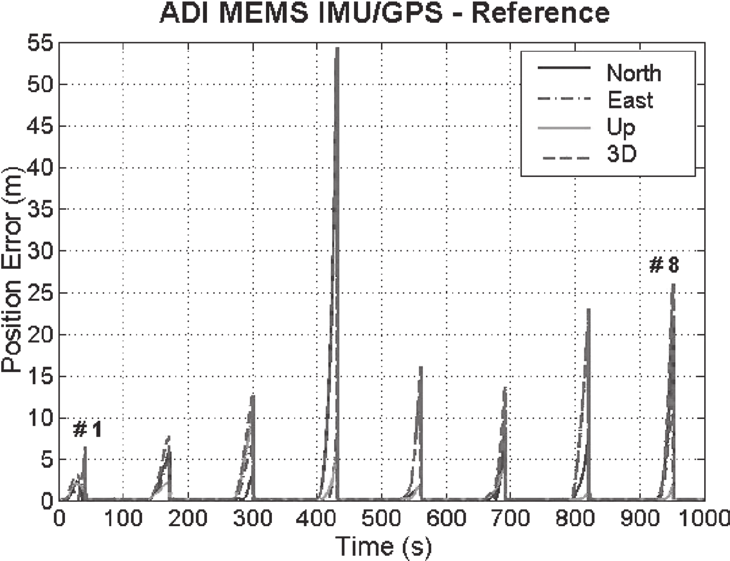
\includegraphics[scale=.2]{2a.png}b)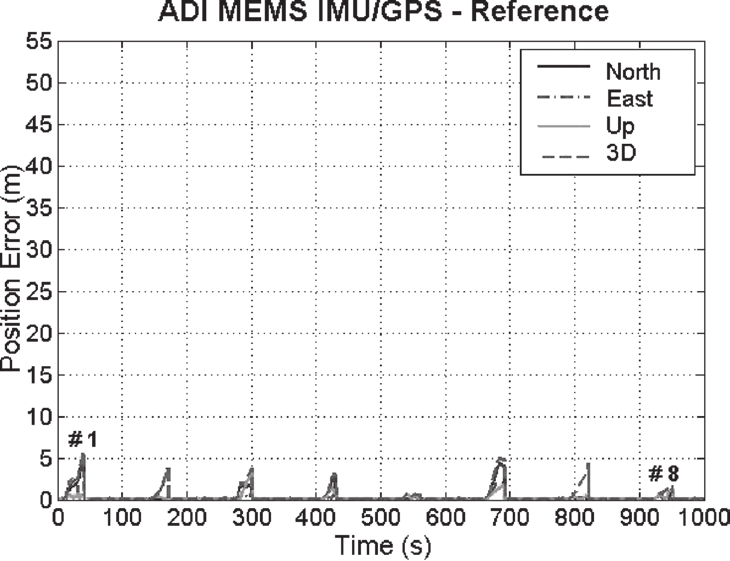
\includegraphics[scale=.2]{2b.png}
%\caption{2 b}
%\end{figure}

\begin{figure}[H]
\begin{tikzpicture}
\centering
  \node[inner sep=0pt] (A) {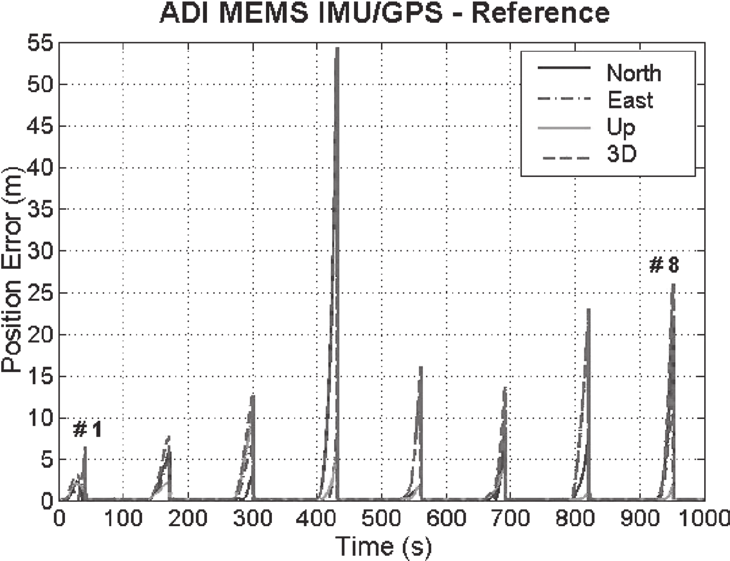
\includegraphics[scale=0.28]{2a.png}\hspace{1cm}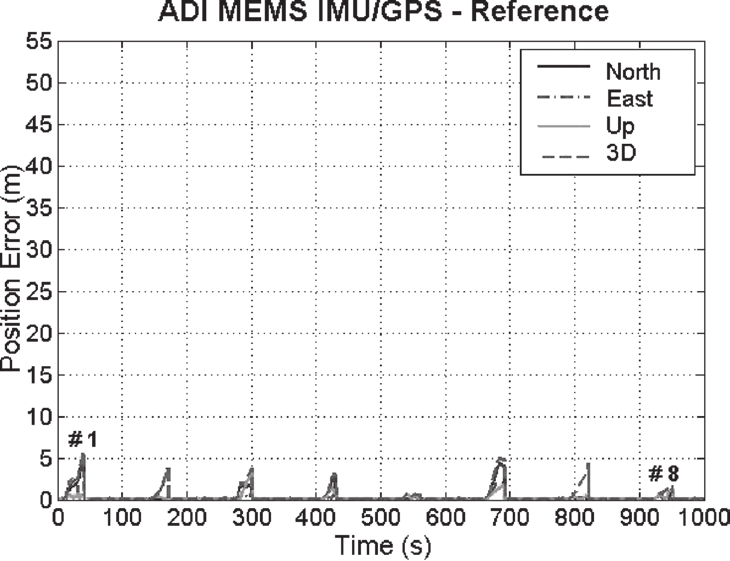
\includegraphics[scale=.28]{2b.png}};
  \node at (-4,-3.4) {$a)$};
  \node at (4,-3.4) {$b)$};
%  \node at (7.7,4.1) {\small #2};
\end{tikzpicture}
\caption{$a)$ Errores de posición durante periodos sin conexión GPS. $b)$ Errores de posición durante periodos sin conexión GPS aplicando actualizaciones auxiliares (imagen tomada de \cite{NAVI:NAVI403}).}
\label{NAVI}
\end{figure}

La integración de IMU’s en los teléfonos móviles es el caso más conocido de la aplicación de estos sensores en la vida cotidiana. 
Sin embargo existen muchas otras aplicaciones, que si bien no son tan masivas y conocidas como el caso de los teléfonos móviles, ayudan a pequeños sectores de la población y de la industria a realizar tareas más eficientemente. 
Como un ejemplo de ello se puede mencionar a los drones, para los cuales este tipo de sensores es indispensable para su correcto funcionamiento \cite{6852167}.

Aún con todas las implementaciones de los sensores de aceleración, todavía existen infinitas posibilidades de aplicación para esta tecnología. 
Por lo que se puede decir que los beneficios directos e indirectos de su uso están aún, en su mayoría, a la espera de que nuevas aplicaciones sean descubiertas y desarrolladas.
 
Muchas de estas aplicaciones ya se están elaborando hoy en día y el espectro de disciplinas en las que podrían aprovecharse sus beneficios es bastante amplio. 
Tal es el ejemplo de los trabajos realizados en \cite{7457644}, donde se hace uso de las IMU’s para activar el motor de bicicletas eléctricas, al detectar mediante estos sensores cuando el usuario conduce en la bicicleta.
También se realiza un análisis del comportamiento de la dinámica de la bicicleta para determinar si el movimiento de esta, corresponde a un desplazamiento común cuando el usuario la va manejando, a un desplazamiento donde el usuario va caminando con ella o a un movimiento accidental del pedal; con el fin de que no se active el motor en estos dos últimos casos.  

\begin{figure}[H]
\centering
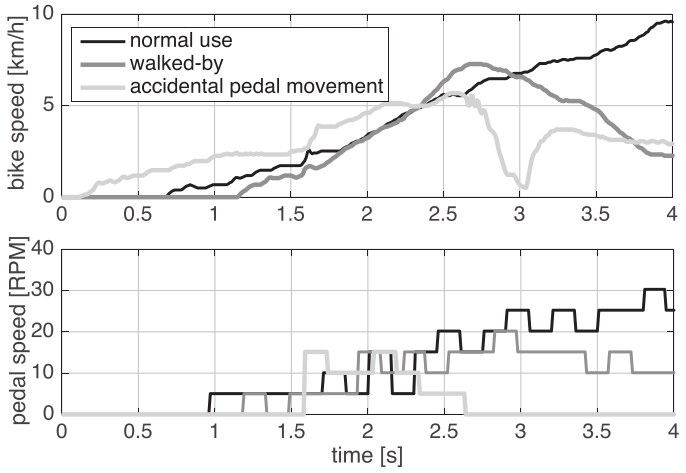
\includegraphics[scale=0.7]{3.png}
\caption{Velocidad de la bicicleta (medida a través de la velocidad del motor) y ritmo del pedal. Se presentan tres eventos diferentes: pedaleo normal, caminar con la bicicleta y movimiento accidental del pedal (imagen tomada de \cite{7457644}).} 
\label{3}
\end{figure}

Otra aplicación interesante de estos dispositivos en medios de transporte es la que se describe en \cite{7072991}. El principal objetivo de este trabajo es la detección de desalineaciones en vías de tren. 
Lo cual se lleva a cabo colocando un sensor inercial dentro de un tren y aplicando la teoría del análisis de Fourier a sus mediciones, con el fin de analizar los espectros de frecuencias y encontrar así posibles desalineaciones. 
Además de que, con este mismo análisis se detecta ruido proveniente del motor y la suspensión del tren. 
Sus beneficios son una mejor identificación de potenciales desalineaciones y su bajo costo en la detección. \\

\begin{figure}[H]
\centering
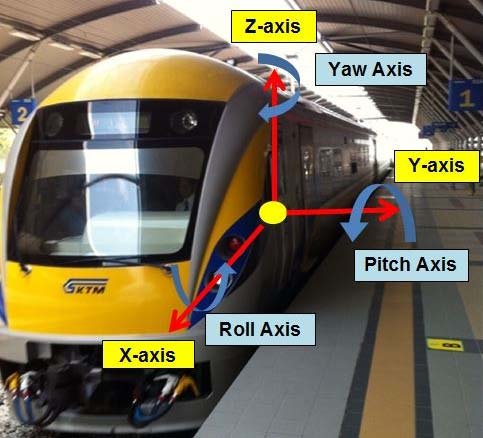
\includegraphics[scale=0.5]{4.png}
\caption{Sistema ejes de los tres ángulos de Euler y ejes de aceleración en el tren (imagen tomada de \cite{7072991}).}
\label{4}
\end{figure}

Análogo al trabajo desarrollado en \cite{7072991} es el proyecto que se expone en \cite{Seraj:2015:SBM:2800835.2800981}, donde en lugar de brindar soluciones para la detección de anomalías producidas en vías férreas, se busca hacer lo equivalente en las autopistas. 
Para esto se hace uso de los sensores integrados en los teléfonos móviles con el fin de recolectar información de la dinámica de un vehículo. 
Esta información es usada para la detección de curvas en el camino, mediante el cálculo del ángulo de desviación del vehículo al dar vuelta. 
Además, con el método implementado se distingue entre distintos eventos de comportamiento de un conductor, al analizar la dinámica del vehículo. 
La detección de anomalías en el camino es lograda al estudiar las características de las curvas, utilizando técnicas como el aprendizaje automático y la Transformada Ondeleta (o Wavelet) Estacionaria.

Otros proyectos orientados a proporcionar soluciones para vehículos, como es el caso del presente trabajo, se enfocan en diferentes cuestiones, las cuales no están necesariamente ligadas a la dinámica del vehículo; tal es el caso de \cite{Quito}.
En este proyecto se tiene el objetivo de identificar y reparar las fuentes de vibración de vehículos pequeños, mediante el uso de la teoría de vibraciones. 
Los autores hacen uso de un analizador (figura \ref{5}), el cual es un aparato que usa la transformada rápida de Fourier para identificar las vibraciones del vehículo; esto se logra colocando el aparato dentro del vehículo y realizando las pruebas correspondientes. 
El dispositivo proporciona información sobre las causas de las vibraciones en vehículos en los que se realizan las pruebas. 
Todo lo anterior con el fin de reducir la molestia de los usuarios por motivos de estas vibraciones, así como a través de este análisis, saber cuando el vehículo se encuentra en mal estado.

\begin{figure}[H]
\centering
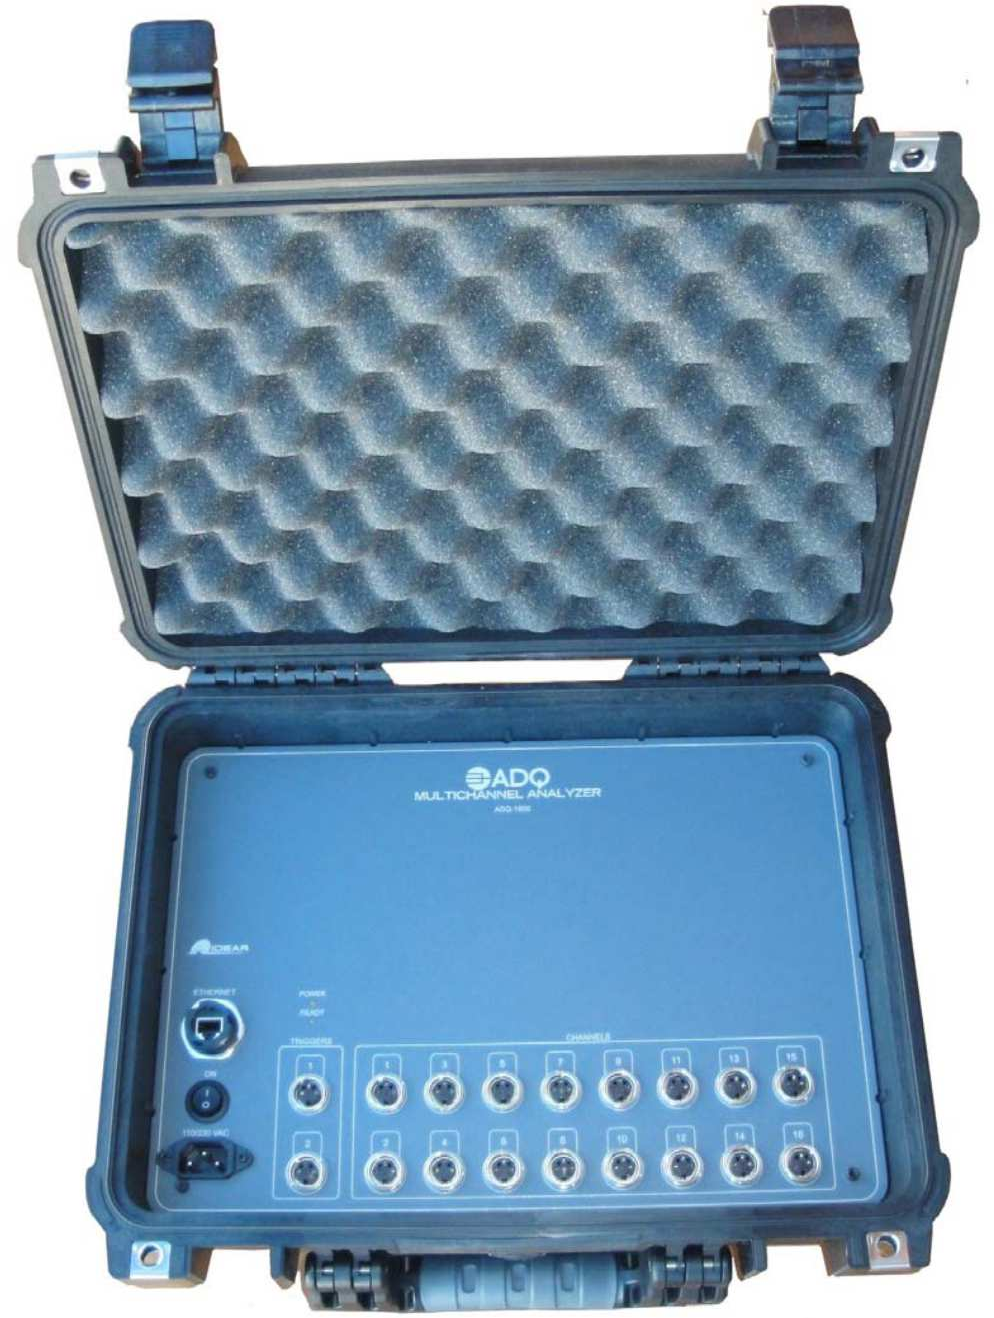
\includegraphics[scale=0.4]{5.png}
\caption{Analizador (imagen tomada de \cite{Quito}).}
\label{5}
\end{figure}

%Además de las metodologías empleadas en este trabajo para la identificación de maniobras anómalas en la conducción de vehículos, existen también otras opciones que ofrecen la solución a esta misma problemática, pero con técnicas muy diferentes a las del análisis espectral o el análisis de la dinámica del vehículo. 
Para dar solución a la problematica descrita en el presente trabajo de tesis existen diferentes técnicas y metodologías.
Una recopilación de varias técnicas para la detección de comportamientos en conductores de automóviles, tales como somnolencia, distracción, ojos cerrados, entre otros, es presentada en \cite{7225158}.
Dentro de estas técnicas, una de las más interesantes es el análisis de imágenes digitales para la detección de los comportamientos mencionados. 
La cual consiste en la colocación de una cámara en el vehículo, de forma tal que, obtenga imágenes del rostro del conductor; para posteriormente, mediante un algoritmo implementado por una computadora, detectar las características de somnolencia, ojos cerrados, etc. 
Otra de las técnicas utilizadas para detectar la fatiga y somnolencia de los conductores es la implementación de análisis psicológicos. 
Con esto se tiene la intención de medir ciertos parámetros físicos y psicológicos, a través de electroencefalogramas y mediciones del ritmo cardiaco del conductor. 
Finalmente, los autores de esta recopilación concluyen diciendo que consideran que cada uno de los métodos que pueden emplearse para la detección de anomalías en la conducción tienen sus pros y contras. 
Por lo que, señalan, la mejor opción es la combinación de varias de estas metodologías.

\begin{figure}[H]
\centering
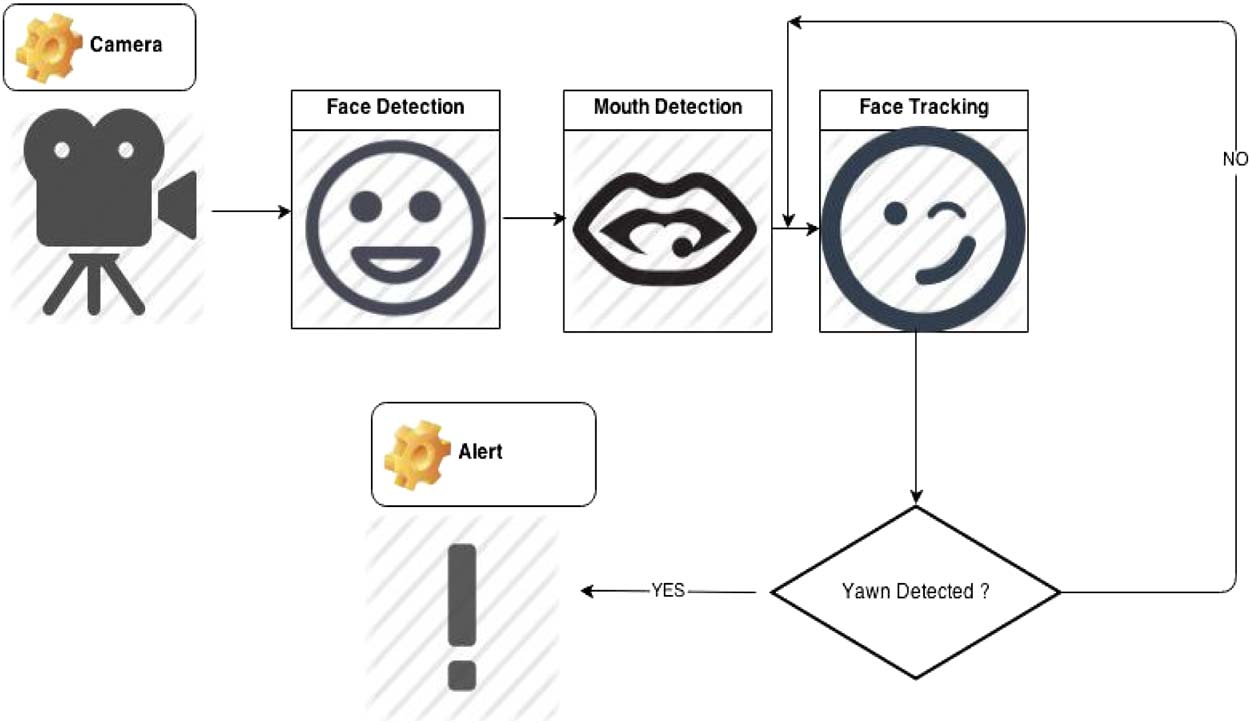
\includegraphics[scale=0.3]{6.png}
\caption{Diagrama de flujo para el análisis de boca y bostezo (imagen tomada de \cite{7225158}).}
\label{6}
\end{figure}


Muchos de los esfuerzos empleados en monitorear la dinámica de un vehículo se centran en el desarrollo de aplicaciones para teléfonos móviles, que ofrezcan información sobre el comportamiento de este a lo largo de alguna trayectoria. 
Uno de los trabajos con estas características es \cite{Valladolid}, donde el principal objetivo de los autores es el análisis de la dinámica del vehículo con fines de detección y prevención de conductas anómalas. 
Su propósito es crear una aplicación móvil que asista al usuario durante la conducción de su vehículo, la cual hace uso de acelerómetros, giroscopios y/o GPS integrados en el teléfono. 
La aplicación que se intenta desarrollar alertará cuando el estilo de conducción sea agresivo mediante sonidos e información en la pantalla del teléfono en tiempo real. 
Buscando siempre que la conducción se haga de manera eficiente.
Mediante el uso del GPS la aplicación mostrará donde se registraron tales eventos de conducción y almacenará la información que se genere durante el trayecto, por ejemplo, datos de aceleración y velocidad en forma gráfica. 
También registrará y mostrará la ruta recorrida mediante la información obtenida por el GPS, señalando los puntos críticos donde se realizaron lo que los autores llaman {\em maniobras agresivas}. 
Se hace un enfoque especial en la detección y posterior aviso de tres eventos de conducción: aceleradas, frenadas y giros. 
La forma de detectar cada uno de los tres diferentes eventos mencionados es a través de umbrales de aceleración y de velocidad angular, por encima de los cuales se considera la realización de alguno de los eventos.

Si bien el uso de teléfonos móviles para el estudio de la dinámica de vehículos tiene un gran potencial, aún existen inconvenientes muy puntuales en el uso de esta tecnología para tales fines.
En \cite{7266726} se busca solucionar el problema de la alineación de los sensores de un teléfono móvil con respecto al vehículo que se pretenda analizar. 
Partiendo de constricciones no holonómicas para la dinámica de un automóvil (como lo es que la velocidad perpendicular a la dirección de movimiento principal del automóvil sea aproximadamente $0$) se busca que la alineación de los sensores quede determinada a lo largo de la navegación del vehículo. 
Actualizándola recursivamente a través del filtro de Kalman, sin la necesidad de una precalibración de los sensores e independientemente de la orientación del teléfono relativa al vehículo.

Otro de los campos de aplicación del análisis de la dinámica de la conducción, aparte de la prevención y alerta de conductas anormales, es la utilización de la información registrada para la deducción de comportamientos del piloto durante la conducción, todo ello con fines legales. 
En \cite{Quito2} se trata de desarrollar un sistema que permita conocer los movimientos y la ruta que ha seguido un vehículo a partir del uso de herramientas tecnológicas como IMU’s y GPS. 
Tal sistema, mostrado en la figura \ref{8}, consiste de una carcasa de metal de $20cm\times 20cm\times 10cm$, la cual contiene el hardware y software necesarios para llevar a cabo los cálculos requeridos para los fines ya mencionados. 
El sistema se conecta a la batería del vehículo, manteniéndolo lo más fijo posible en este para una correcta recopilación de datos. 
Se desea utilizar dicho sistema en la determinación de causas de accidentes de tránsito y localización del vehículo en caso de robo, mediante el análisis de las gráficas de aceleración, velocidad y posición del vehículo que ofrece el dispositivo. 
Para llevar a cabo dicho análisis, en este trabajo los autores realizan pruebas de conducción con el dispositivo a bordo, ejecutando distintas maniobras de prueba con el fin de que los sensores registren su dinámica, tales maniobras se listan a continuación\zsavepos{cont}:
\vspace{8cm}

\begin{textblock*}{\textwidth}(4.7cm,\dimexpr\paperheight-\zposy{cont}sp+5mm)
\begin{itemize}
\item Reposo
\item Conducción normal 
\item Frenado leve 
\item Aceleración rápida 
\item Frenado brusco 
\end{itemize}
\end{textblock*}

\begin{textblock*}{\textwidth}(11.7cm,\dimexpr\paperheight-\zposy{cont}sp+5mm)
\begin{itemize}
\item Camino en mal estado 
\item Aceleración normal 
\item Frenado rápido a fondo
\item Aumento normal de velocidad 
\item Velocidad constante
\end{itemize}
\end{textblock*}

\begin{figure}[H]
\centering
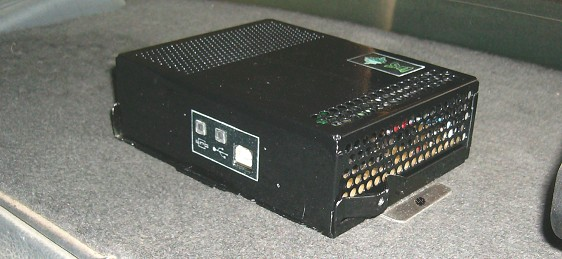
\includegraphics[scale=0.7]{8.png}
\caption{Prototipo instalado en el vehículo (imagen tomada de \cite{Quito2}).}
\label{8}
\end{figure}

Sin embargo, la realización del análisis de las gráficas de aceleración, velocidad y posición generadas en esta prueba solo es de carácter cualitativo.
Ya que los autores únicamente ponen atención a la forma que tienen las diferentes gráficas, para posteriormente deducir si el conductor realizó alguno de los eventos antes mencionados. 

Otra aplicación móvil encaminada a la evaluación del comportamiento de los conductores es la desarrollada en \cite{Paefgen:2012:DBA:2406367.2406412}. 
Donde los autores se basan principalmente en las medidas de aceleración proporcionadas por las IMU’s, así como en información complementaria recibida de otros dispositivos como giroscopios electrónicos y GPS integrados en los teléfonos móviles. 
Esto para detectar lo que ellos llaman eventos críticos de conducción, los cuales se listan a continuación:

\begin{itemize}
\item Aceleración
\item Frenada
\item Vuelta a la izquierda
\item Vuelta a la derecha
\end{itemize}

La detección de estos eventos está basada en la superación de diferentes umbrales de aceleración, correspondientes a cada evento. 
Con la información recabada por el teléfono móvil se pretende dar la correspondiente retroalimentación a los conductores a través de la aplicación; brindándoles información sobre la forma en la que condujeron sus recorridos y añadiéndola a un perfil generado por esta aplicación. 
Cabe mencionar que en este estudio se toma en cuenta el tipo de carretera como factor a considerar en la obtención de datos, característica que no se toma en cuenta muchos otros trabajos relacionados.
Los autores justifican que una aplicación móvil es una mejor opción que una {\em caja negra} (como la que se desarrolla en \cite{Quito2}), ya que, según ellos, tiene una mejor interactividad y permite al usuario tener un mejor acceso y manejo de su información; todo ello con vías a mejorar su comportamiento en la conducción.
Además, mediante el uso de la aplicación se pueden establecer redes sociales que contribuyan a mejorar la seguridad en el tráfico de vehículos.

En \cite{vaiana2014driving} se señala que la seguridad en el tráfico y la eficiencia en el gasto de energía de los vehículos están estrictamente ligados al comportamiento del conductor. 
En este artículo se explica el desarrollo de una aplicación para teléfonos móviles, que pueda evaluar el grado de seguridad que los conductores mantienen al conducir; esto por medio de mediciones de aceleración longitudinal y lateral. 
Para ello se realizan varias pruebas con distintos conductores y vehículos. 
La forma en que se detecta si se está realizando un correcto o incorrecto estilo de conducción es mediante el estudio de las gráficas de aceleración obtenidas, donde se tienen áreas designadas para diferentes formas de conducir. 
La evaluación de la forma de conducir dependerá de la zona de la gráfica donde se registren los datos de aceleraciones cuando el vehículo esté en movimiento. 
Un ejemplo de los registros de datos correspondientes a dos formas de conducción diferentes se da en la figura \ref{10(2)}.

\begin{figure}[H]
\centering
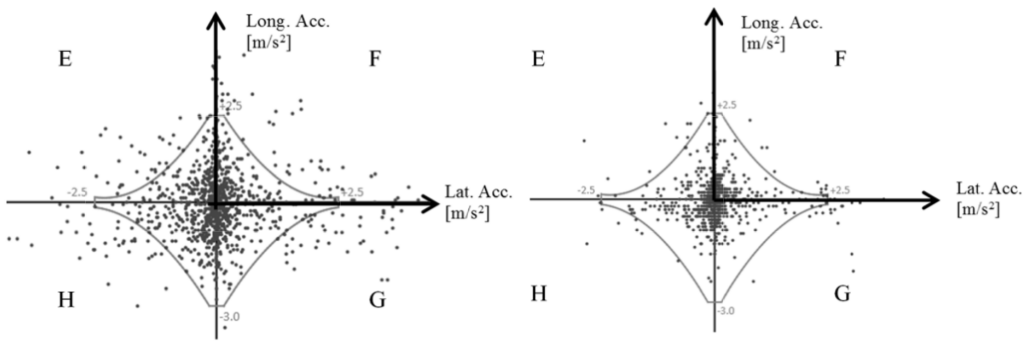
\includegraphics[scale=0.5]{10(2).png}
\caption{Distribución de puntos en el Diagrama de Estilo de Conducción para un conductor agresivo (izquierda) y uno conservador (derecha) (imagen tomada de \cite{vaiana2014driving}).}
\label{10(2)}
\end{figure}

En \cite{wu2013driving} se hace el prototipo de un dispositivo para el registro de eventos de conducción basado en el comportamiento al conducir, mediante el uso de herramientas como acelerómetros, cámaras y GPS.
Este dispositivo provee información acerca de siete comportamientos al conducir: conducción normal, aceleración, desaceleración, cambio al carril izquierdo o derecho, conducción en zigzag y aproximación al vehículo de enfrente.
El prototipo consiste en un arreglo de los componentes mencionados en forma de caja. 
Los resultados experimentales de este trabajo logran un promedio de $95\%$ de detección para el reconocimiento de comportamientos al conducir.

El trabajo realizado en \cite{6856461} trata sobre del desarrollo de una aplicación para teléfonos móviles, la cual detecta comportamientos de distracción a la hora de conducir, brindando las correspondientes observaciones a los conductores y alertándolos en caso de que su modo de conducir sea inseguro. 
La finalidad del desarrollo de esta aplicación es evitar accidentes automovilísticos, así como fomentar las prácticas de conducción seguras entre los usuarios. 
Las herramientas utilizadas para tales fines son sensores inerciales, GPS, cámaras y micrófonos. 
El proceso para lograr la detección comienza colocando el teléfono móvil justo debajo del espejo retrovisor, con la cámara apuntando hacia la carretera. 
Una vez hecho esto, la aplicación utiliza técnicas de reconocimiento de patrones con el fin de detectar los comportamientos de distracción más comunes en la conducción; tales como, cambiar de carril sin encender las luces intermitentes o la incapacidad del conductor para mantener el vehículo centrado en el carril correspondiente. 
Todo ello se logra al hacer uso de la información obtenida por la cámara y los sensores del teléfono, identificando automáticamente las líneas delimitadoras de los carriles y analizando el comportamiento del vehículo respecto a estas. 
La superación de umbrales de aceleración es otro de los factores importantes para la detección de tales comportamientos.

\begin{figure}[H]
\centering
\begin{tikzpicture}
  \node{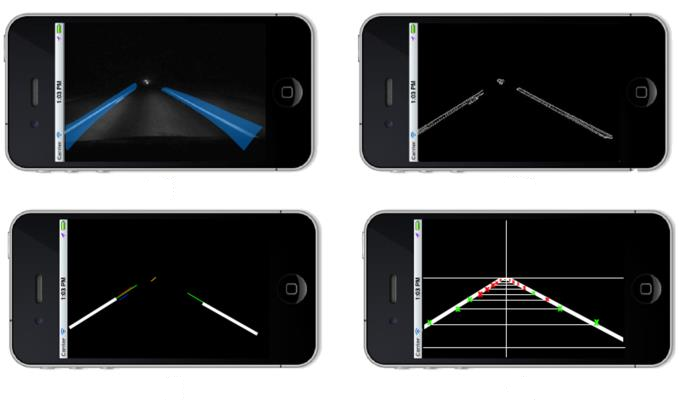
\includegraphics[scale=0.8]{12(2).png}};
  \node at (-3.6,.2) {$a)$};
  \node at (4,.2) {$b)$};
  \node at (-3.6,-4) {$c)$};
  \node at (4,-4) {$d)$};
\end{tikzpicture}
\caption{Proceso de detección de líneas en la noche: $a)$ Regiones de interés en escala de grises. $b)$ Límites de la carretera. $c)$ Líneas segmentadas y continuas. $d)$ Indicador de mediciones y modelado de camino (imagen tomada de \cite{6856461}).}
\label{12(2)}
\end{figure}

En \cite{6728289} se desarrolla un método que busca crear perfiles de comportamiento de conductores. 
También se trata de identificar eventos de conducción peligrosos, mediante el análisis de información recopilada por sensores en un vehículo. 
Para ello se recurre a la utilización de diferentes dispositivos incluidos en los teléfonos móviles: acelerómetro, GPS y magnetómetro. 
La información registrada al finalizar un recorrido común a bordo de un vehículo se envía a un servidor, en el cual se analizan los diferentes comportamientos de los conductores. 
Cada perfil de conducción se construye en base a 12 variables, medidas a lo largo de cada recorrido. 
Las cuales son utilizadas en un sistema de lógica difusa como el que se muestra en la tabla \ref{14(2)}, compuesto por 18 reglas, donde el resultado de cada una informa cual fue el tipo de conducción realizado de entre tres posibilidades: moderado, normal y agresivo. 

\begin{table}[H]
\centering
\begin{tabular}{c|c|c}
\hline \hline
\multicolumn{3}{p{10cm}}{\centering \bf Reglas de inferencia} \\ % p{ancho de texto}
\hline \hline 
No. & IF & THEN \\ \hline
1 & $OS_T=L\ \text{\fontfamily{qcr}\selectfont AND}\ OS_A=L\ \text{\fontfamily{qcr}\selectfont AND}\ OS_P=L$ & $NOR$\\ 
2 & $OS_T=M\ \text{\fontfamily{qcr}\selectfont AND}\ OS_A=M\ \text{\fontfamily{qcr}\selectfont AND}\ OS_P=M$ & $MOD$\\
3 & $OS_T=H\ \text{\fontfamily{qcr}\selectfont AND}\ OS_A=H\ \text{\fontfamily{qcr}\selectfont AND}\ OS_P=H$ & $AGG$\\
4 & $(SA_M=L\ \text{\fontfamily{qcr}\selectfont OR}\ SA_M=M)\ \text{\fontfamily{qcr}\selectfont AND}\ SA_A=L$ & $NOR$\\
5 & $(SA_M=M\ \text{\fontfamily{qcr}\selectfont OR}\ SA_M=H)\ \text{\fontfamily{qcr}\selectfont AND}\ SA_A=L$ & $MOD$\\
6 & $(SA_A=M\ \text{\fontfamily{qcr}\selectfont OR}\ SA_A=H)\ \text{\fontfamily{qcr}\selectfont AND}\ SA_M=H$ & $AGG$\\
7 & $(GA_M=L\ \text{\fontfamily{qcr}\selectfont OR}\ GA_M=M)\ \text{\fontfamily{qcr}\selectfont AND}\ GA_A=L$ & $NOR$\\
8 & $(GA_M=M\ \text{\fontfamily{qcr}\selectfont OR}\ GA_M=H)\ \text{\fontfamily{qcr}\selectfont AND}\ GA_A=L$ & $MOD$\\
9 & $(GA_A=M\ \text{\fontfamily{qcr}\selectfont OR}\ GA_A=H)\ \text{\fontfamily{qcr}\selectfont AND}\ GA_M=H$ & $AGG$\\
10 & $GA_P=L\ \text{\fontfamily{qcr}\selectfont AND}\ GA_N=L$ & $NOR$\\
11 & $GA_P=M\ \text{\fontfamily{qcr}\selectfont AND}\ GA_N=M$ & $MOD$\\
12 & $GA_P=H\ \text{\fontfamily{qcr}\selectfont AND}\ GA_N=H$ & $AGG$\\
13 & $(BR_M=L\ \text{\fontfamily{qcr}\selectfont AND}\ BR_M=M)\ \text{\fontfamily{qcr}\selectfont AND}\ BR_A=L$ & $NOR$\\
14 & $(BR_M=M\ \text{\fontfamily{qcr}\selectfont AND}\ BR_M=H)\ \text{\fontfamily{qcr}\selectfont AND}\ BR_A=L$ & $MOD$\\
15 & $(BR_A=M\ \text{\fontfamily{qcr}\selectfont AND}\ BR_A=H)\ \text{\fontfamily{qcr}\selectfont AND}\ BR_M=H$ & $AGG$\\
16 & $BR_P=L$ & $NOR$ \\
17 & $BR_P=M$ & $MOD$ \\
18 & $BR_P=H$ & $AGG$ \\
\hline \hline
\end{tabular}
\caption{Lista de reglas de inferencia (tabla tomada de \cite{6728289}).}
\label{14(2)}
\end{table}

La forma en que los autores evalúan el comportamiento del conductor es asignándole una puntuación a cada una de las salidas. 
Las cuales son sometidas a una serie de operaciones, dando como resultado una puntuación final entre $0$ y $100$, siendo $0$ la mejor y $100$ la peor.

Usando métodos similares a los explicados en \cite{6728289}, tales como sistemas de lógica difusa, los autores de \cite{7014406} desarrollan una plataforma que utiliza el acelerómetro, GPS, magnetómetro y sensor de gravedad incluidos en los teléfonos móviles. Esto con el propósito de registrar información durante el trayecto de un vehículo, la cual servirá para crear un perfil de conducción para cada usuario. 
También buscan ofrecer información sobre eventos de riesgo individual de los conductores, así como de la rapidez y manejo ecológico del vehículo. 
Una de las características que distingue a este trabajo de otros similares es el uso de información sobre condiciones climáticas como factor para determinar los eventos de riesgo. 
Dentro de los eventos de riesgo, los autores intentan detectar exceso de velocidad, aceleración, frenado y direccionamiento. 
Mediante notificaciones sonoras y gráficas en el teléfono móvil se alerta al usuario sobre la ocurrencia de alguno de estos eventos.

En \cite{7338354} se tiene el propósito de realizar un monitoreo detallado de los comportamientos anormales en la conducción de automóviles, dando la retroalimentación correspondiente a los conductores; para lo cual se realiza una recopilación de datos de conducción en ambientes reales durante seis meses. 
Los autores identifican seis tipos de comportamientos anómalos de conducción: movimiento trenzado, desviación, deslizamiento, movimiento en U rápido, giro de amplio radio y frenado repentino.
Estos son detectados al aplicar técnicas de aprendizaje automático a los datos obtenidos, para ello se establecen 16 características representativas que pueden identificar a cada uno de los seis comportamientos de conducción. 
Tales características constan de diferentes parámetros de aceleración, orientación, tiempo de ejecución de los eventos, entre otros; los cuales son determinados a partir de las mediciones de los sensores. 
Complementariamente, se estima el impacto de diferentes factores sobre el desempeño de la plataforma, tales como condiciones de tráfico, tipo de carretera, lugar de colocación del teléfono, entre otros.

En \cite{Hong:2014:SSP:2611222.2557321} se propone la implementación de una plataforma de medición, con la cual se pretende realizar una valoración y evaluación automática del estilo de conducción. 
La plataforma hace uso de los sensores incluidos en teléfonos móviles, dispositivos para el diagnóstico del vehículo y técnicas de aprendizaje automático. 
La metodología empleada para la evaluación requiere de la información de un cierto número de características relativas a la conducción, las cuales se encuentran en la diversa información recolectada. 
Dicha información está compuesta por datos de velocidad, aceleración, desaceleración, revoluciones por minuto del motor, posición del acelerador y dirección del movimiento de las ruedas. 
Los autores tienen como objetivo que en el futuro se puedan identificar estilos de conducción agresivos en tiempo real, así como proveer la retroalimentación pertinente al conductor, con el fin de mejorar el estilo de conducción de los usuarios. 

Haciendo un resumen de los trabajos presentados en este capítulo, se puede destacar la gran cantidad de aplicaciones para teléfonos móviles, desarrolladas con fines de prevención de conductas incorrectas en la conducción.
Lo cual es debido principalmente a la masificación y disminución en los costos de dispositivos como las IMU's.
Tal accesibilidad en estos dispositivos también ha dado lugar al desarrollo de soluciones en diferentes ámbitos de la conducción de vehículos, las cuales no están necesariamente enfocadas en automóviles, sino en vehículos como bicicletas o trenes.

Las metodologías empleadas para la detección de diferentes conductas en los pilotos, así como de movimientos anormales en los distintos medios de transporte analizados son muy variadas; van desde análisis en la dinámica de los vehículos en tiempo real, hasta el uso de electroencefalogramas para estudios del comportamiento de los usuarios a la hora de conducir.
Sin embargo, en la investigación realizada de los trabajos relacionados, se encontró que estos utilizan mayoritariamente el estudio de la dinámica a diferentes niveles, junto con umbrales de aceleración y/o velocidad predefinidos; o bien, sistemas muy sofisticados con multiples sensores para la determinación de conducciones anómalas.
La propuesta que se realiza en este trabajo difiere de las presedentes en que no se basa en el estudio de la dinámica propia del vehículo, además de que solo requiere de un dispositivo IMU como sensor.
En el siguiente capítulo se detallarán las bases teóricas y componentes de hardware utilizados para este trabajo.

% !TEX encoding = UTF-8 Unicode
\chapter{Marco teórico}
\label{chap:marco_teorico}
%
%
En este capítulo se definirán de manera formal los elementos que componen el problema propuesto, así como las herramientas útiles para resolverlo.
De igual manera, se describirán las características de las instancias específicas que se abordarán y se hará un análisis de la complejidad de su espacio de búsqueda asociado.
%
%
\section{Definiciones y consideraciones del problema}
\label{sec:definiciones_y_consideraciones}
%
%
Antes de establecer las bases teóricas del problema que se desea abordar, se describirán el contexto y las condiciones iniciales que lo caracterizan.
De esta manera, los elementos necesarios para poder definir el problema planteado son: 
%
\begin{itemize}
	\item Un espacio plano y limitado sobre el cual se pueden colocar objetos.
	\item Un conjunto\footnote{Debido a cuestiones prácticas, se utilizará la palabra \textsl{conjunto}, aunque técnicamente lo correcto sería \textsl{multiconjunto}, ya que en los objetos a acomodar están permitidas las repeticiones.} de objetos, los cuales tienen asociados individualmente un conjunto de atributos y una clase, la cual está definida a partir de los primeros.
	\item Una vecindad asociada a cada objeto colocado en el espacio.
	\item Un conjunto de formas de sujeción asociadas a cada clase de objeto, definidas en función de su geometría, las cuales pueden ser utilizables o no dependiendo del estado de la vecindad del objeto.
	\item Un conjunto de acciones, aplicables a cada objeto.
\end{itemize}
%
A continuación se definen de forma detallada cada uno de los componentes anteriores y posteriormente se hará una asignación de valores para tratar un problema en particular, esto con el objetivo de demostrar el funcionamiento del algoritmo propuesto.

Sea $E$ un espacio discreto (malla) de $n\times m$ localidades o celdas como el que se muestra en la Figura \ref{fig:malla}.
Cada una de las celdas de $E$ será representada por $e_{ij}$, con $1 \leq i \leq n$ y $1 \leq j \leq m$.
%
\begin{figure}[H]
	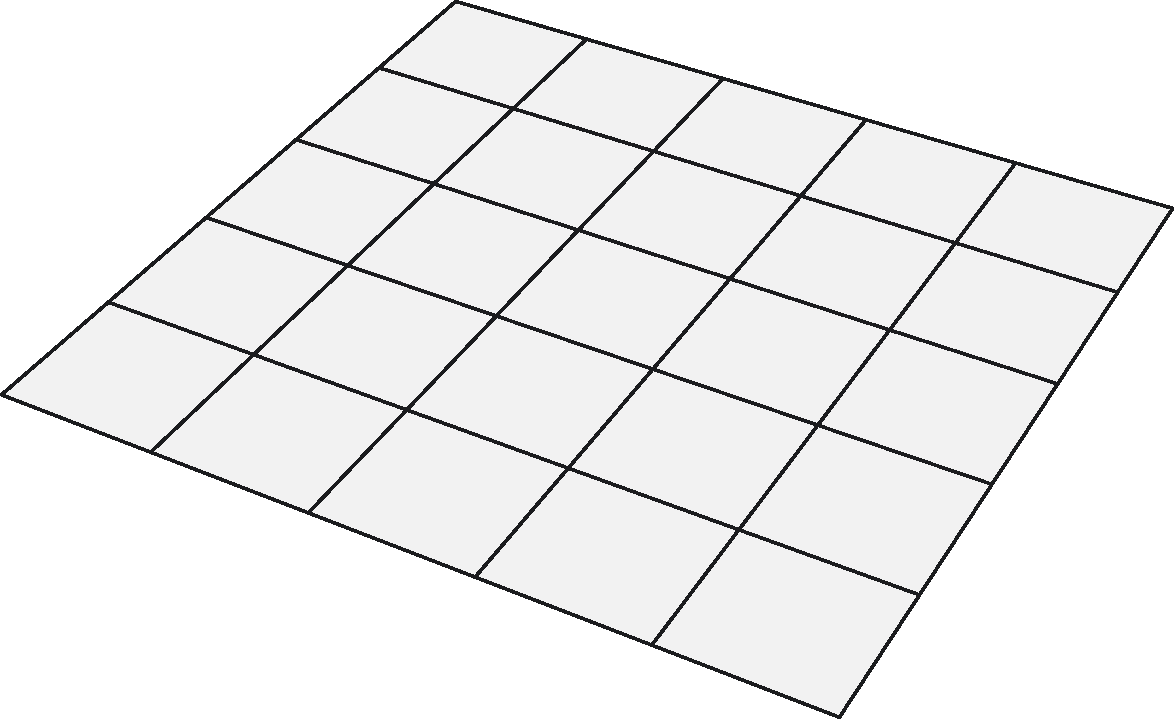
\includegraphics[width=0.6\textwidth]{malla}%
	\caption{Espacio discretizado de dos dimensiones.}%
	\label{fig:malla}%
\end{figure}
%
Se desea colocar en el espacio $E$ un conjunto de objetos particulares.
Sea:
%
\begin{equation}
\label{eq:objetos}
O = \{ o_1, o_2, \ldots, o_N \}
\end{equation}
%
el conjunto de $N$ objetos disponibles para colocar en las celdas de $E$, donde $o_k$ representa el $k$-ésimo objeto, con $1 \leq k \leq N$.

Sea:
%
\begin{equation}
\label{eq:atributos}
A = \{ a_1, a_2, \ldots, a_{N_A} \}
\end{equation}
%
el conjunto de atributos que puede tener un objeto y que son de utilidad para resolver el problema definido; por ejemplo: el tamaño, el color, la forma, etc.
Siendo $N_A$ el número máximo de atributos, y sea:
%
\begin{equation}
\label{eq:atributos_objeto}
A_k = \left\{ a_{k, 1}, a_{k, 2}, \ldots, a_{k, N_A} \right\}
\end{equation}
%
el conjunto de atributos asociado a un objeto $o_k$.
De esta manera, mientras que $a_{1}$ representa el nombre de un atributo en particular, por ejemplo \textit{color}; $a_{k, 1}$ corresponde al valor o instancia de dicho atributo para el objeto $o_k$, por ejemplo, \textit{verde}.

La condición necesaria y suficiente para que dos objetos se consideren diferentes es que difieran en al menos el valor de uno de sus atributos.

El conjunto general de atributos $A$ se ha definido para fomentar que los objetos compartan la mayor cantidad de atributos posible, así como que estos atributos sean lo más generales posible, para que de esta manera el problema pueda ser resuelto con la mínima cantidad de atributos necesarios, reduciendo de esta forma su complejidad.

Así, se motiva a encontrar la representación más simple de los objetos (e.g. mediante su caja contenedora) que satisfaga las necesidades de manipulación del problema.
Por ejemplo, si para los fines de manipulación del problema es suficiente que un objeto particular con geometría compleja pueda ser tratado como un cubo u otra figura de geometría más simple, esto ayudará a simplificar la búsqueda de la configuración óptima de objetos, así como la definición de las formas en que estos pueden ser sujetados.

Sea:
%
\begin{equation}
\label{eq:clases}
C = \{ C_1, C_2, \ldots, C_{N_C} \}
\end{equation}
%
el conjunto de clases a las que pertenecen los objetos de $O$, donde $N_C$ es el número máximo de clases.

Cada clase $C_K$, con $1 \leq K \leq N_C$, representa un conjunto de atributos $A_k$ distinto.
De esta manera, si los conjuntos de atributos $A_1$, $A_2$ y $A_3$ correspondientes a los objetos $o_1$, $o_2$ y $o_3$, son iguales, se considera que todos ellos pertenecen a la misma clase, aunque en la realidad puedan diferir en algún atributo no considerado en su conjunto de atributos.
En particular, el trabajar con un número elevado de clases de objetos no es, por el momento, de interés en el presente trabajo, ni el objetivo de la definición de clases previa, sino lo contrario: crear un conjunto de clases de atributos que sean lo más similares entre sí para reducir la complejidad del problema.

La manera en que se definen estas clases ayudará a simplificar el problema, ya que permite, cuando sea posible, que objetos con determinadas características en común (sin que necesariamente sean iguales en la realidad) sean identificados como de la misma clase y manejados de forma similar o igual; por ejemplo, en lo que a su sujeción se refiere.

Sea:
%
\begin{equation}
\label{eq:vecindad}
V_{ij} = \{ v_1, v_2, \ldots, v_{N_V} \}
\end{equation}
%
el estado de la vecindad con respecto a la celda $e_{ij}$; donde $v_{k_V}$ es el estado individual de una celda vecina, con $1 \leq k_V \leq N_V$, donde $N_V$ es el número de celdas vecinas (tamaño de la vecindad) a considerar.

El número de celdas vecinas $N_V$ y su localización, dependerán del tipo de problema que se vaya a tratar.
Según la definición del espacio discretizado $E$, algunas de las vecindades posibles se pueden conformar, por ejemplo, de 4, 8 o 24 elementos, como se muestra a continuación:
%
\begin{figure}[H]
	\begin{subfigure}[b]{0.45\textwidth}
		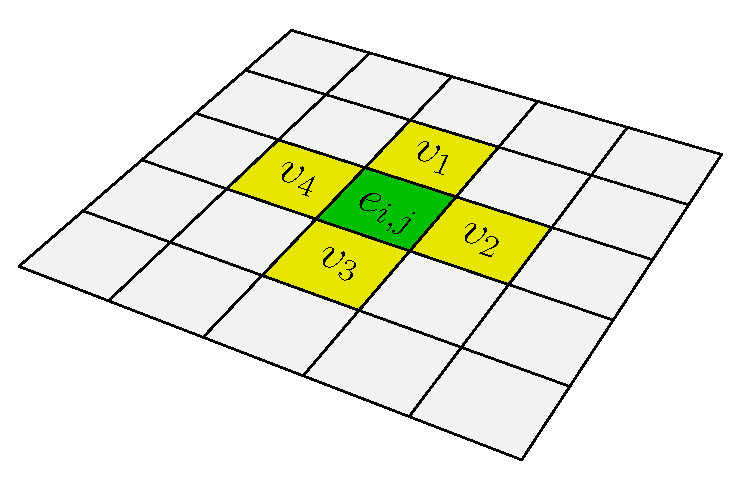
\includegraphics[width=\textwidth]{vecindad}%
		%\caption{}%
		\label{subfig:4_vecinos}%
	\end{subfigure}%
	%
	\hspace{1cm}
	%
	\begin{subfigure}[b]{0.45\textwidth}
		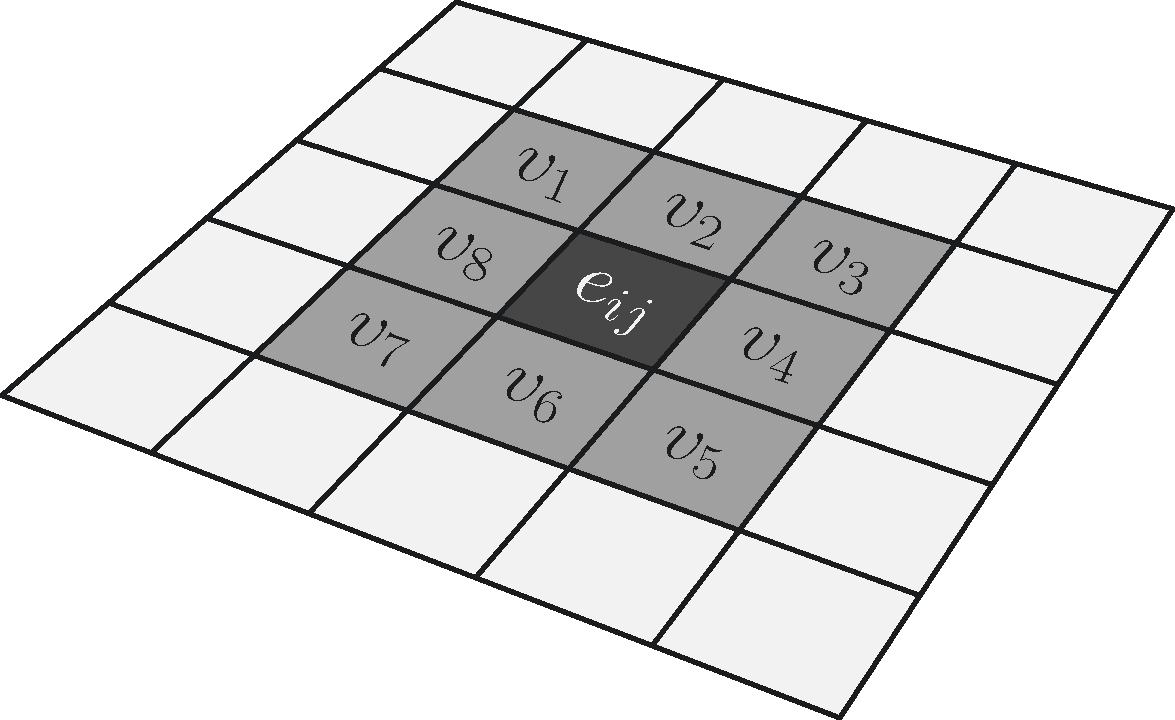
\includegraphics[width=\textwidth]{vecindad_alternativa_1}%
		%\caption{}%
		\label{subfig:8_vecinos}%
	\end{subfigure}%

	\begin{subfigure}[b]{0.45\textwidth}
		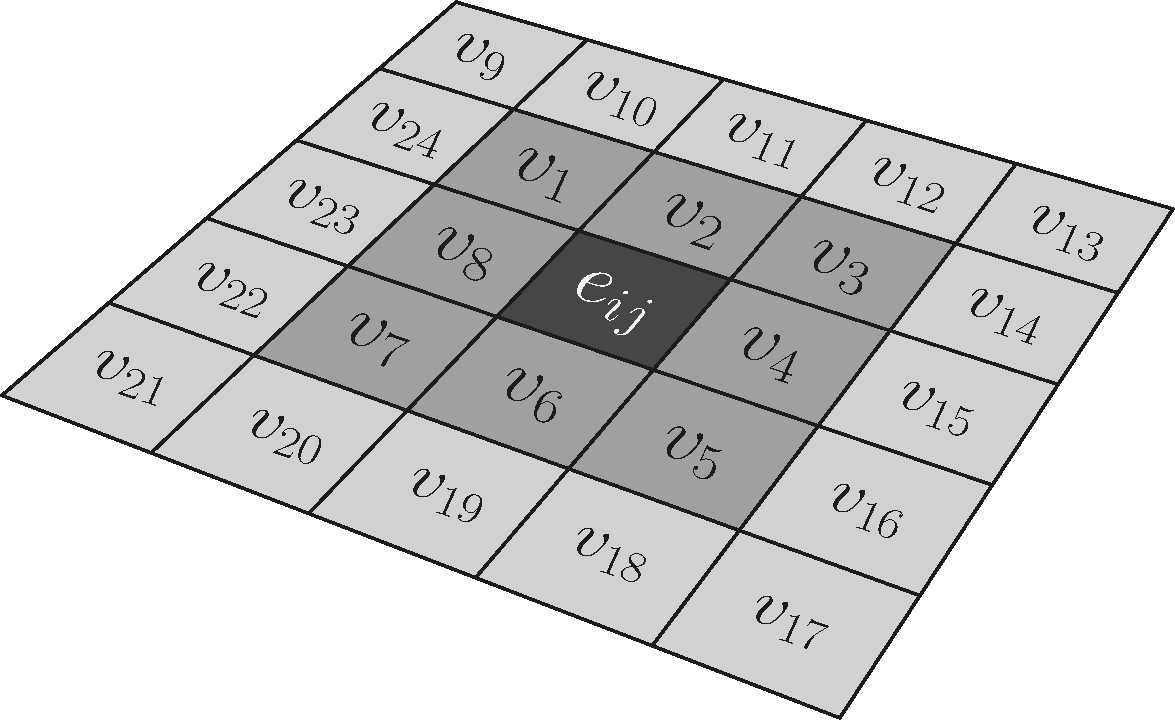
\includegraphics[width=\textwidth]{vecindad_alternativa_2}%
		%\caption{}%
		\label{subfig:24_vecinos}%
	\end{subfigure}%
	%
	\caption{Ejemplos de vecindades de 4, 8 y 24 vecinos.}%
	\label{fig:vecindades}%
\end{figure}
%
De esta manera, el estado de la vecindad $V_{ij}$ consiste en el listado de los estados individuales de las celdas consideradas como vecinas a $e_{ij}$, donde cada uno de estos puede ser: contener un objeto de $O$ o no contener ningún objeto (celda vacía), esto es: $v_k \rightarrow O \cup \{ \boxslash \}$.

Sea:
%
\begin{equation}
\label{eq:sujecion}
S = \left\{s_1, s_2, \ldots, s_{N_S}\right\}
\end{equation}
%
el conjunto de todas las formas de sujeción de todas las clases de objetos de $O$.
Una forma de sujeción se define como un conjunto de puntos, curvas y/o superficies de contacto de un objeto particular, a partir de las cuales este se puede sujetar.
De esta manera, una forma de sujeción $s_{k_S}$ podría ser, por ejemplo, la que especifique el conjunto de puntos de contacto de un objeto particular, sobre los cuales se tendría que ejercer presión, succión o algún otro acto (dependiendo del manipulador utilizado) para sujetarlo.

La definición de las formas de sujeción depende directamente del tipo de manipulador que se vaya a utilizar, de las características del objeto que se vaya a manipular, entre otros factores.
Cabe señalar que, en general, las formas de sujeción aplicables a un objeto determinado, no tienen que serlo para otro objeto, debido principalmente a las variaciones en la geometría de estos, pero, en general, puede ser conveniente que, además de que la cantidad de formas de sujeción para cada objeto sean mínimas, estas sean iguales o lo más similares posible (como las utilizadas en el presente trabajo), con el objetivo de reducir la complejidad del problema.
Es por ello que, de forma similar a la definición de los conjuntos de atributos, se define un conjunto general $S$ de formas de sujeción, ya que tanto el preferir geometrías simples para representar las distintas clases de objetos, como el definir formas de sujeción comunes a estas representaciones, simplificará el problema en la medida de lo posible.

Sea:
%
\begin{equation}
\label{eq:sujecion_objeto}
S_K = \left\{s_{K, 1}, s_{K, 2}, \ldots, s_{K, N_S}\right\}
\end{equation}
%
el conjunto de formas de sujeción asociadas a los objetos de la clase $C_K$, donde cada $s_{K, k_S}$ puede ser restringida en función de la vecindad asociada al objeto en cuestión.

Para el problema particular que se tratará en este trabajo, detallado en la siguiente sección, se han definido formas de sujeción de manera bastante sencilla y muy general, sin embargo, estas formas pueden ser tan complejas como se requiera para una tarea en particular.

Finalmente, sea:
%
\begin{equation}
\label{eq:acciones}
W = \{w_1, w_2, \ldots, w_{N_W}\}
\end{equation}
%
el conjunto de acciones que se pueden aplicar a un objeto particular, ya sea dentro del espacio $E$ o fuera de este, tal que modifican el estado de $E$.
Estas acciones se definen según las características del problema a tratar; las cuales pueden ser, por ejemplo: quitar un objeto de $E$; añadir un objeto a $E$, cambiar su posición dentro de $E$, cambiar su orientación, etc.

Sea $t_{ij}$ la variable que cuantifica el número de acciones necesarias para tomar el objeto en $e_{ij}$.
Esto es, $t_{ij}-1$ es el número de objetos-obstáculo que impiden tomar el objeto de interés en $e_{ij}$.
Por lo tanto, $t_{ij}$ también se define como el costo asociado para tomar un objeto.

La forma de calcular $t_{ij}$ está en función de la vecindad del objeto en $e_{ij}$ y, recursivamente, de la vecindad de sus vecinos hasta llegar a una condición de paro; lo cual se presenta en la Sección \ref{subsec:costo}.

Asimismo, se define el costo global $T$ de un acomodo de objetos como la suma de los costos individuales $t_{ij}$:
%
\begin{equation}
\label{eq:costo_global}
	T = \sum_{i,\hspace{1pt} j}\ t_{ij}
\end{equation}
%
El objetivo principal en este trabajo es encontrar una configuración o acomodo de todos los objetos de $O$ en el espacio $E$; de forma que el número de acciones $t$ o cambios de estado promedio para acceder y finalmente tomar a cada uno de los objetos sea mínimo.
En esta etapa del proyecto, se considera que las acciones que se pueden realizar para acceder a un objeto únicamente consisten en quitar un objeto de $E$.
La acción correspondiente al cambio de posición dentro de $E$ de un objeto, considerado como obstáculo, no se considera, pero se puede añadir en una posterior extensión del proyecto.

Adicionalmente, tomando en cuenta la posición de un objeto $o_k$ en la malla, su clase $C_K$ y el estado de su vecindad $V_{ij}$, se considera que, el conjunto de formas de sujeción asociadas $S_K$ puede variar, llegando en ocasiones a restringirse de forma parcial o total las formas en que este se puede sujetar.
%
%
\section{Especificaciones del problema a tratar}
\label{sec:especificaciones}
%
%
Para acotar el problema, en esta sección se definirán instancias específicas de los conjuntos enunciados en la sección anterior, así como de las variables asociadas a ellos.
Los detalles del problema particular a tratar se dan a continuación.
%
%
\subsection{Espacio de trabajo}
\label{subsec:espacio_trabajo}
%
%
Para evaluar el rendimiento del algoritmo propuesto se utilizaron diferentes tamaños de malla.
La Figura \ref{fig:ejes_malla} muestra un ejemplo de la configuración de ejes utilizada para ubicar cada celda $e_{ij}$ en una malla de $5\times 5$.
En las figuras y expresiones matemáticas utilizadas en este documento, la configuración de ejes se mantiene, o bien, es la que más se aproxima a la que muestra la Figura \ref{fig:ejes_malla}.
%
\begin{figure}[H]
	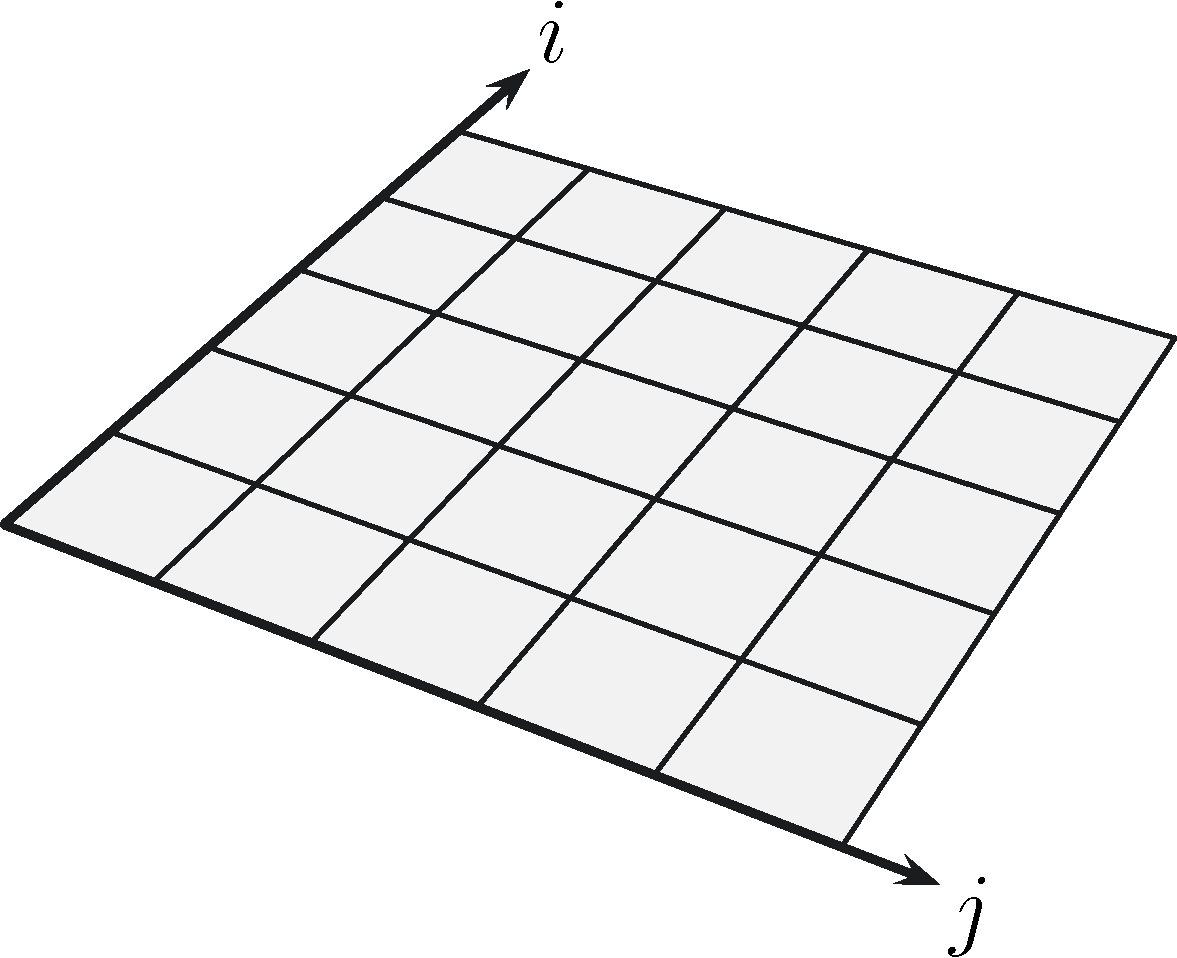
\includegraphics[width=0.6\textwidth]{ejes_malla}%
	\caption{Configuración de los ejes para la ubicación de las celdas mediante la notación $e_{ij}$.}%
	\label{fig:ejes_malla}%
\end{figure}
%
Es importante hacer notar que, el tamaño o discretización de las celdas de $E$ solo permite colocar en cualquiera de estas un y solo un objeto, de cualquier clase.
%
%
\subsection{Características de los objetos}
\label{subsec:objetos}
%
%
El conjunto de objetos $O$ consiste, en esta fase inicial del proyecto, de objetos pertenecientes a una de dos clases posibles, siendo la clase $C_1$ un cubo y la clase $C_2$ un prisma rectangular, ambos objetos de base idéntica correspondiente a una cara del cubo (Figura \ref{fig:objetos}).
La altura del prisma es igual al doble de la longitud de un lado de un cubo.
%
\begin{figure}[H]
	\begin{subfigure}[b]{0.2\textwidth}
		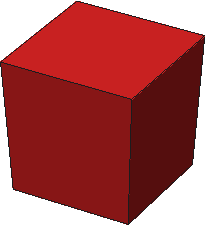
\includegraphics[width=\textwidth]{cubo}%
		\label{subfig:cubo}%
	\end{subfigure}%
	%
	\hspace{1.5cm}
	%
	\begin{subfigure}[b]{0.2\textwidth}
		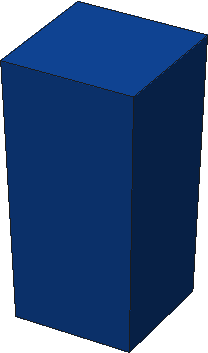
\includegraphics[width=\textwidth]{prisma}%
		\label{subfig:prisma}%
	\end{subfigure}%
	%
	\caption{Ejemplos de los objetos considerados para las clases $C_1$ (izquierda) y $C_2$ (derecha).}%
	\label{fig:objetos}%
\end{figure}
%
De los atributos posibles de estos objetos, el utilizado para diferenciar las clases de objetos es su altura $h$, el cual es suficiente para abordar el problema.

Así:
%
\begin{align}
	\label{eq:atributos_diferenciadores}
	A_k &= \{h_k\} \\
	\intertext{son los conjuntos de atributos asociados a cada objeto $o_k$, donde $h_k$ solo puede tener dos posibles valores, por lo cual las clases quedan definidas de la siguiente forma:}
	\begin{split}
		C_1 &= \{h_1\} \\[1em]
		C_2 &= \{h_2\} \rlap{${}= \{2h_1\}$}
	\end{split}
\end{align}
%
Para evaluar la propuesta en las diferentes configuraciones propuestas del espacio $E$, se utilizaron diferentes cantidades de objetos, siendo $N$ la cantidad total de objetos en dichos espacios, la cual será la suma de los objetos de ambas clases propuestas, donde $N_1$ es la cantidad de objetos de la clase $C_1$ y $N_2$ los objetos de la clase $C_2$.

En los casos tratados solo se permite colocar un objeto por cada celda de la malla y la cantidad $N$ debe cumplir la desigualdad $\left\lceil \frac{nm}{2} \right\rceil < N \leq nm$.
Esto porque una cantidad de objetos igual o menor a $\left\lceil \frac{nm}{2} \right\rceil$ se considera un caso con solución trivial; ya que siempre se dispone de espacio suficiente para acomodarlos en una configuración en la cual se puedan tomar con una sola acción.
Además, el número de objetos disponibles no debe exceder el número total de celdas.
 
Dicho lo anterior, los casos de interés para validar la propuesta de este trabajo, consisten en todas las configuraciones de objetos $N_1$ y $N_2$ que no correspondan a casos triviales ni imposibles (los cuales serán detallados en la Sección \ref{sec:casos_triviales_e_imposibles}).
Es por ello que se obtuvieron las condiciones para que un caso no sea trivial ni imposible, resultando las siguientes:
%
\begin{equation}
\label{eq:cond_casos_de_interes}
\begin{gathered}
	\left\lceil \frac{nm}{2} \right\rceil < N \leq nm \\[7pt]
	N = N_1 + N_2 \\[7pt]
	0 \leq N_1 \leq N - \left\lfloor \frac{n}{2} \right\rfloor \! \left\lfloor \frac{m}{2} \right\rfloor \\[7pt]
	0 \leq N_2 \leq N - \left\lfloor \frac{n}{2} \right\rfloor \! \left\lfloor \frac{m}{2} \right\rfloor
\end{gathered}
\end{equation}
%
Un análisis más profundo de estas condiciones se dará en la Sección \ref{sec:casos_triviales_e_imposibles}.
%
%
\subsection{Características de la vecindad}
\label{subsec:vecindad}
%
%
Para definir el estado de la vecindad $V_{ij}$ de una celda $e_{ij}$, se considerarán como celdas vecinas de una celda particular $e_{ij}$, aquellas celdas que se encuentran inmediatamente arriba (dirección positiva de $i$), abajo, a la derecha (dirección positiva de $j$) y a la izquierda de esta, como se ilustra en la Figura \ref{fig:vecindad}.
%
\begin{figure}[H]
	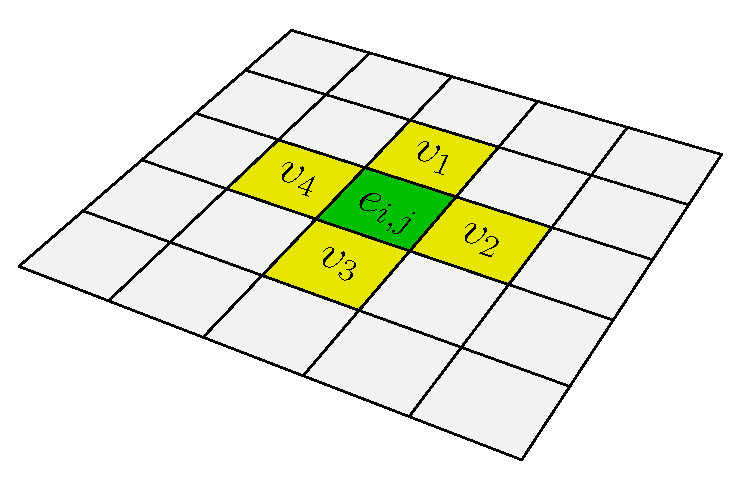
\includegraphics[width=0.6\textwidth]{vecindad}%
	\caption{Vecindad utilizada para abordar el problema planteado.}%
	\label{fig:vecindad}%
\end{figure}
%
El orden en el que se encuentran los estados de las celdas vecinas en el conjunto $V_{ij}$ se obtiene recorriendo las posiciones mencionadas en sentido horario comenzando con la celda de arriba, es decir:
%
\begin{equation}
	\label{eq:vecindad_usada}
	V_{ij} = \{v_1, v_2, v_3, v_4\}
\end{equation}
%
donde:
%
\begin{descriptionParams}
	\item[$v_1$] corresponde al estado de la celda $e_{i+1,\, j}$.
	\item[$v_2$] corresponde al estado de la celda $e_{i,\, j+1}$.
	\item[$v_3$] corresponde al estado de la celda $e_{i-1,\, j}$.
	\item[$v_4$] corresponde al estado de la celda $e_{i,\, j-1}$.
\end{descriptionParams}
%
Las características de la vecindad de los elementos en los bordes y esquinas de la malla no difiere de las de los demás elementos.
Esto debido a que en todos los arreglos tratados se considera un ``espacio extendido'' de trabajo, el cual consiste en suponer que el espacio $E$ se encuentra rodeado por celdas vacías, tal y como se muestra en la Figura \ref{fig:malla_extendida}.
En estas celdas hipotéticas no se puede colocar ningún objeto, ya que únicamente cumplen con la función de actuar como vecinas de los elementos en los bordes y esquinas de la malla, de manera que las mismas reglas de vecindad de los elementos centrales también puedan ser aplicadas en ellos.
%
\begin{figure}[H]
	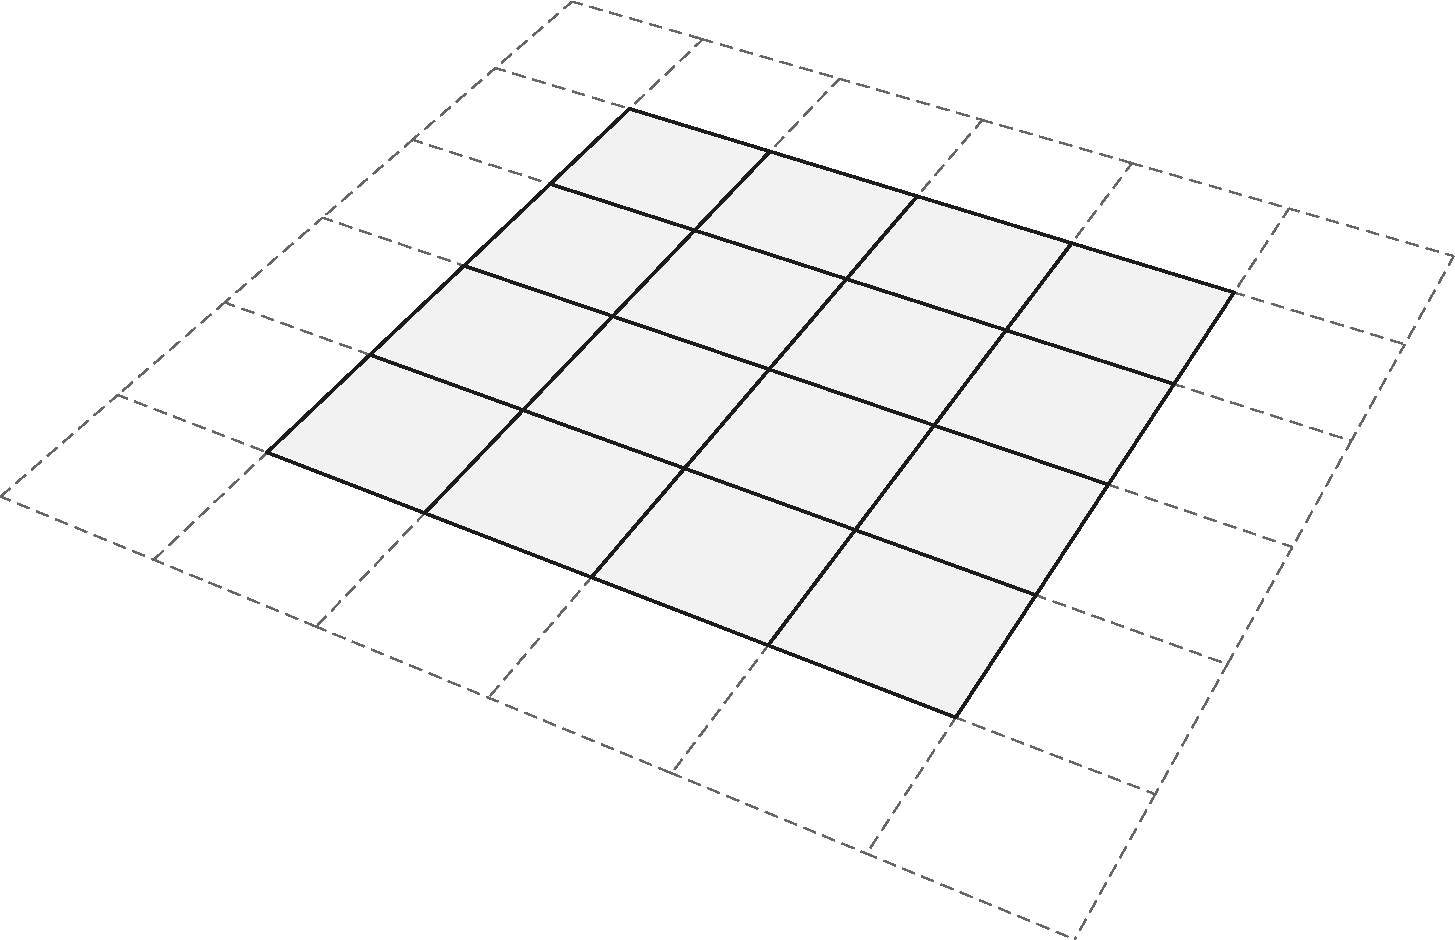
\includegraphics[width=0.6\textwidth]{malla_extendida_3D}%
	\caption{Ejemplo de espacio extendido en una malla de $4\times 4$.}%
	\label{fig:malla_extendida}%
\end{figure}
%
En todos los casos del presente trabajo se supondrá un espacio extendido como el de la Figura \ref{fig:malla_extendida}, pero esta característica puede ser modificada según las necesidades del problema que se aborde.
Por ejemplo, si se desea realizar el acomodo de objetos dentro de una caja, puede ser más adecuado cambiar las celdas vacías del espacio extendido por elementos fijos de determinada altura, a manera de pared.
%
%
\subsection{Formas de sujeción}
\label{subsec:formas_sujecion}
%
%
Solo se consideran dos formas de agarre, las cuales son comunes a ambas clases de objetos: agarre horizontal $H$ y agarre vertical $V$; esto es:
%
\begin{equation}
\label{eq:formas_sujecion_usadas}
	S = S_1 = S_2 = \{H, V\}
\end{equation}
%
Estas formas de agarre se establecieron considerando un manipulador que solo puede tomar los objetos por la parte superior.
Un esquema de los puntos que son utilizados, en teoría, para sujetar los objetos se muestra en la Figura \ref{fig:formas_sujecion}.
%
\begin{figure}[H]
	\begin{subfigure}{0.4\textwidth}
		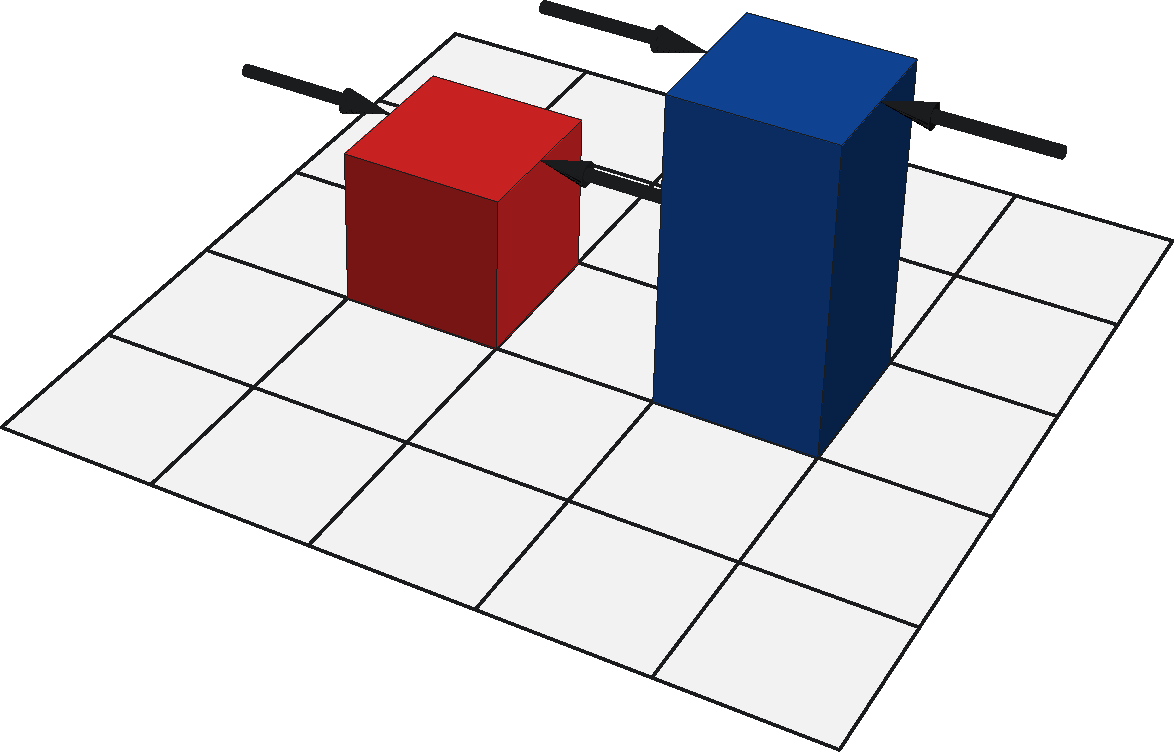
\includegraphics[width=\textwidth]{agarre_horizontal}%
		\label{subfig:sujecion_H}%
	\end{subfigure}%
	%
	\hspace{1cm}
	%
	\begin{subfigure}{0.4\textwidth}
		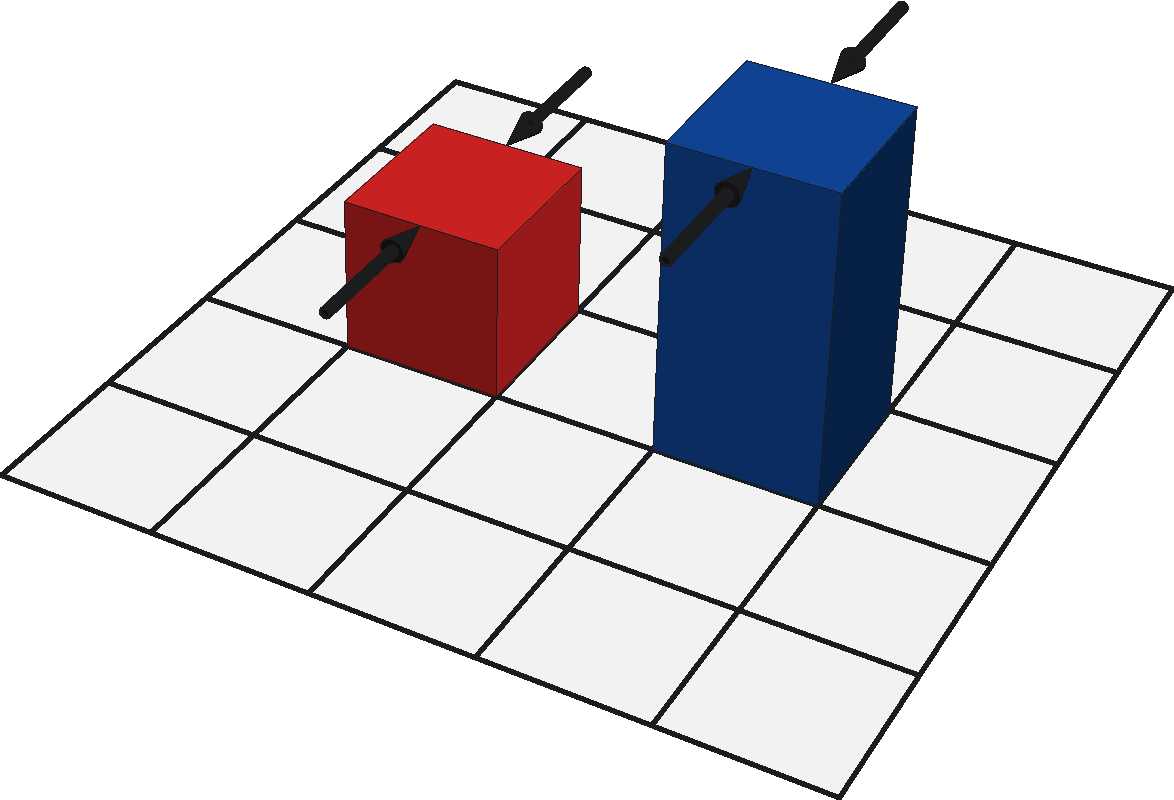
\includegraphics[width=\textwidth]{agarre_vertical}%
		\label{subfig:sujecion_V}%
	\end{subfigure}%
	\caption{Formas de sujeción horizontal (izquierda) y vertical (derecha).}%
	\label{fig:formas_sujecion}%
\end{figure}
%
%
\subsection{Restricciones de las formas de sujeción}
\label{subsec:restricciones}
%
%
Las formas de sujeción aplicables a cada clase de objeto pueden ser restringidas en función de su vecindad $V_{ij}$.

Un objeto $o_k$ puede ser sujetado de las formas $H$ y $V$ si sus vecinos horizontales y verticales, respectivamente, tienen una menor altura que el objeto $o_k$.
La definición matemática de la oración anterior se presenta en la Ecuación \ref{eq:restricciones} de la Sección \ref{sec:funciones_y_procedimientos}.

Algunos ejemplos de cómo se restringen las formas de sujeción de un objeto, en función de su vecindad, se muestran en la Figura \ref{fig:restricciones_agarre}.
%
\begin{figure}[H]
	\def\hsep{12pt}%
	\captionsetup[subfigure]{width=\textwidth}%
	\begin{subfigure}{0.31\textwidth}
		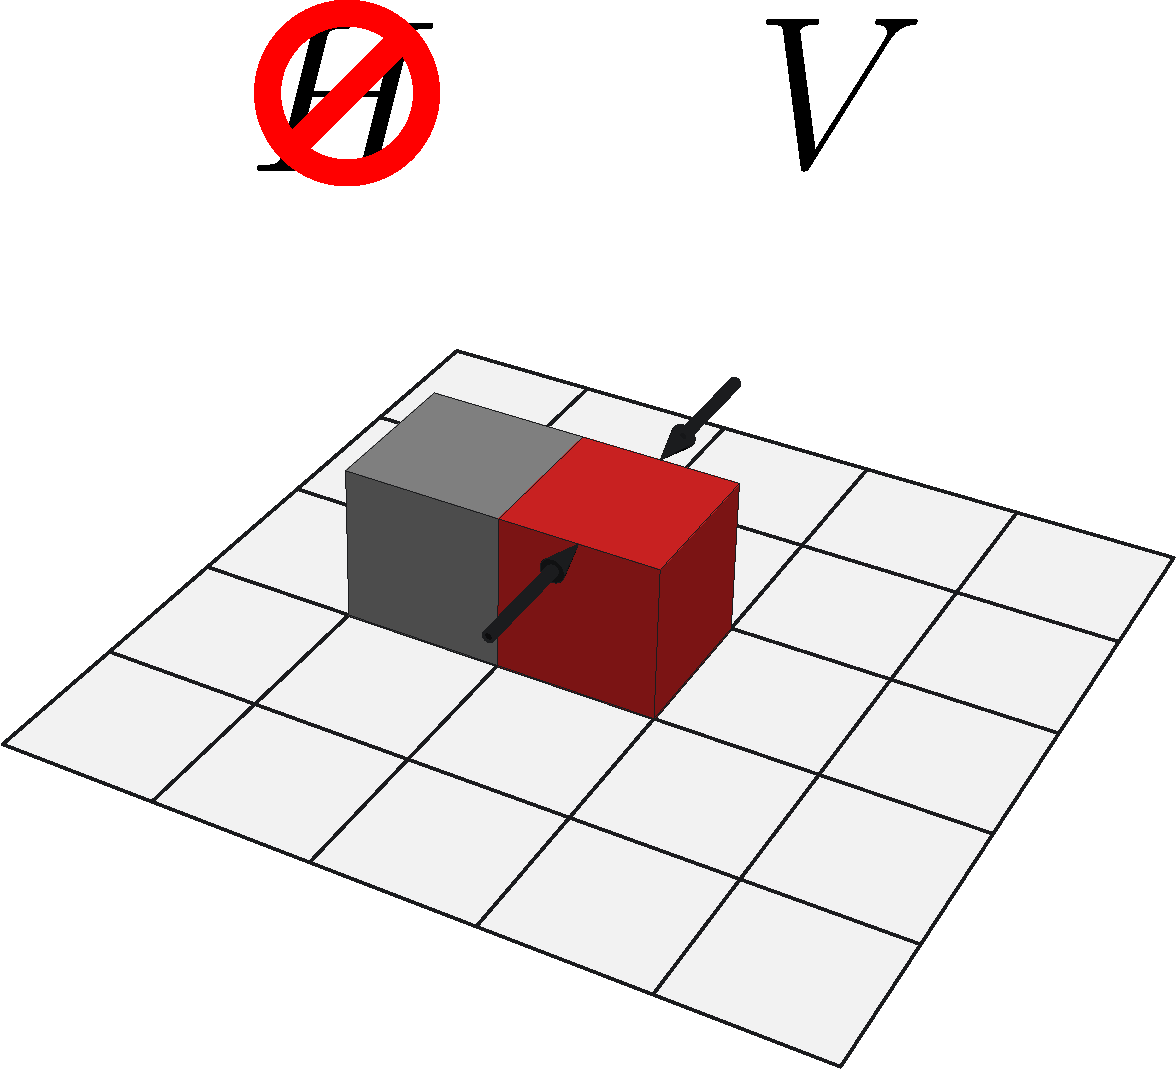
\includegraphics[width=\textwidth]{restriccion_H_cubo}%
		\label{subfig:restriccion_H_cubo}%
	\end{subfigure}%
	\hspace{\hsep}%
	\begin{subfigure}{0.31\textwidth}
		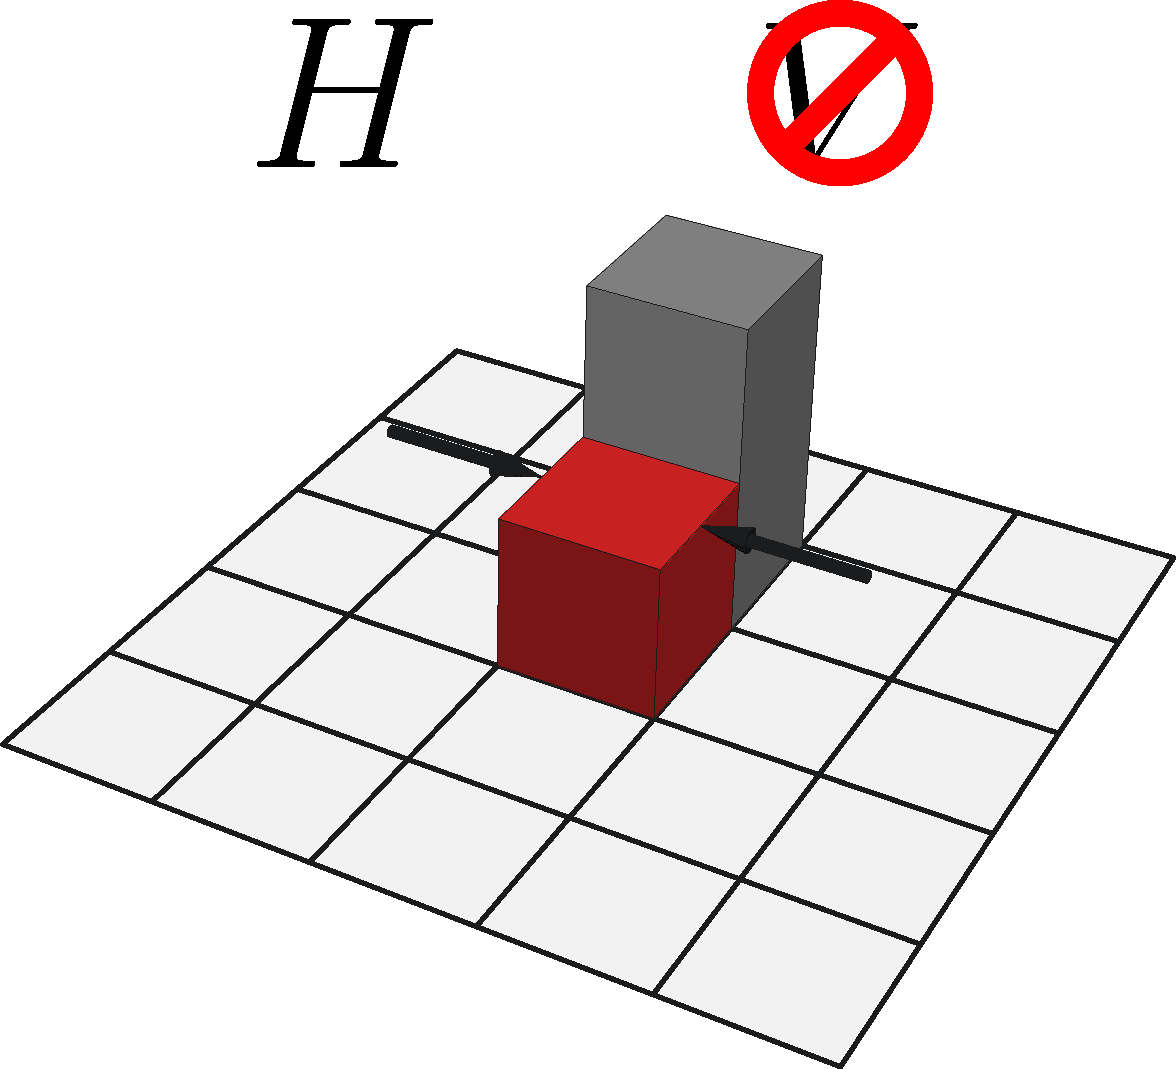
\includegraphics[width=\textwidth]{restriccion_V_cubo}%
		\label{subfig:restriccion_V_cubo}%
	\end{subfigure}%
	\hspace{\hsep}%
	\begin{subfigure}{0.31\textwidth}
		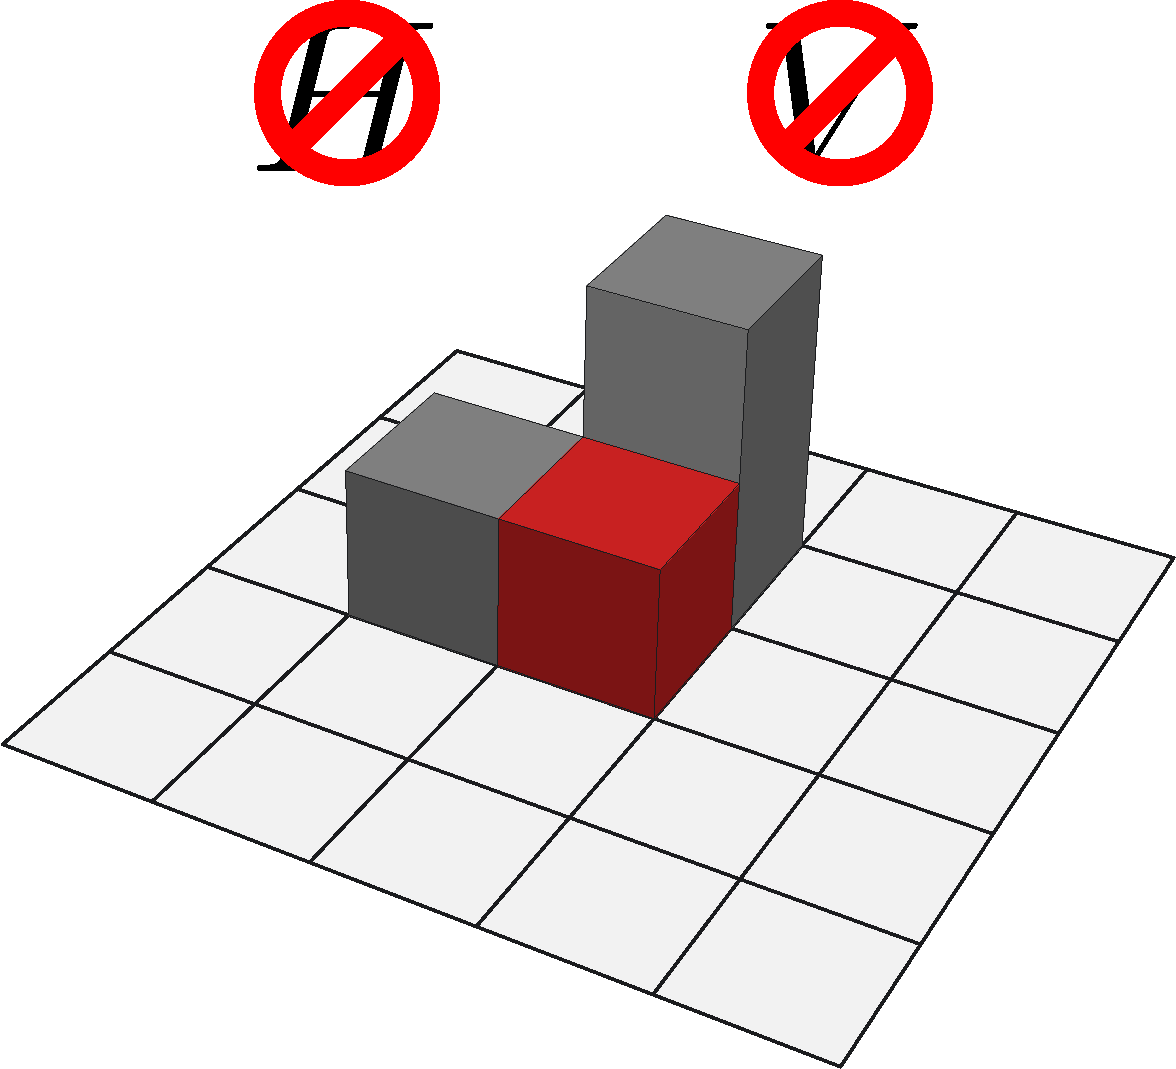
\includegraphics[width=\textwidth]{restriccion_HV_cubo}%
		\label{subfig:restriccion_HV_cubo}%
	\end{subfigure}%
	
	\vspace{0.7cm}
	%
	\begin{subfigure}{0.31\textwidth} 
		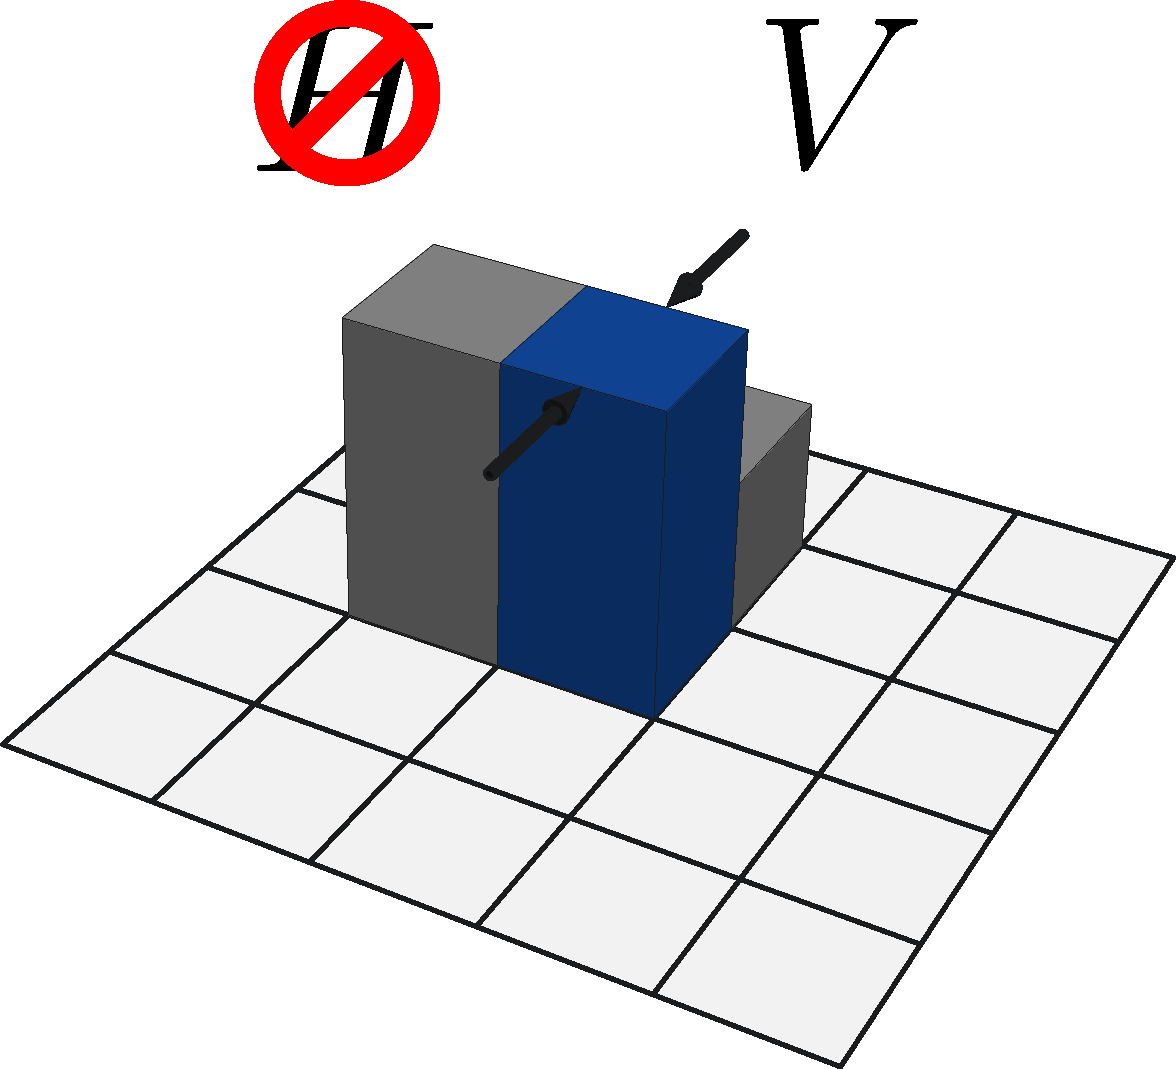
\includegraphics[width=\textwidth]{restriccion_H_prisma}%
		\label{subfig:restriccion_H_prisma}
	\end{subfigure}%
	\hspace{\hsep}%
	\begin{subfigure}{0.31\textwidth}
		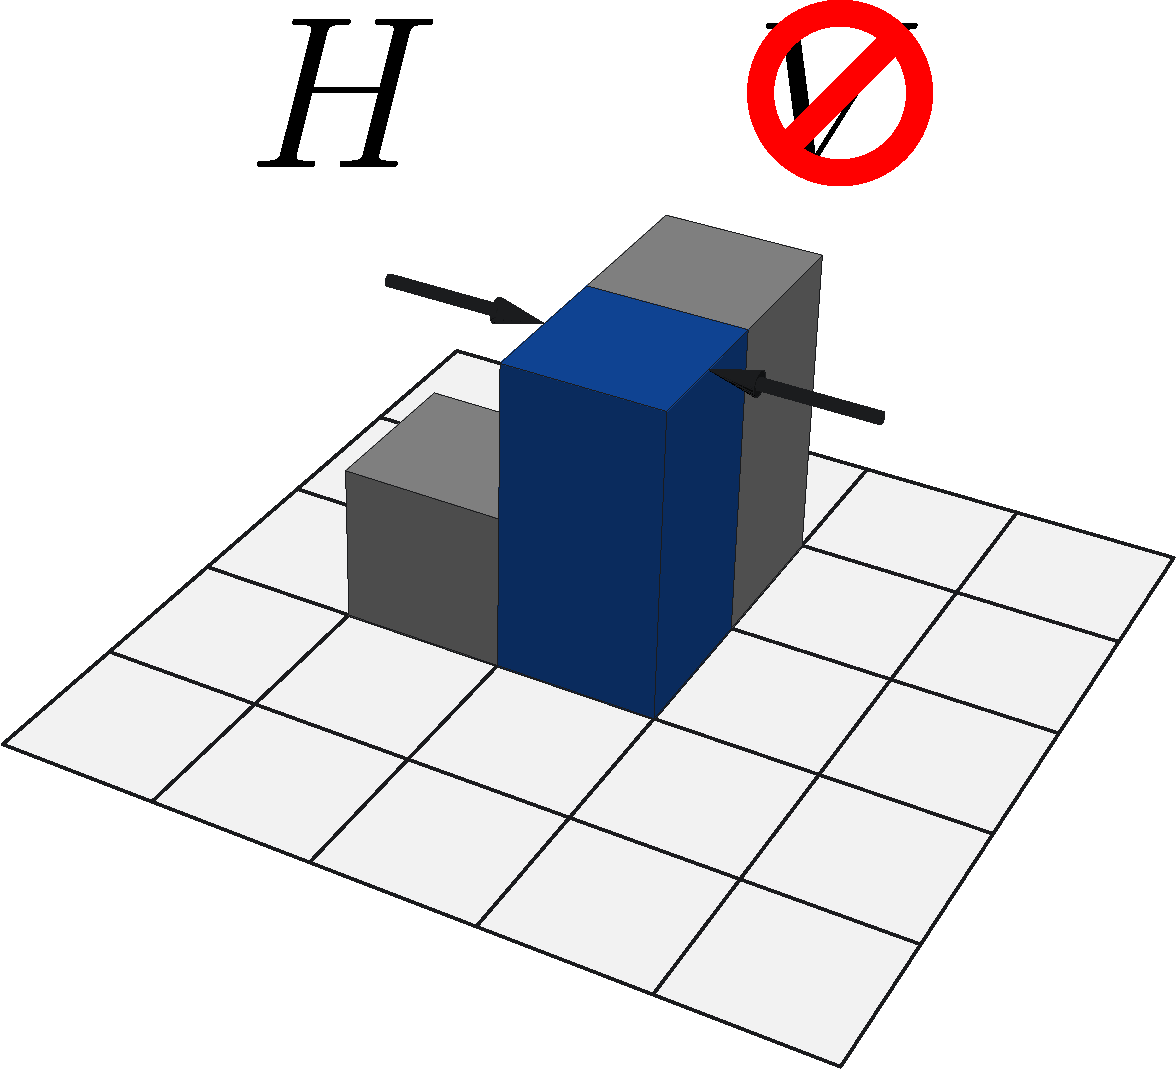
\includegraphics[width=\textwidth]{restriccion_V_prisma}%
		\label{subfig:restriccion_V_prisma}
	\end{subfigure}%
	\hspace{\hsep}%
	\begin{subfigure}{0.31\textwidth}
		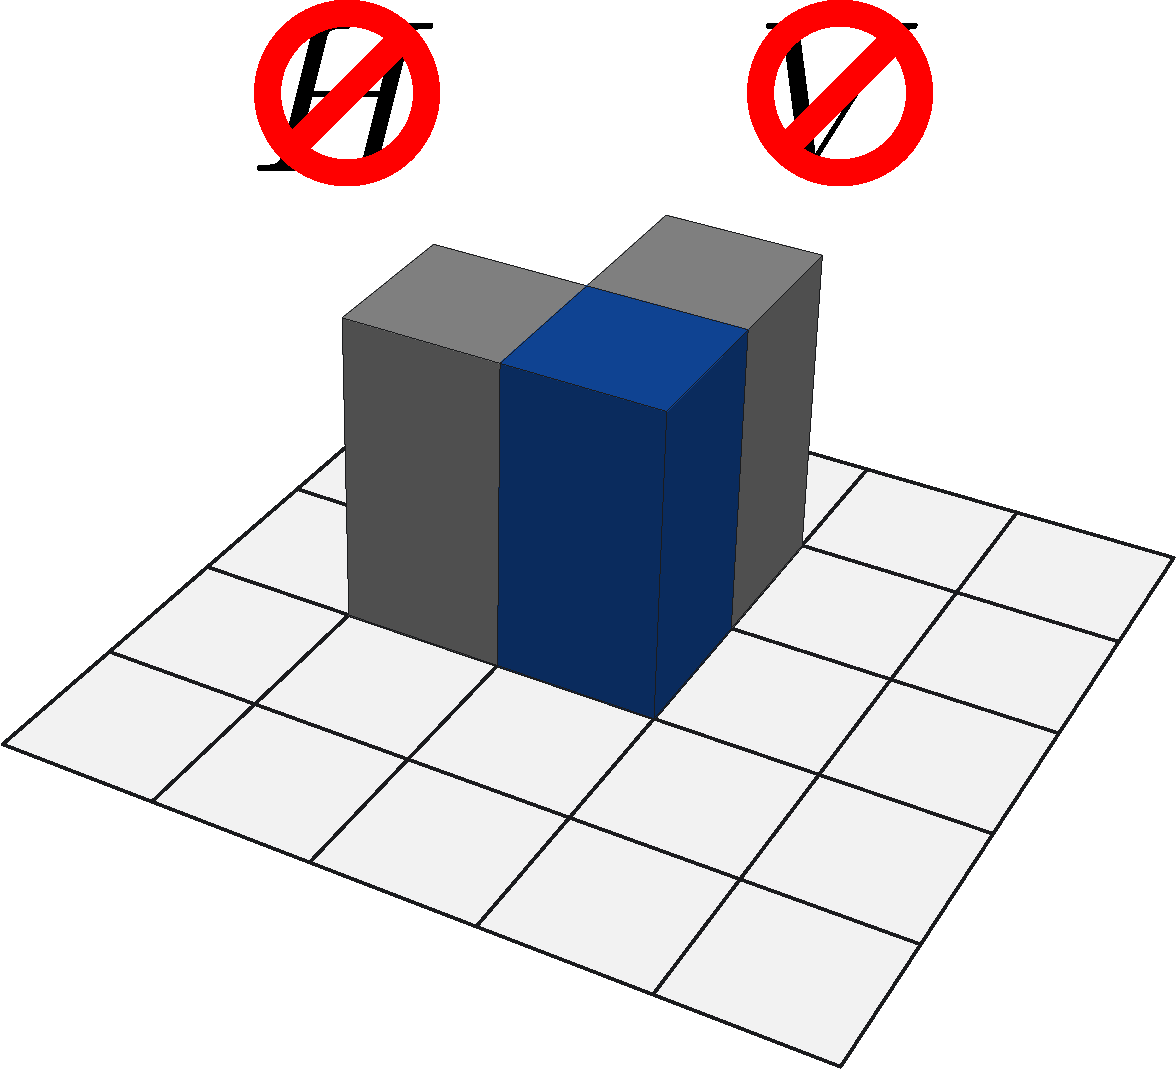
\includegraphics[width=\textwidth]{restriccion_HV_prisma}%
		\label{subfig:restriccion_HV_prisma}%
	\end{subfigure}%
	%
	\caption{Ejemplos de cómo se pueden restringir las formas de sujeción en función de la vecindad.}%
	\label{fig:restricciones_agarre}%
\end{figure}
%
%
\subsection{Acciones}
\label{subsec:acciones}
%
%
Por el momento solo se consideran dos tipos de acciones: poner un objeto en $E$ ($w_1$) y quitarlo de $E$ ($w_2$), es decir:
%
\begin{equation}
	\label{eq:acciones_usadas}
	W = \{w_1, w_2\}
\end{equation}
%
Se considera que estas acciones son suficientes para la primera aproximación propuesta para el problema planteado.
%
%
\subsection{Especificaciones adicionales}
\label{subsec:especificaciones_adicionales}
%
%
Los objetos no se pueden colocar uno encima de otro, por lo cual solo se pueden generar acomodos como el que se muestra en la Figura \ref{fig:muestra_acomodo}.

A diferencia del problema del contenedor, no se toma en cuenta el caso en que haya que dejar objetos sin acomodar por falta de espacio.
Ya que, si bien este sería un caso de estudio interesante, en el que se podrían fusionar las técnicas del problema del contenedor con las propuestas, se cree que el añadir este tipo de restricciones disfrazaría la esencia del verdadero problema que se quiere resolver.
Por lo cual se da por hecho que los $N$ objetos se pueden colocar sin problemas en $E$, es decir, ningún objeto debe quedar fuera de $E$ en el arreglo final.
%
\begin{figure}[H]
	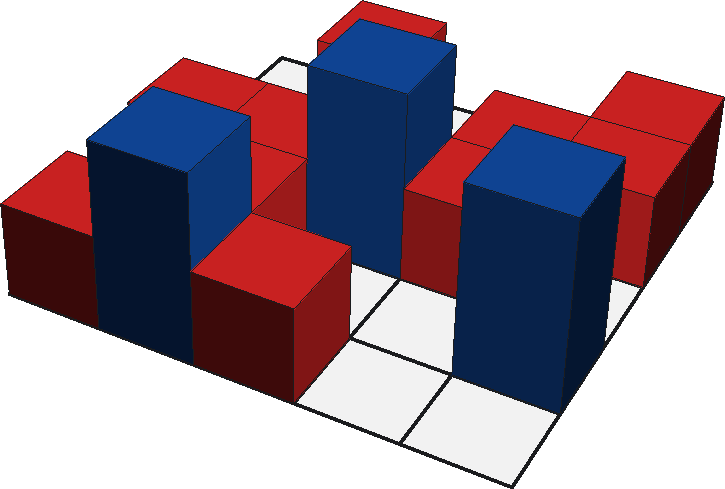
\includegraphics[width=0.63\textwidth]{arreglo_muestra}%
	\caption{Ejemplo de una configuración de objetos en la malla.}%
	\label{fig:muestra_acomodo}%
\end{figure}
%
%
\section{Análisis de complejidad del problema}
\label{sec:analisis_complejidad}
%
%
Debido a que el objetivo final del presente trabajo es encontrar una configuración específica de los objetos de $O$ en $E$, la complejidad del problema estará entonces relacionada con el total de configuraciones de objetos que se pueden generar a partir de dados: un conjunto $O$ de objetos y un espacio $E$ en el cual colocarlos.

Si se considera el espacio de búsqueda sobre todas las configuraciones posibles de objetos en la malla, utilizando el conjunto $O$ para la representación de los objetos y el símbolo $\boxslash$ para la representación de una celda vacía, se tiene el siguiente espacio de búsqueda:
%
\begin{equation}
	\label{eq:complejidad_1}
	\mathcal{C} = (O \cup \{ \boxslash \})^{nm}
\end{equation}
%
donde se ha hecho explícita la unión con la representación de una celda vacía, al considerarla como un elemento más del conjunto, debido a su recurrente uso.

Al utilizar el conjunto $O$ para la representación de los objetos, implícitamente se está considerando a cada uno de sus elementos como diferente a los demás, ya que, en general, sus respectivos atributos $A_k$ pueden ser diferentes.
Por lo cual el número de configuraciones posibles en dicho espacio viene dado por: 
%
\begin{equation}
	\label{eq:complejidad_2}
	|\mathcal{C}| = |O \cup \{ \boxslash \}|^{nm} = (N+1)^{nm}
\end{equation} 
%
Con la finalidad de reducir este espacio de búsqueda es que se ha establecido el sistema de clases definido anteriormente.
Mediante esta herramienta es posible identificar atributos clave $A_k$ de objetos no necesariamente iguales, los cuales permitan tratarlos como tal únicamente en lo que respecta a su sujeción.
Por ejemplo, si al tener una esfera y un cubo en el espacio $E$ se tiene la condición de que el manipulador solo es capaz de tomar estos objetos mediante una única posición y orientación, utilizando puntos de contacto semejantes; entonces, no tendría caso considerar estos objetos como diferentes, en lo que a su manipulación se refiere.
Por lo cual, para cuestiones de sujeción, lo conveniente sería representarlos como objetos de la misma clase.

Al hacer esta consideración el espacio de búsqueda puede ser reducido, ya que:
%
\begin{equation}
	\label{eq:complejidad_3}
	|C| \leq |O|
\end{equation}
%
por lo cual el nuevo espacio de búsqueda sería:
%
\begin{equation}
	\label{eq:complejidad_4}
	\mathcal{C}' = (C \cup \{ \boxslash \})^{nm}
\end{equation}
%
Y de forma similar a la Ecuación \ref{eq:complejidad_2}, el número de configuraciones posibles quedaría como:
%
\begin{equation}
	\label{eq:complejidad_5}
	|\mathcal{C}'| = |C \cup \{ \boxslash \}|^{nm} = (N_C+1)^{nm}
\end{equation}
%
Sin embargo, el espacio de búsqueda de interés para el problema enunciado, es un subconjunto de $\mathcal{C}'$, para el cual se tiene un número de objetos $N$ fijo, e igualmente las cantidades de objetos de cada clase $N_1, N_2, \ldots, N_{N_C}$ son también fijas.

Entonces, se define $\mathcal{C}''$ como el espacio de todas las configuraciones posibles de $N$ objetos de $N_C$ clases en un $E$ específico, donde $N_1, N_2, \ldots, N_{N_C}$ son cantidades fijas.
Para lo cual se define a $\mathcal{C}''_{\text{ins}}$ como cualquier instancia de $\mathcal{C}''$ y a $\mathcal{C}''_{\text{ins}}(C_K)$ como el número de veces que aparece la clase $C_K$ en $\mathcal{C}''_{\text{ins}}$.
Por lo tanto 
%
\begin{equation}
	\label{eq:complejidad_6}
	\mathcal{C}'' = (C \cup \{ \boxslash \})^{nm} \ | \ \mathcal{C}''_{\text{ins}}(C_K) = N_K,\ 1 \leq K \leq N_C
\end{equation}
%
lo cual establece que debe haber exactamente $N_1$ objetos de la clase $C_1$, $N_2$ de la clase $C_2$, etc., en cualquier instancia de $\mathcal{C}''$.

El número de configuraciones posibles para $\mathcal{C}''$ es entonces:
%
\begin{equation}
	\label{eq:complejidad_7}
	|\mathcal{C}''| = \frac{nm!}{N_1!N_2! \cdots N_{N_C}!(nm - N)!}
\end{equation}
%
En la Tabla \ref{tab:permutaciones_posibles} se muestra el número de configuraciones posibles para algunas combinaciones de valores del tamaño de la malla y del número de objetos de cada clase.
%
\begin{table}[H]
	\renewcommand{\arraystretch}{1.4}%
	\savetablewidth{%
	\begin{tabular}{ccccc}
		\hline
		\textbf{Tamaño malla} & $\bm{N_1}$ & $\bm{N_2}$ & $\bm{nm - N}$ & $\bm{|\mathcal{C}''|}$ \\ \hline
		\arrayrulecolor{gray!60}%
		$3\times 3$ & $3$ & $3$ & $3$ & $\num{1680}$ \\ \hline
		$3\times 3$ & $1$ & $5$ & $3$ & $504$ \\ \hline
		$3\times 3$ & $4$ & $5$ & $0$ & $126$ \\ \hline
		$4\times 4$ & $5$ & $5$ & $6$ & $\num{2018016}$ \\ \hline
		$4\times 4$ & $1$ & $9$ & $6$ & $\num{80080}$ \\ \hline
		$4\times 4$ & $8$ & $8$ & $0$ & $\num{12870}$ \\ \hline
		$5\times 5$ & $8$ & $8$ & $9$ & $2.62\times10^{10}$ \\ \hline
		$5\times 5$ & $10$ & $10$ & $5$ & $0.98\times10^{10}$ \\ \hline
		$5\times 5$ & $12$ & $13$ & $0$ & $\num{5200300}$ \\ \hline
		$6\times 6$ & $12$ & $12$ & $12$ & $3.38\times10^{15}$ \\ \hline
		$6\times 6$ & $15$ & $15$ & $6$ & $0.30\times10^{15}$ \\ \hline
		$6\times 6$ & $18$ & $18$ & $0$ & $9.07\times10^{9}$ \\ 
		\arrayrulecolor{maintextcolor}%
		\hline
	\end{tabular}%
	}%
	\captionsetup{width=\tablewidth}%
	\caption{Número de permutaciones de arreglos posibles en función del número de elementos de cada clase presentes en la malla y del tamaño de la malla.}%
	\label{tab:permutaciones_posibles}%
\end{table}
%
Al analizar la Tabla \ref{tab:permutaciones_posibles} se puede observar que, entre más uniforme sea la distribución del número de objetos de cada clase y de celdas vacías ($nm - N$), el número de permutaciones posibles de una malla aumenta.
Es decir, que cuando las cantidades de objetos de cada clase y de celdas vacías son lo más parecidas entre sí, es cuando el número de permutaciones es máximo, y disminuye conforme se va perdiendo esta uniformidad.
%
%
\section{Casos triviales y casos imposibles}
\label{sec:casos_triviales_e_imposibles}
%
%
Existen cantidades especiales de objetos $N$, así como del número de objetos de cada clase $N_1, N_2, \ldots, N_{N_C}$, para las cuales se pueden tener casos de acomodo triviales o imposibles.
Las características de estos casos se definen a continuación.

Un caso trivial es un caso en el cual la cantidad $N$ de objetos es lo suficientemente pequeña como para acomodar los objetos en un patrón simple, el cual permite que todos los objetos puedan ser sujetados con una sola acción.
En este caso los objetos pueden ser siempre colocados mediante un mismo patrón, previamente establecido, siempre que se cumpla la siguiente condición:
%
\begin{equation}
	\label{eq:condicion_triviales}
	N \leq \left\lceil \frac{nm}{2} \right\rceil
\end{equation}
%
Un patrón de acomodo para casos triviales se presenta en la Figura \ref{fig:casos_triviales}, dónde $N = \left\lceil \frac{nm}{2} \right\rceil$.
En el presente trabajo no se abordan este tipo de casos.
%
\begin{figure}[H]
	\begin{subfigure}{0.3\textwidth}
		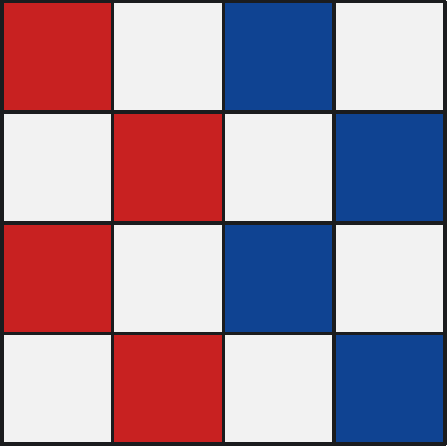
\includegraphics[width=\textwidth]{arreglo_trivial_4x4_2D}%
		\label{subfig:trivial_4x4}%
	\end{subfigure}%
	%
	\hspace{2.2cm}
	%
	\begin{subfigure}{0.3\textwidth}
		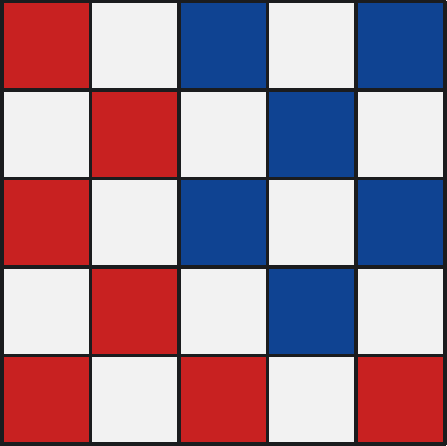
\includegraphics[width=\textwidth]{arreglo_trivial_5x5_2D}%
		\label{subfig:trivial_5x5}%
	\end{subfigure}%
	%
	\caption{Ejemplos de casos triviales en mallas de $4\times 4$ (izquierda) y $5\times 5$ (derecha).}
	\label{fig:casos_triviales}%
\end{figure}
%
Por otro lado, también existen configuraciones específicas de objetos en la malla, las cuales implican que algunos objetos sean imposibles de tomar, dadas las reglas de sujeción establecidas.
Estos casos se presentan cuando al menos cuatro objetos de la misma clase se agrupan en un patrón como el que se muestra en la subfigura izquierda de la Figura \ref{fig:casos_imposibles}.
En este caso ninguno de los cuatro objetos puede ser sujetado mediante las formas de sujeción definidas $H$ y $V$.
Estas agrupaciones de cuatro elementos de la misma clase se puede presentar una o varias veces en un acomodo de objetos, como se muestra en la subfigura derecha de la Figura \ref{fig:casos_imposibles}.

Se ha denominado como \textsl{cuadro imposible} al arreglo de cuatro objetos de la misma clase descrito anteriormente, y como \textsl{caso imposible} a un arreglo de objetos en la malla que contenga al menos un cuadro imposible.
%
\begin{figure}[H]
	\begin{subfigure}{0.3\textwidth}
		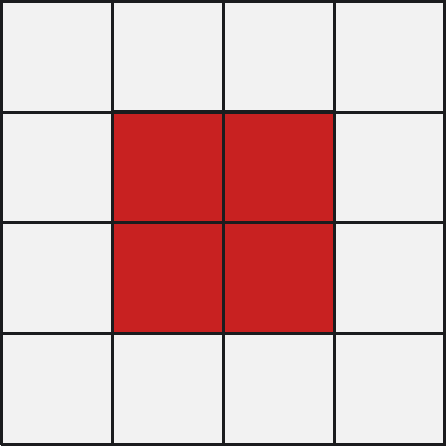
\includegraphics[width=\textwidth]{arreglo_imposible1_4x4_2D}%
		\label{subfig:imposibles_1}%
	\end{subfigure}%
	%
	\hspace{2.2cm}
	%
	\begin{subfigure}{0.3\textwidth}
		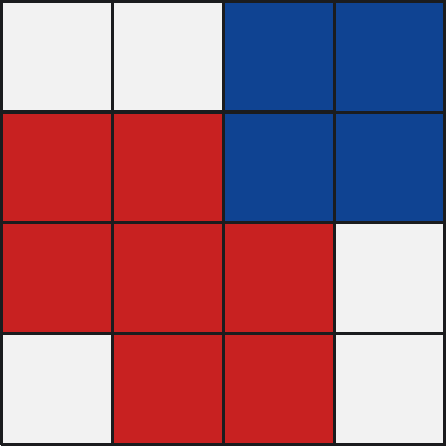
\includegraphics[width=\textwidth]{arreglo_imposible2_4x4_2D}%
		\label{subfig:imposibles_2}%
	\end{subfigure}%
	%
	\caption{Ejemplos de casos imposibles.}%
	\label{fig:casos_imposibles}%
\end{figure}
%
Los casos imposibles como los de la Figura \ref{fig:casos_imposibles} se pueden evitar con un acomodo correcto de los objetos en la malla.
Sin embargo existe una condición, la cual implica que siempre habrá cuadros imposibles en la malla, sin importar la forma en que se acomoden los objetos.

La condición para que exista al menos un cuadro imposible en un arreglo de objetos es:
%
\begin{equation}
	\label{eq:condicion_imposibles}
	\max_{K} N_K > nm - \left\lfloor \frac{n}{2} \right\rfloor \! \left\lfloor \frac{m}{2} \right\rfloor
\end{equation}
%
En el presente trabajo no se abordan este tipo de casos.

En el siguiente capítulo se presentarán los procedimientos y algoritmos desarrollados para abordar el problema propuesto.
Al final del capítulo se presentará el algoritmo principal que resuelve el problema planteado, el cual hace uso de los procedimientos que le preceden.
Posteriormente, en el Capítulo \ref{chap:resultados}, se presentarán los resultados obtenidos al aplicar el algoritmo principal a diferentes tamaños de malla y diferentes combinaciones de cantidades de objetos en ellas.
Finalmente, en el Capítulo \ref{chap:conclusiones}, se abordarán las conclusiones del proyecto.
% !TEX encoding = UTF-8 Unicode
\chapter{Desarrollo experimental}

%\markboth{Desarrollo experimental}{}

%Como se mencionó en la sección anterior, el sensor utilizado posee un sistema de medición \textcolor{red}{sigue sin quedar claro - ¿sistema de que?)} ortogonal de 3 ejes. 
%En el cual cada uno recopila datos de aceleración a lo largo de cada una de las direcciones en las que está dirigido, de manera que la información registrada sobre cada eje es independiente de la generada en los 2 restantes.\textcolor{red}{no se entiende la frase, sugiero recortar} 
%Se consideró que estas características son suficientes para obtener la información necesaria para el estudio de la dinámica de un vehículo.

Como se mencionó en la sección anterior, el sensor utilizado posee un sistema de medición ortogonal de tres ejes.
Cada uno recopila datos de aceleración a lo largo de la dirección en la que está dirigido. 
De manera que la información registrada sobre cada eje es independiente de la generada en los dos restantes.

Idealmente el sistema de ejes del sensor debe permanecer siempre fijo al vehículo, de tal manera que cualquier movimiento realizado por el vehículo sea igualmente realizado por el sensor. 
La configuración de ejes designada para el vehículo, a la cual se alineó el sensor de la forma más cercana posible, se describe a continuación: el eje $z$ es perpendicular al plano del suelo, el eje $x$ está dirigido a lo largo de la línea de movimiento principal del vehículo, siendo el eje $y$ perpendicular a los ejes $x$ y $z$. 
La configuración descrita se ilustra en la figura \ref{ejes}.

\begin{figure}[H]
\centering
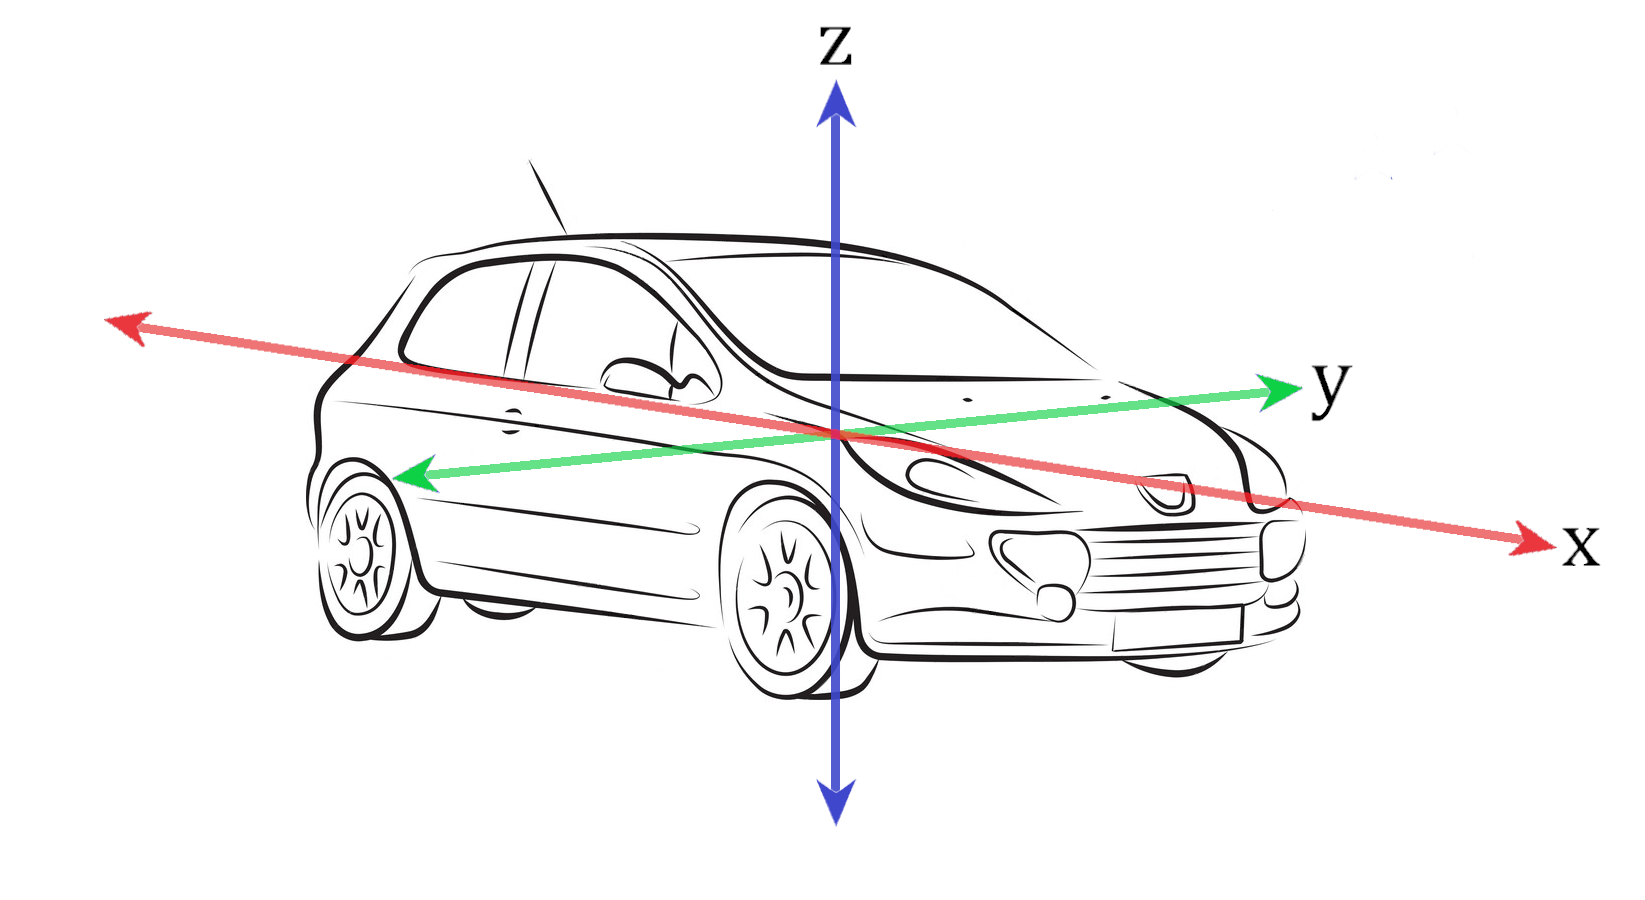
\includegraphics[scale=0.30]{car9.png}
\caption[Caption for LOF]{Sistema de ejes ortogonales\footnotemark[1].}
\label{ejes}
\end{figure}
\footnotetext[1]{Imagen modificada tomada de: https://www.vectorstock.com/royalty-free-vector/car-sketch-vector-98800}

Haciendo uso del equipo de medición, compuesto por el sensor de aceleración y el sistema GPS se realizaron diversas pruebas a bordo de un vehículo.

%\textcolor{orange}{(poner imagen del wiimote fijado al vehículo?)}\\

%El sensor fue colocado y alineado a la configuración de ejes antes mencionada\textcolor{red}{sigue igual (esto ya lo dijiste es redundante)}. 
%Una vez encendido, el sensor era identificado de manera inalámbrica por una computadora a bordo del vehículo, a la cual le transmitía los datos de aceleración de la misma manera, por medio de tecnología Bluetooth \textcolor{red}{si es por bluetooth ya es inalámbrico, sobra decirlo}. 

Una vez encendido, el sensor se comunicaba con una computadora a bordo del vehículo por medio de la tecnología Bluetooth, a la cual le transmitía los datos de aceleración.
Complementariamente se utilizó un dispositivo con GPS como apoyo para visualizar la trayectoria que se recorrería, con el fin de tener una mejor idea de cómo podría afectar la geometria de la ruta a las mediciones obtenidas por el sensor inercial a bordo del vehículo.

Para cada uno de los tres eventos (definidos en la primera sección) se designó una {\em etiqueta} con el propósito de diferenciarlos entre sí.
La etiqueta consistía en un carácter, diferente para cada evento, que el algoritmo registraba junto a los datos del evento correspondiente, cuando este tomaba lugar. 
Esta discriminación únicamente servía de ayuda al usuario para identificar más fácilmente los datos relativos a cada forma de conducir.

Adicionalmente se establecieron otras dos etiquetas para la obtención de datos, las cuales correspondían a una conducción regular y a una condición en la que el vehículo permanecía estático, pero con el motor encendido.
 
\section{Vehículo estático}

Lo primero en realizarse fue un registro de datos destinado únicamente para la etiqueta {\em vehículo estático}. 
Esto simplemente consistió en dejar el vehículo encendido y sin moverse en una superficie plana horizontal, por un lapso de $22s$.
Lo anterior se realizó con el objetivo de estudiar el espectro de frecuencias correspondiente a la señal obtenida por el sensor, buscando la posible presencia de algunas frecuencias con una amplitud significativa, esto es, superior a las demás. 
De ser así, dichas frecuencias corresponderían a las frecuencias fundamentales de vibración del motor, las cuales serían una fuente de ruido que perturbaría la exactitud de las mediciones de aceleración del vehículo. 
Durante el periodo de obtención de datos se verificó que el sensor se mantuviera fijo a la superficie a la que se adhirió, sin sufrir ningún tipo de deslizamiento, giro o desprendimiento de esta.

\section{Conducción regular}

El primer recorrido para el que se realizaron mediciones de aceleración fue el dedicado a la conducción regular. 
El cual consistió en conducir el vehículo de una manera conservadora, sin realizar ningún movimiento fuera de lo normal, a una velocidad de aproximadamente $80 km/h$ (dicha velocidad se considerará en adelante como el valor de {\em velocidad regular}).
Este recorrido tuvo una duración de aproximadamente $115 s$. %y consistió en conducir el vehículo en línea recta, en una superficie plana horizontal, a una velocidad regular, manteniéndolo lo más estable posible.

La conducción fue realizada sobre una superficie plana horizontal; y la ruta a seguir, tanto para este como para los posteriores recorridos, constaba de tramos rectos con algunas curvas suaves entre ellos, como se puede apreciar en la figura \ref{ruta} $b)$.\\
\pagebreak

\begin{figure}[H]
\begin{textblock*}{190mm}(5cm,7.5cm)
$a)$

\vspace{6.8cm}

$b)$
\end{textblock*}
\centering
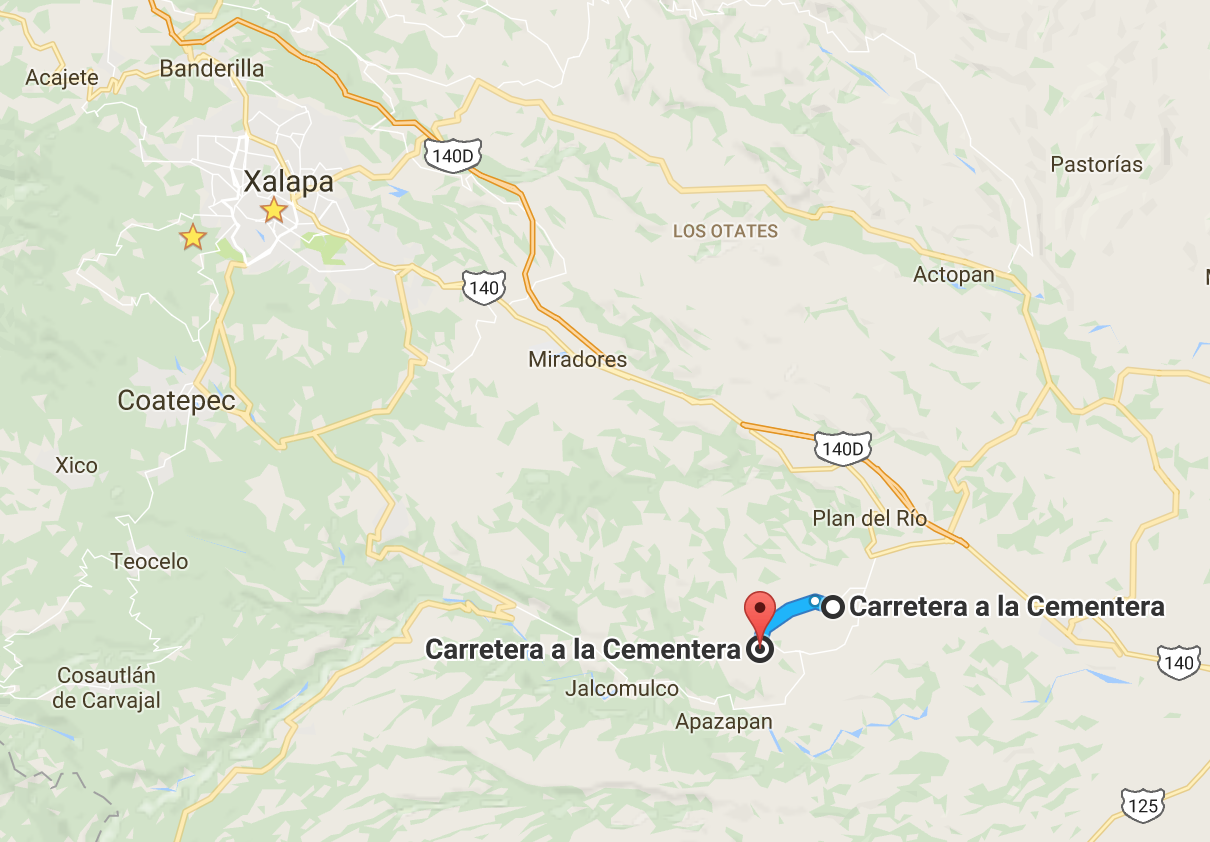
\includegraphics[scale=0.49]{Captura2.png}

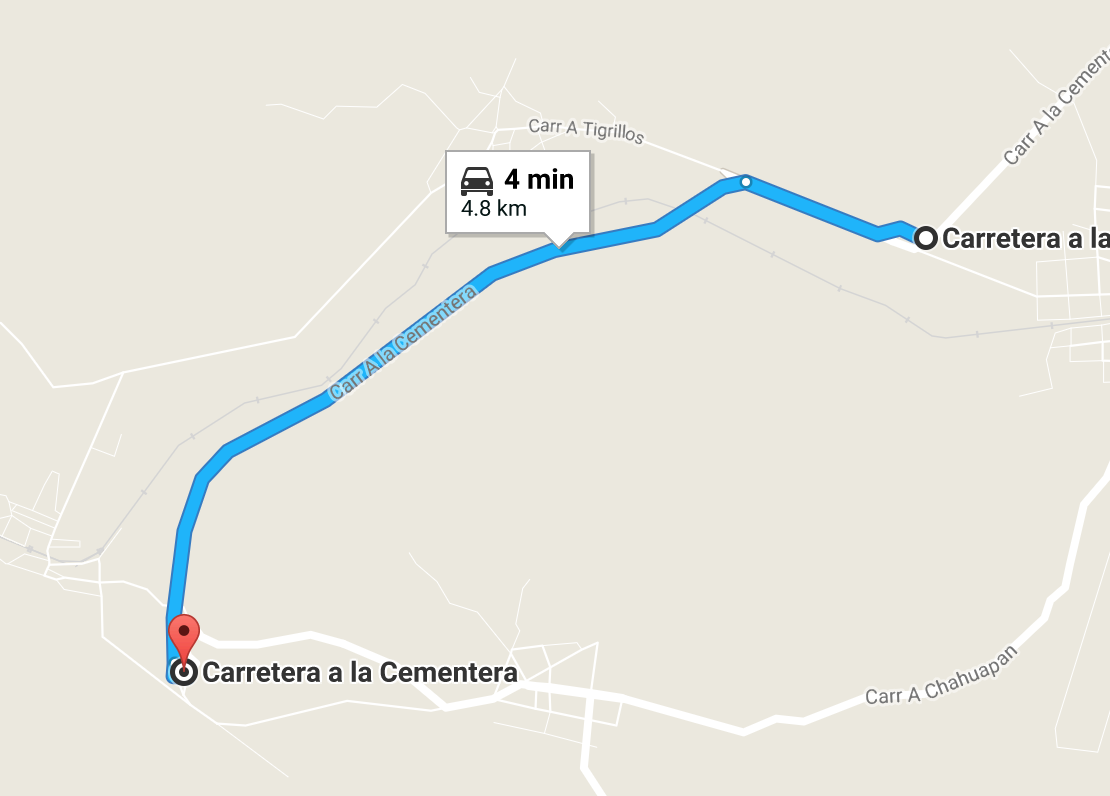
\includegraphics[scale=0.534]{Captura1.png}
\caption{$a)$ Ubicación de la ruta. $b)$ Ruta recorrida.}
\label{ruta}
\end{figure}

La recopilación de los datos para el modo de conducción regular se realizó con la finalidad de analizar el espectro de frecuencias de su señal y compararlo con el de los demás eventos. 
Esto para verificar que los espectros de frecuencias de los eventos detectables tuviesen características distintas a los de una conducción regular. 
Ya que, de no presentarse características suficientes para diferenciar los espectros de frecuencias de una conducción regular con respecto a los correspondientes a eventos, esto causaría problemas para discriminarlos entre sí analíticamente. 
Además, se verificó que no hubiese registros fuera de lo ordinario en la señal obtenida durante el recorrido; lo cual, de ser así, sería indicativo de alguna falla en los dispositivos utilizados.

Luego de obtener los datos correspondientes al vehículo estático y a una conducción regular, los cuales tendrían un papel complementario en el análisis, se inició con la recopilación de las señales asociadas a los eventos que se deseaban detectar.

\section{a) Evento de frenado}

El segundo recorrido realizado fue el dedicado al evento de frenado, el cual tuvo una duración total de $234s$ y consistió en varias conmutaciones entre conducciones regulares y eventos de frenado. 

Durante el trayecto se realizaron cuatro eventos de frenado, comenzando con una conducción regular. 
Se avanzó a la velocidad regular correspondiente, en la cual se evitó realizar cualquier movimiento anómalo que dificultara el posterior análisis.

Después haber transcurrido aproximadamente $84s$ de conducción regular se realizó el primer evento de frenado. 
Se frenó en un periodo de tiempo de aproximadamente $3s$, de manera que el vehículo quedó completamente detenido. 
Después de haber frenado al vehículo se comenzó a acelerar hasta recuperar la velocidad regular. 
Una vez que se había alcanzado la velocidad deseada se dio por culminado el evento de frenado, dando lugar a la conducción regular nuevamente. 
Desde que el vehículo comenzó a frenar hasta terminar el evento transcurrieron $15s$.

Los tres eventos de frenado restantes se realizaron de forma similar al primero. 
Los eventos que tuvieron mayor duración de los cuatro tardaron $18$ y $19s$ en llevarse a cabo, mientras que los dos restantes se ejecutaron en un periodo de $15s$ aproximadamente.

Todos los eventos de frenado que se realizaron durante este recorrido trataron de efectuarse de manera que fueran lo más parecidos posible entre sí, con la finalidad de que el patrón correspondiente a su dinámica quedara bien establecido, para que de esta forma su detección no presentara mayores dificultades. 
Todos los frenados se realizaron mientras el vehículo avanzaba en línea recta, los tramos curvos se asignaban a la conducción regular.

\section{b) Evento de rebase}

Después de haber recopilado los datos correspondientes al recorrido en el que se ejecutaron los eventos de frenado, se procedió a realizar otro recorrido, el cual estaría enfocado en capturar datos del evento rebase.

El recorrido dedicado al evento de rebase tuvo una duración total de $173s$, durante los cuales, al igual que con el evento de frenado, se cambió entre el modo de conducción regular y el evento de rebase en varias ocasiones. 

Se realizaron un total de tres eventos de rebase para este recorrido, comenzando con un tramo de conducción regular, seguido del primer evento de rebase. 
Para lo cual el piloto realizó la maniobra de un rebase común; aumentando la velocidad hasta un valor por encima de la velocidad regular, de aproximadamente $100km/h$, al mismo tiempo que desplazaba al vehículo hacia el carril adyacente de una manera moderada. 
Luego se avanzó durante algunos segundos sobre este carril, para posteriormente incorporarse de nuevo al carril de transito normal respectivo, de forma igualmente moderada. 
Después de lo cual se comenzó a reducir la velocidad hasta recuperar la que se tenía antes de ejecutar el rebase. 
Con esto se dio por finalizado el evento de rebase y se pasó al modo de conducción regular nuevamente. 
El primer evento de rebase para este recorrido duró un total de $19s$.

Los dos eventos de rebase siguientes se llevaron a cabo en forma semejante al primero, siendo de 20 y $16s$ los de mayor y menor duración.
Todos los rebases fueron hechos en tramos rectos y prácticamente horizontales, las trayectorias curvas se condujeron en modo de conducción regular.

\section{c) Evento de movimiento en zig-zag}

Luego de la recopilación de los datos correspondientes a los eventos de rebase y de frenado se llevó a cabo el recorrido dedicado al evento de movimiento en zig-zag. 
%Este recorrido tuvo una duración total de aproximadamente 265 segundos, durante los cuales se realizaron 4 eventos de zig-zag más un evento extra de rebase \textcolor[rgb]{1,0,0}{(esto es irrelevante)}. 
%El evento de rebase fue realizado con la finalidad de tener un número igual de muestras para cada tipo de evento, ya que tanto en el recorrido del evento de frenado como en el de zig-zag se realizarían 4 eventos en total. 
%Entonces, para efectuar un mejor análisis, se decidió aumentar el número de muestras añadiendo otro evento de tipo rebase.
Este recorrido tuvo una duración total de aproximadamente $265s$, durante los cuales se realizaron cuatro eventos de zig-zag y uno de rebase.

El recorrido consistió, al igual que los anteriores, en cambios entre conducción regular y los eventos que se querían detectar (zig-zag y rebase para este caso). 

Se inició el recorrido partiendo de una conducción regular, alcanzando una velocidad de $80km/h$.
El primer evento de movimiento en zig-zag se realizó después de este periodo; consistió en mover al vehículo de izquierda a derecha sobre el eje $y$ en repetidas ocasiones, usando el ancho de la pista. 
La frecuencia con la que se realizaban las oscilaciones era relativamente elevada, tratando de simular lo más parecido posible el caso real de un evento de tales características, en el que no se tiene el suficiente control del vehículo.

El evento de movimiento en zig-zag finalizó al dejar de realizar los movimientos de un lado a otro e incorporarse lentamente al carril correspondiente. 
Este evento tuvo una duración de $11s$, durante el cual se realizaron tres oscilaciones.

Los tres eventos de movimiento en zig-zag restantes fueron ejecutados de forma análoga al primero, con la diferencia de que tuvieron diferente número de oscilaciones: efectuando cuatro oscilaciones para el segundo, cinco para el tercero y seis para el cuarto; siendo este último el de mayor duración con $23s$.
Los tiempos de duración de los eventos fueron directamente proporcionales al número de oscilaciones.

El evento de rebase realizado en este recorrido tuvo una duración de aproximadamente $10s$. 
El cual se realizó imitando de la manera más parecida posible, las características de los rebases realizados en el recorrido dedicado a estos eventos.

Todos los eventos correspondientes a los movimientos en zig-zag, al igual el evento de rebase, se realizaron a lo largo de trayectos rectos, prácticamente horizontales y sin ninguna imperfección importante sobre el camino que pudiera representar un problema para el análisis o la adquisición de datos. 
Los tramos curvos se recorrieron en modo de conducción regular.

\section{Recorrido para validación}

Por último se realizó un recorrido adicional, en el cual se ejecutaron los tres eventos que se deseaban detectar: el frenado, el rebase y el movimiento en zig-zag. 
Esto con el fin de tener un conjunto de datos al cual posteriormente someter a una prueba de detección de los eventos de interés. 
Con el propósito de corroborar que los métodos empleados en la detección de tales eventos funcionasen de manera correcta, y de ser así, cumplir con el principal objetivo de este trabajo.

El recorrido consistió en ejecutar una vez cada uno de los tres eventos mencionados anteriormente. 
Antes y después de cada evento detectable se estableció la realización del tipo de pilotaje correspondiente a una conducción regular. 
Esto con la finalidad de que, al someter los datos a las pruebas de detección, el algoritmo pudiera diferenciar entre este tipo de conducción y los eventos que se esperaba fueran detectados.

En total, este recorrido tuvo una duración de $142s$.
Se inició el recorrido manejando el vehículo de una manera moderada, correspondiente a una conducción regular.

El primer evento en ejecutarse fue el movimiento en zig-zag, el cual consistió en mover el vehículo sobre el eje $y$, tal y como se describió en la sección dedicada a este evento.
El evento finalizó al dejar de realizar oscilaciones sobre el eje $y$, realizando un total de cinco oscilaciones. 
La duración de este evento fue de $17s$ y durante su ejecución se procuró que las características del evento fueran lo más parecidas posibles a los eventos de zig-zag realizados anteriormente.

El segundo evento detectable del recorrido fue el evento de frenado, el cual tuvo una duración de $17s$, durante los cuales se ejecutó la maniobra imitando las características de los eventos de frenado realizados anteriormente.

El último evento efectuado en este recorrido fue el evento de rebase, cuya ejecución tardó $14s$. 

%Los eventos realizados en este recorrido se llevaron a cabo sobre trayectos rectos y horizontales, los cuales no presentaban irregularidades que afectaran la conducción deseada o la correcta recopilación de datos. 
%Los trayectos curvos fueron recorridos durante los intervalos de tiempo en los que se efectuó la conducción regular.

Con la culminación de este recorrido se dio por terminada la recopilación de datos. 
Se decidió que se tenían las muestras suficientes para realizar un análisis adecuado en busca de los resultados deseados.
La información de cada recorrido se resume en la tabla \ref{tablarecorridos}.\\

\renewcommand{\arraystretch}{1.5}

\begin{table}[H]
\centering
\begin{tabular}{>{\centering\arraybackslash} m{4cm}|>{\centering\arraybackslash} m{2cm}|>{\centering\arraybackslash} m{2.5cm}|>{\centering\arraybackslash} m{2.7cm}}
%\toprule[1.2pt]
\hline \hline
\bf Nombre del recorrido o prueba & \bf Duración total & \bf Eventos realizados & \bf Duración de 
cada evento \\ 
\hline \hline 
%\Gape[1cm][1cm]
%\addlinespace
%\midrule
Vehículo estático & $22\ s$ & Ninguno & - \\ \hline
%\midrule
Conducción regular & $115\ s$ & Ninguno & - \\ \hline
%\midrule
\multirow{4}{*}{Frenado} & \multirow{4}{*}{$234\ s$} & $1^\text{er}$ Frenado & $15\ s$ \\ \cline{3-4}
& & $2^\text{o}$ Frenado & $19\ s$ \\ \cline{3-4}
& & $3^\text{er}$ Frenado & $15\ s$ \\ \cline{3-4}
& & $4^\text{o}$ Frenado & $18\ s$ \\ \hline
%\midrule
\multirow{3}{*}{Rebase} & \multirow{3}{*}{$173\ s$} & $1^\text{er}$ Rebase & $19\ s$ \\ \cline{3-4}
& & $2^\text{o}$ Rebase & $16\ s$ \\ \cline{3-4}
& & $3^\text{er}$ Rebase & $20\ s$ \\ \hline
%\midrule
\multirow{5}{*}{Movimiento en zig-zag} & \multirow{5}{*}{$265\ s$} & $1^\text{er}$ Zig-zag & $11\ s$ \\ \cline{3-4}
& & $1^\text{er}$ Rebase & $10\ s$ \\ \cline{3-4}
& & $2^\text{o}$ Zig-zag & $15\ s$ \\ \cline{3-4}
& & $3^\text{er}$ Zig-zag & $19\ s$ \\ \cline{3-4}
& & $4^\text{o}$ Zig-zag & $23\ s$ \\ \hline
%\midrule
\multirow{3}{*}{Recorrido para validación} & \multirow{3}{*}{$142\ s$} & $1^\text{er}$ Zig-zag & $17\ s$ \\ \cline{3-4}
& & $1^\text{er}$ Frenado & $17\ s$ \\ \cline{3-4}
& & $1^\text{er}$ Rebase & $14\ s$ \\
\hline \hline
%\bottomrule[1.2pt]
\end{tabular}
\caption{Información más relevante de cada recorrido.}
\label{tablarecorridos}
\end{table}

En este capítulo se describieron las condiciones en las que se llevaron a cabo las mediciones para esta investigación.
%\textcolor{blue}{Como comentario final de este capítulo se puede puntualizar que las condiciones en las que se llevaron a cabo las mediciones para esta investigación fueron las idóneas para su realización.
Todos los recorridos se realizaron sobre la misma ruta. 
No se presentaron problemas por parte del vehículo o del equipo de cómputo utilizado. 
Además de que la alineación y correcta obtención de datos por parte del equipo de medición (acelerómetro y GPS) fueron cuidadas a lo largo de los recorridos.
En el siguiente capítulo se describirá el análisis realizado con estos datos.

% !TEX encoding = UTF-8 Unicode
\chapter{Tratamiento de datos y resultados} 

Durante el desarrollo de este capítulo se analizarán los resultados obtenidos al aplicar las técnicas anteriormente mencionadas a los datos recopilados.

\section{Caracterización de los eventos}

En primer lugar se decidió construir las gráficas correspondientes a las señales adquiridas por el acelerómetro durante los recorridos.
Se resaltan en diferentes colores las señales correspondientes a cada evento detectable: rojo para el evento de frenado, verde para el evento de rebase y magenta para el evento de movimiento en zig-zag. 
Los datos relativos al modo de conducción normal se encuentran en color azul. 

A continuación se presentan las gráficas correspondientes a la aceleración registrada con respecto al tiempo transcurrido en los recorridos. 
Cada gráfica contiene información de uno de los tres ejes sobre los que se encontraba alineado el sensor.

Las unidades de aceleración en el eje $y$ de las gráficas corresponden a un formato específico que maneja el sensor utilizado; si se desean conocer las cantidades correspondientes en $m/s^2$ basta con aplicar la siguiente conversión; donde $x$ es la aceleración manejada por el sensor y $a$ es el valor de la misma en $m/s^2$.\\

$$a={9.81\over 25.5}(x-127)$$

\ \\

esta ecuación fue determinada al calibrar el sensor.\\

La gráfica de la señal obtenida en la prueba del vehículo estático muestra un comportamiento oscilatorio, de amplitud relativamente pequeña en comparación con los cambios de aceleración manejados en los recorridos, cuyos valores máximos son cercanos a $g$ (el valor correspondiente a $g$ en el formato del sensor es aproximadamente 25.5 unidades).
Únicamente se presenta la señal obtenida sobre el eje $z$ (figura \ref{1z2.pdf}) debido a que es el eje sobre el cual se registra la aceleración debida a la vibración del motor, además de que las señales de los ejes restantes tienen una forma similar\zsavepos{similar}.
\vspace{12.2cm}
\graficaceroeventos{1z2.pdf}{Vehículo estático}{z}{\dimexpr\paperheight-\zposy{similar}sp+10mm}

Al analizar los resultados de esta prueba se concluyó que la contribución al ruido en la señal por parte del motor y otros factores externos era irrelevante; ya que, tanto en la prueba del vehículo estático como en una situación en donde el acelerómetro permanece inmóvil en una superficie plana, se obtienen señales cuya amplitud, en promedio, no varía significativamente de una prueba a otra.
Por lo cual la oscilación de esta señal es principalmente debida al ruido blanco inherente al sensor; y debido a ello, el ruido provocado por los factores mencionados se considera como despreciable.
De no ser así, la vibración del motor provocaría que la amplitud promedio de la señal obtenida fuese mayor que la obtenida al dejar el sensor sobre una superficie inmóvil.

Los registros de aceleración de la prueba de conducción regular (figuras \ref{2x.pdf}, \ref{2y.pdf} y \ref{2z.pdf}) no presentan, como se esperaba, ninguna anomalía importante, exceptuando la cresta presente en los datos registrados en el eje $y$ del sensor, la cual es debida a la aceleración centrípeta generada al recorrer una curva.
\pagebreak

\ \\
\vspace{27cm}
\graficaceroeventos{2x.pdf}{Conducción regular}{x}{40mm}
\graficaceroeventos{2y.pdf}{Conducción regular}{y}{147mm}
\pagebreak
\ \\
\vspace{10.4cm}
\graficaceroeventos{2z.pdf}{Conducción regular}{z}{40mm}

Durante el recorrido destinado para el evento de frenado se obtuvieron los siguientes registros (figuras \ref{3x.pdf}, \ref{3y.pdf} y \ref{3z.pdf}):
\pagebreak

\ \\
\vspace{27cm}
\graficauneventos{3x.pdf}{Frenado}{x}{40mm}
\graficauneventos{3y.pdf}{Frenado}{y}{147mm}
\pagebreak
\ \\
\vspace{10.4cm}
\graficauneventos{3z.pdf}{Frenado}{z}{40mm}

Como se puede observar en la gráfica correspondiente al eje $x$, la notoriedad del evento en esta dimensión es evidente; consiste en una disminución drástica de la aceleración durante los instantes en que se frena al vehículo, seguido de un aumento de esta. 
Tal aumento de aceleración concuerda con lo mencionado en la descripción del evento.
Sobre los ejes $y$ y $z$ no se aprecia ningún cambio considerable en los intervalos donde ocurren los eventos.
Las anomalías que se presentan durante algunos de los periodos de conducción regular (principalmente en el eje $y$) son debidas a la ya mencionada aceleración centrípeta al recorrer una curva.  
Otra de las causas de estas anomalías son los movimientos característicos del vehículo cuando este se incorpora al carril de tránsito, estando ubicado inicialmente a un lado de este y partiendo de un estado de reposo.\\

En el recorrido dedicado al evento de rebase se obtuvo lo siguiente (figuras \ref{4x.pdf}, \ref{4y.pdf} y \ref{4z.pdf}):

\pagebreak
\ \\
\vspace{27cm}
\graficauneventos{4x.pdf}{Rebase}{x}{40mm}
\graficauneventos{4y.pdf}{Rebase}{y}{147mm}
\pagebreak
\ \\
\vspace{10.4cm}
\graficauneventos{4z.pdf}{Rebase}{z}{40mm}

En el caso del evento de rebase, el evento no destaca mucho visualmente como lo hace el evento de frenado, pero si lo suficiente como para identificarlo a simple vista en la gráfica correspondiente al eje $x$. 
Se puede observar que el evento consiste en un aumento de la aceleración, lo cual es consistente con el evento de rebase. 
Se esperaba obtener también características discriminantes para este evento en el eje $y$, debido a la aceleración transmitida sobre esa dirección al cambiar de carril. 
Sin embargo, a simple vista no parece haber nada destacable, lo cual se atribuye a que la aceleración en esa dirección no posee la magnitud suficiente para generar una característica discriminable en la gráfica.\\

Las gráficas relacionadas a el evento de movimiento en zig-zag se presentan a continuación (figuras \ref{5x.pdf}, \ref{5y.pdf} y \ref{5z.pdf}):

\pagebreak
\ \\
\vspace{27cm}
\graficadoseventos{5x.pdf}{Movimiento en zig-zag}{Rebase}{x}{40mm}
\graficadoseventos{5y.pdf}{Movimiento en zig-zag}{Rebase}{y}{147mm}
\pagebreak
\ \\
\vspace{10.4cm}
\graficadoseventos{5z.pdf}{Movimiento en zig-zag}{Rebase}{z}{40mm}

El evento de movimiento en zig-zag es gráficamente el más notable de los tres. 
Se aprecia claramente, sobre el eje $y$, la aceleración característica del ir y venir del vehículo, con una amplitud muy notoria en las oscilaciones. 
Por otro lado, sobre el eje $x$, es el evento de rebase es el que ahora toma relevancia, tal y como en las gráficas correspondientes al recorrido dedicado a este evento.

Debido a que la teoría con la que se tenía pensado trabajar requiere que la frecuencia de muestreo de la señal a analizar sea siempre la misma, se optó por realizar una interpolación a los datos obtenidos en los recorridos. 
Ya que, si bien en periodos de tiempo largos los dispositivos de medición arrojaban la cantidad de datos correspondiente a su frecuencia de muestreo, al revisar los intervalos de tiempo entre datos consecutivos, se observó que estos intervalos difícilmente eran los mismos. 
Debido a esto se elaboró un programa para interpolar linealmente puntos que estuvieran separados entre sí la misma cantidad de tiempo, con lo cual se resolvería el problema de la separación de los datos.

Después de realizar la interpolación se procedió a analizar los conjuntos de datos de cada recorrido mediante {\em ventanas de análisis} de $15s$ de duración, desplazadas a intervalos de $0.5s$. 
Lo cual consistió en tomar los datos registrados desde $0$ hasta $15s$ sobre cada uno de los tres ejes en un cierto recorrido, para luego obtener el espectro de frecuencias de cada una de las tres series. 
Después, ya que el intervalo de separación entre una ventana y la siguiente era de $0.5s$, se tomaba el siguiente conjunto de datos sobre cada eje, el cual iba desde $0.5$ hasta $15.5s$. Posteriormente se obtenían los espectros correspondientes y se continuaba con el siguiente conjunto, el cual iba de $1$ a $16s$. 
Este proceso continua hasta llegar al conjunto cuyo intervalo de tiempo va desde $T-15s$ hasta $T$, siendo $T$ el tiempo total del recorrido en cuestión (si $T$ no fuese múltiplo de $0.5$, este se sustituía por el múltiplo anterior más cercano).
Cabe mencionar que para cada serie de tiempo contenida en una ventana existen dos espectros de frecuencias calculados; uno relativo a las amplitudes y frecuencias de las funciones seno; y otro igualmente relacionado a las amplitudes y frecuencias de las funciones coseno.
Debido a que las características de los espectros relativos a cada función obtenidos son muy similares, se hará referencia de forma generalizada a espectros y frecuencias, sin distinguir a qué tipo de función pertenecen a menos que se considere necesario. 

Una vez obtenidos los espectros de todas las ventanas sobre los tres ejes, estos se analizaron uno por uno, con el objetivo de identificar las frecuencias que llegasen a tener las amplitudes de mayor magnitud durante cada recorrido analizado.
Lo anterior se realizó con la ayuda de un algoritmo implementado por un programa de computadora, cuya labor era registrar en un documento cualquier amplitud cuyo valor absoluto fuese mayor a un umbral definido; documento en el cual, además de la amplitud, también se anotaban el tiempo y el eje correspondientes al espectro en cuestión, así como la frecuencia relativa a tal amplitud.
Luego de que se filtrarán las frecuencias de cada una de las ventanas de un recorrido se analizaban los resultados obtenidos; con el fin de determinar las frecuencias que estuviesen relacionadas con los eventos realizados. 
Se eligieron como {\em frecuencias características} las que tuviesen una mayor amplitud en los periodos de tiempo relativos a la realización de los eventos que se deseaban detectar. 
Ya que, muy probablemente serían estas las frecuencias que tendrían una mayor contribución a la forma característica de cada evento en las gráficas.
Dichas frecuencias se dan a conocer en la tabla \ref{tablasfrec}.\\

\begin{table}[H]
\centering
\begin{tabular}{c|c|c}
\hline \hline
\bf Evento &\bf Frecuencias características & \bf Eje \\ 
\hline \hline
\multirow{2}{*}{Frenado} & $0.066Hz$ & \multirow{4}{*}{$x$} \\ \cline{2-2}
& $0.133Hz$ & \\ \cline{1-2}
\multirow{2}{*}{Rebase} & $0.066Hz$ & \\ \cline{2-2}
& $0.133Hz$ & \\ \hline
Zig-zag & $0.266Hz$ & $y$\\
\hline \hline
\end{tabular}
\caption{Frecuencias características de cada evento.}
\label{tablasfrec}
\end{table}

A continuación se muestran ejemplos de tres espectros de frecuencias (figuras \ref{Espectro_fxs.pdf}, \ref{Espectro_rxs.pdf} y \ref{Espectro_zyc.pdf}), uno para cada tipo de evento, sobre el eje de interés donde sus frecuencias características son relevantes. 
Cada uno de ellos fueron calculados a partir de una serie de tiempo contenida en una ventana, en la cual se encontraban los datos relativos a la ejecución del evento en cuestión. Se trabajó únicamente con los valores absolutos de las amplitudes durante el análisis.

\pagebreak
\ \\
\vspace{27cm}
\graficaespectros{Espectro_fxs.pdf}{Frenado}{x}{40mm}{Frecuencias 
características}
\graficaespectros{Espectro_rxs.pdf}{Rebase}{y}{147mm}{Frecuencias características}  
\pagebreak
\ \\
\vspace{10.4cm}
\graficaespectros{Espectro_zyc.pdf}{Movimiento en zig-zag}{y}{40mm}{Frecuencia característica}

Después de determinar las frecuencias características de cada evento (marcadas en color azul), el siguiente paso sería aplicar un criterio de detección efectivo, con base en las ventanas de tiempo descritas anteriormente. 
Dicho método está basado en las amplitudes que tienen las frecuencias características de los eventos a lo largo del tiempo que dura cada recorrido.

La técnica usada para la detección de los eventos es la separación de grupos por el método de redes neuronales. 
En la cuál, mediante un programa de computadora, se introduce en un algoritmo un vector de tres componentes, el cual contiene en cada una de ellas un número real cualquiera. 
Cada componente corresponde a alguna de las tres frecuencias características de los eventos ($0.066Hz$ y $0.133Hz$ para los eventos de frenado y rebase, y $0.266Hz$ para el evento de zig-zag), y su valor representa la amplitud de la función armónica (seno o coseno) de tal frecuencia. 
Si estas amplitudes están dentro del rango de las que caracterizan a los eventos detectables, entonces la salida del algoritmo será otro vector, característico del evento en cuestión. 
Si la entrada no corresponde a ninguno de los eventos, la salida obtenida será un vector característico de esta situación (cuyas componentes usualmente son valores cercanos a cero).
Las salidas características de cada evento se muestran en la tabla \ref{tablasalidas}.\\

\begin{table}[H]
\centering
\begin{tabular}{c|c|c|c}
\hline \hline
\bf Evento &\bf Componente 1 &\bf Componente 2 &\bf Componente 3\\ 
\hline \hline
Frenado & $\approx 1$ & $\approx 0$ & $\approx 0$ \\ 
Rebase & $\approx 0$ & $\approx 1$ & $\approx 0$ \\ 
Zig-zag & $\approx 0$ & $\approx 0$ & $\approx 1$ \\
\hline \hline
\end{tabular}
\caption{Salidas características de cada evento (los valores que cada salida puede tomar van de $0$ a $1$).}
\label{tablasalidas}
\end{table}

En la práctica, para que el algoritmo reconozca un valor como {\em aproximadamente} $1$ o {\em aproximadamente} $0$, se deben establecer ciertos {\em valores frontera}, por encima o por debajo de los cuales a un número se le asigna alguna de estas propiedades.
En este caso en particular se estableció que un número es aproximadamente $1$ cuando es mayor o igual a $0.7$; mientras que se considera aproximadamente $0$ cuando es menor o igual a $0.3$.

Si las salidas del algoritmo no corresponden a ningún evento, se considera que se realizó una conducción regular.

De esta manera, al introducir el vector de amplitudes cada $0.5s$, el cual es el tiempo de separación entre los espectros calculados para cada ventana, se puede saber, si en los $15s$ (o menos) anteriores el vehículo realizó o no cualquiera de los tres eventos.

Debido a que los vectores de entrada poseen tres componentes, estos se pueden interpretar como puntos en un espacio de tres dimensiones.
Se elaboró una gráfica con la información de las frecuencias características para algunas de las ventanas que contenían registros de los eventos realizados y de conducciones regulares, la cual se presenta a continuación.
\pagebreak

\begin{figure}[H]
\centering
\vspace{8.5cm}
\begin{textblock*}{\textwidth}(1.5cm,3cm)
\begin{tikzpicture}
  \node at (-8,0) {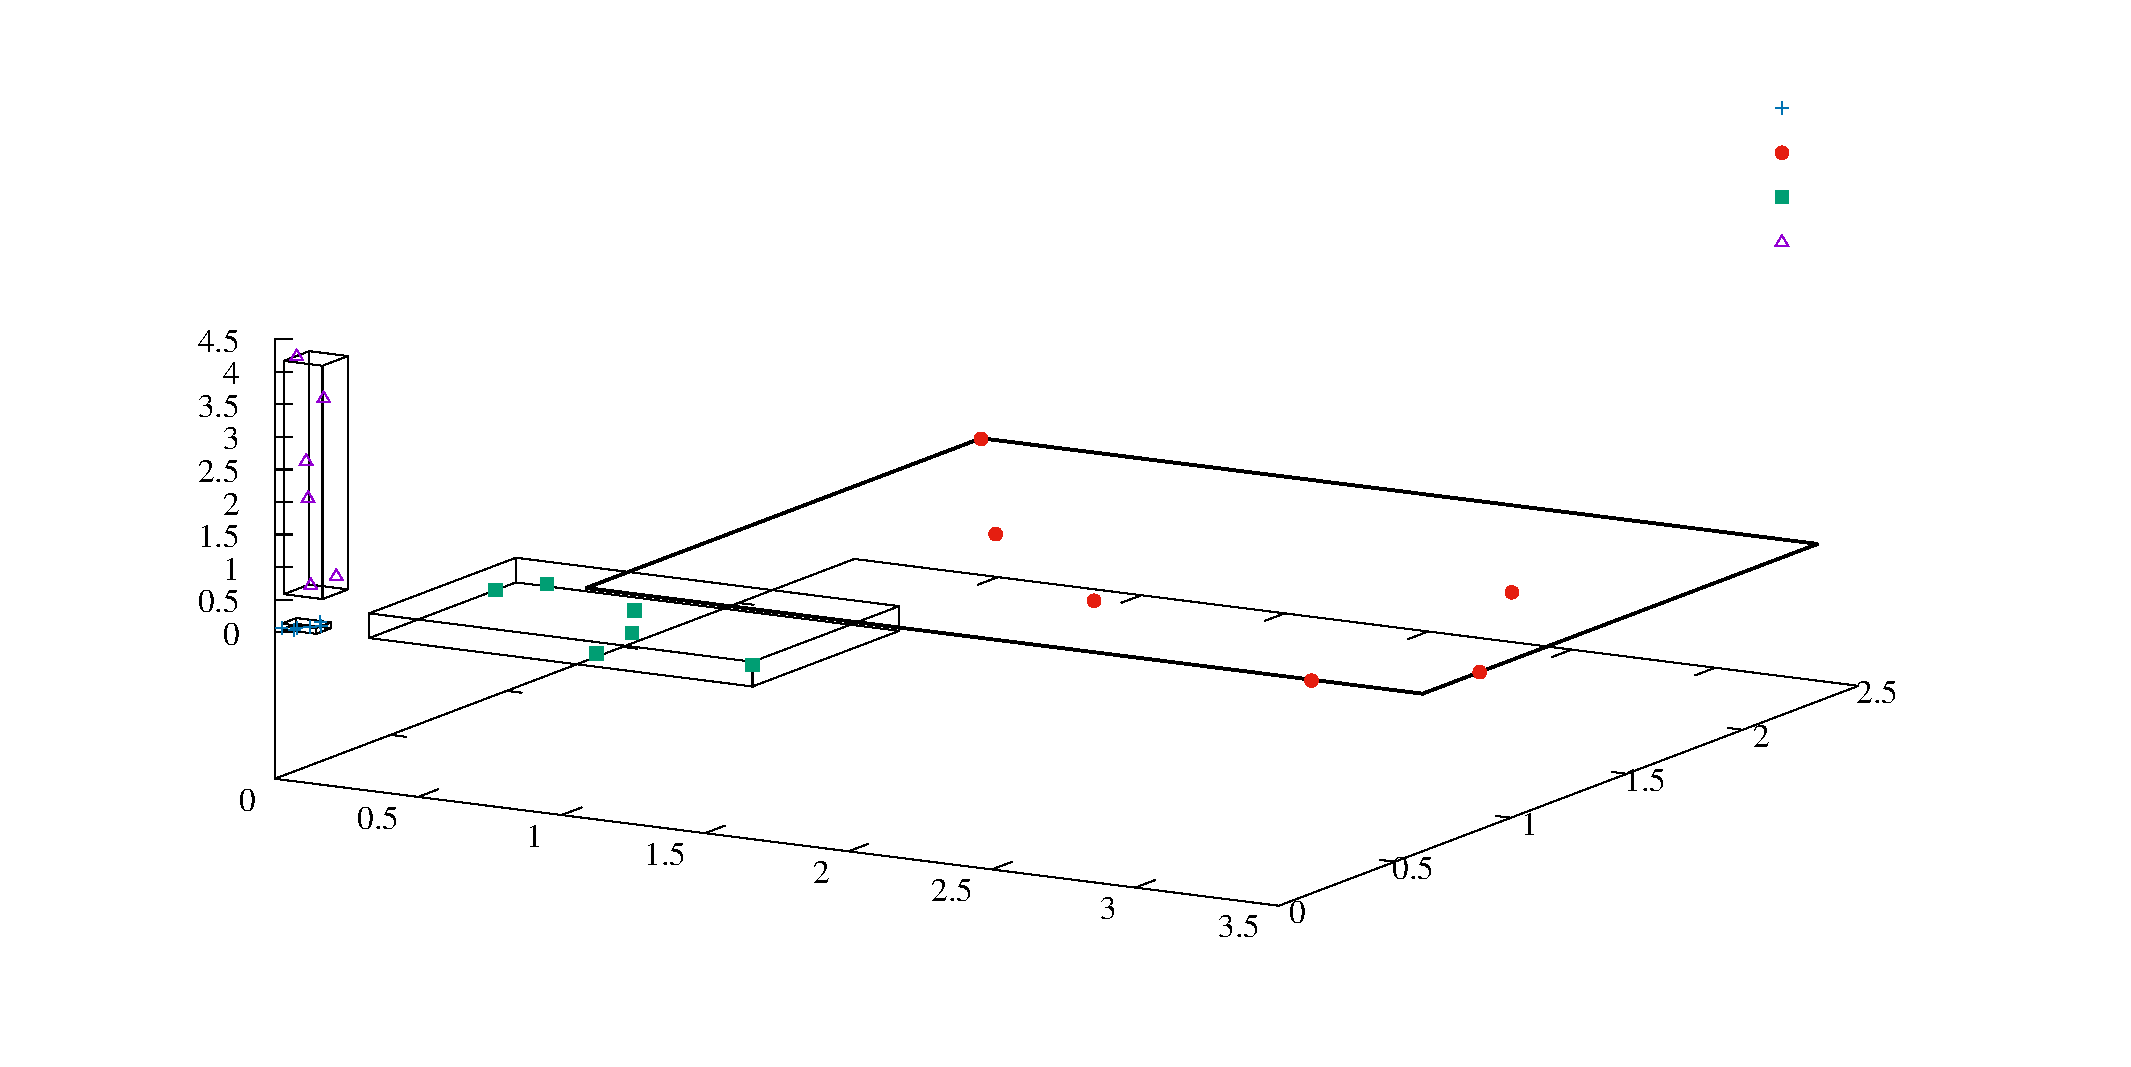
\includegraphics[scale=0.55]{Cajas.pdf}};
  \node at (-8.3,3) {\bf Regiones características de cada evento};
  \node[rotate=353] at (-11,-3.7) {Amplitud (0.066 Hz)};
  \node[rotate=20] at (-2.6,-3) {Amplitud (0.133 Hz)};
  \node[rotate=90] at (-16.4,-.5) {Amplitud (0.266 Hz)};
  \node at (-2,4) {\fontsize{8}{1}\selectfont Regular};
  \node at (-2.03,3.57) {\fontsize{8}{1}\selectfont Frenado};
  \node at (-2.01,3.15) {\fontsize{8}{1}\selectfont Rebase};
  \node at (-2,2.73) {\fontsize{8}{1}\selectfont Zig-zag};
\end{tikzpicture}
\end{textblock*}
\caption{Cada eje contiene los valores de las amplitudes para una de las tres frecuencias características.}
\label{Cajas}
\end{figure}

En la figura \ref{Cajas} se puede apreciar claramente la tendencia de los puntos de un mismo evento a agruparse en una determinada región.
Cada eje del espacio tridimensional corresponde a una de las frecuencias características de los eventos. 
Mientras que las coordenadas de cada eje representan la amplitud relativa a cada frecuencia. 
Según el valor de estas amplitudes, el punto en cuestión puede o no pertenecer a alguno de los eventos. 
Como se aprecia en la imagen existen diferentes zonas con forma de prisma, cada una de las cuales contiene puntos de determinado evento o de conducción regular. 
Dichos prismas dan una idea del espacio donde los valores de las amplitudes para un punto entran en la categoría de alguno de los tres eventos o de una conducción regular.
Estos prismas corresponden a las medidas de incertidumbre asociadas a cada una de las clases. 
Cada punto de la gráfica fue obtenido del espectro de frecuencias de ventanas que contenían muestras de datos de los eventos y conducciones regulares realizados.

Al hacer pasar la ventana de tiempo a la señal completa de un recorrido, se obtienen decenas de puntos como los de la figura \ref{Cajas}. 
Estos puntos se introducen como entrada del algoritmo antes mencionado, el cual como se mencionó consiste principalmente en una red neuronal que determina a qué tipo de evento pertenece la información de entrada.
Debido a que se usaron las funciones seno y coseno como funciones base para implementar la transformada de Fourier, existen dos puntos con información de frecuencias características para cada ventana de tiempo; uno relativo a las funciones seno y otro a las funciones coseno.
Por lo cual, se implementó el algoritmo de detección en tres modalidades distintas: en una se empleó la información de las frecuencias características relativas a las funciones coseno, en otra se hizo lo mismo con la información de las funciones seno, y en una tercera modalidad se intentó mejorar los resultados de detección de las dos anteriores, al establecer una función que utilice la información de las dos funciones armónicas.
Esta última modalidad solo consiste en multiplicar las componentes de la misma frecuencia de las salidas relativas a cada función armónica; con lo cual se genera un nuevo vector de salida al asignar cada uno de los tres productos a su componente correspondiente.
Este nuevo vector es el que se utiliza como salida para dicha modalidad.
Los resultados de la implementación de las tres modalidades del algoritmo se muestran a continuación (figuras de \ref{Deteccion_3_C.pdf} a \ref{Deteccion_5_CxS.pdf}):

\pagebreak
\ \\
\vspace{27cm}
\graficadeteccion{Deteccion_3_C.pdf}{de frenado}{cosenos}{Regular}{Rebase}{Zig-zag}{Frenado}{40mm}
\graficadeteccion{Deteccion_3_S.pdf}{de frenado}{senos}{Rebase}{Regular}{Zig-zag}{Frenado}{147mm}
\pagebreak
\ \\
\vspace{10.4cm}
\graficadeteccion{Deteccion_3_CxS.pdf}{de frenado}{producto de salidas}{Regular}{Rebase}{Frenado}{}{40mm}

\pagebreak
\ \\
\vspace{27cm}
\graficadeteccion{Deteccion_4_C.pdf}{de rebase}{cosenos}{Rebase}{Regular}{}{}{40mm}
\graficadeteccion{Deteccion_4_S.pdf}{de rebase}{senos}{Rebase}{Regular}{Zig-zag}{}{147mm}
\pagebreak
\ \\
\vspace{10.4cm}
\graficadeteccion{Deteccion_4_CxS.pdf}{de rebase}{producto de salidas}{Rebase}{Regular}{}{}{40mm}

\pagebreak
\ \\
\vspace{27cm}
\graficadeteccion{Deteccion_5_C.pdf}{de movimiento en zig-zag}{cosenos}{Rebase}{Regular}{Zig-zag}{}{40mm}
\graficadeteccion{Deteccion_5_S.pdf}{de movimiento en zig-zag}{senos}{Rebase}{Regular}{Zig-zag}{}{147mm}
\pagebreak
\ \\
\vspace{10.4cm}
\graficadeteccion{Deteccion_5_CxS.pdf}{de movimiento en zig-zag}{producto de salidas}{Rebase}{Regular}{Zig-zag}{}{40mm}

Después de analizar los resultados de detección de las tres modalidades, se decidió utilizar la tercera modalidad como parte del método de detección empleado para el último recorrido. 
Se realizó dicha elección debido a que, es la modalidad que presenta menor cantidad de errores en la detección de eventos anómalos y de conducciones regulares.

Complementariamente se presentan las gráficas de los valores de cada componente del vector de salida del algoritmo para cada ventana de tiempo (figuras de \ref{Salidas_3_C.pdf} a \ref{Salidas_5_CxS.pdf}).
Dichos valores concuerdan con las gráficas de detección.

\pagebreak
\ \\
\vspace{27cm}
\graficasalidas{Salidas_3_C.pdf}{Frenado}{Componente 1}{Componente 2}{Componente 3}{cosenos}{40mm}
\graficasalidas{Salidas_3_S.pdf}{Frenado}{Componente 1}{Componente 2}{Componente 3}{senos}{147mm}
\pagebreak
\ \\
\vspace{10.4cm}
\graficasalidas{Salidas_3_CxS.pdf}{Frenado}{Componente 1}{Componente 2}{Componente 3}{producto de salidas}{40mm}

\pagebreak
\ \\
\vspace{27cm}
\graficasalidas{Salidas_4_C.pdf}{Rebase}{Componente 1}{Componente 2}{Componente 3}{cosenos}{40mm}
\graficasalidas{Salidas_4_S.pdf}{Rebase}{Componente 1}{Componente 2}{Componente 3}{senos}{147mm}
\pagebreak
\ \\
\vspace{10.4cm}
\graficasalidas{Salidas_4_CxS.pdf}{Rebase}{Componente 1}{Componente 2}{Componente 3}{producto de salidas}{40mm}

\pagebreak
\ \\
\vspace{27cm}
\graficasalidas{Salidas_5_C.pdf}{Zig-zag}{Componente 1}{Componente 2}{Componente 3}{cosenos}{40mm}
\graficasalidas{Salidas_5_S.pdf}{Zig-zag}{Componente 1}{Componente 2}{Componente 3}{senos}{147mm}
\pagebreak
\ \\
\vspace{10.4cm}
\graficasalidas{Salidas_5_CxS.pdf}{Zig-zag}{Componente 1}{Componente 2}{Componente 3}{producto de salidas}{40mm}

\pagebreak

\section{Validación de la propuesta}

El último recorrido se realizó con la intención de validar los métodos de detección implementados en la sección anterior; motivo por lo cual, este recorrido no fue involucrado en la obtención de frecuencias características, ni ningún otro proceso de análisis; únicamente fue utilizado con fines de detección.
Durante el trayecto se ejecutaron los tres diferentes tipos de eventos, obteniendo los siguientes registros (figuras \ref{6x.pdf}, \ref{6y.pdf} y \ref{6z.pdf}):\zsavepos{registros}

\vspace{12.2cm}
\graficatreseventos{6x.pdf}{Recorrido para validación}{Zig-zag}{Frenado}{Rebase}{x}{\dimexpr\paperheight-\zposy{registros}sp+30mm}
\pagebreak
\ \\
\vspace{27cm}
\graficatreseventos{6y.pdf}{Recorrido para validación}{Zig-zag}{Frenado}{Rebase}{y}{40mm}
\graficatreseventos{6z.pdf}{Recorrido para validación}{Zig-zag}{Frenado}{Rebase}{z}{147mm}
\pagebreak

Observando la gráfica relacionada al eje $x$, se puede apreciar fácilmente el patrón característico del evento de frenado y con una amplitud menor, el pico generado por el evento de rebase. 
Como se ha visto anteriormente, el evento de frenado y rebase no tienen mucha relevancia sobre el eje $y$.
El evento de movimiento en zig-zag, al igual que en las demás gráficas del eje $x$ donde está presente, no tiene mucha notoriedad en esta dimensión, no así en el eje $y$, donde es el evento que se puede identificar con mayor facilidad. 
Por último, en lo que corresponde al eje $z$, ninguno de los eventos es diferenciable a simple vista de los demás.

De los resultados de detección obtenidos en la sección anterior para la tercera modalidad, se observó que, en la mayoría de los casos, en los primeros segundos de la realización de cada evento el algoritmo, este no es capaz de reconocer el evento en cuestión con un grado de eficiencia aceptable.
Esto es debido a que, en los primeros segundos de la realización de un evento, la ventana no contiene suficientes datos del evento para que en su espectro se obtengan valores relevantes, correspondientes a las frecuencias características.
Como consecuencia de esto, se obtiene una combinación de detección del eventos anómalos junto con varias detecciones de conducción regular; lo cual baja considerablemente la eficiencia en la detección.

Existen varios métodos para mejorar la detección durante el periodo mencionado, sin embargo, tales métodos requieren de herramientas teóricas de diferente temática a las aquí utilizadas; la forma implementar el algoritmo de detección al presente recorrido de validación se describe a continuación.

La ventana de detección recorre los intervalos etiquetados como conducción regular de principio a fin.
La eficiencia en la detección de una conducción regular se calcula dividiendo el número de veces que el algoritmo detectó una conducción regular en los intervalos de tiempo con esta etiqueta, entre el número total de ventanas presentes en dichos intervalos.

Para cualquiera de los tres eventos detectables, la ventana inicia su recorrido cinco segundos después de comenzar el evento y lo termina cuando el evento finaliza, por lo que se anula la detección durante los primeros cinco segundos a partir del inicio de un evento.
La eficiencia en la detección de los eventos se calcula de forma análoga a la de la conducción regular.

Los resultados de detección para este recorrido se presentan en las siguientes gráficas (figuras \ref{Deteccion_6_C.pdf}, \ref{Deteccion_6_S.pdf} y \ref{Deteccion_6_CxS.pdf}), en donde se muestran los resultados de las tres modalidades de detección, pero, como se mencionó anteriormente, la tercera modalidad es la que presenta menor cantidad de errores, por lo cual es la que se utilizará para el cálculo de la eficiencia en la detección.

\pagebreak
\ \\
\vspace{27cm}
\graficadeteccion{Deteccion_6_C.pdf}{para validación}{cosenos}{Regular}{Zig-zag}{Rebase}{Frenado}{40mm}
\graficadeteccion{Deteccion_6_S.pdf}{para validación}{senos}{Rebase}{Regular}{Zig-zag}{Frenado}{147mm}
\pagebreak
\ \\
\vspace{10.4cm}
\graficadeteccion{Deteccion_6_CxS.pdf}{para validación}{producto de salidas}{Regular}{Zig-zag}{Rebase}{Frenado}{40mm}

La información cuantitativa de la detección en el presente recorrido, con el método de detección anteriormente descrito, se presenta en la siguiente tabla:
%\diagbox[width=10em]{Diag\\Column Head I}{Diag Column\\Head II}

\begin{table}[H]
\centering
\begin{tabular}{||c|c|c|c|c||c||}
\hhline{|t:=====:t:=:t|}
\backslashbox{\bf Etiqueta\\ \\ }{\\ \bf Detectados} & \begin{sideways}\hspace{-0.7cm}Regular\end{sideways} & \begin{sideways}\hspace{-0.7cm}Frenado\end{sideways} & \begin{sideways}\hspace{-0.7cm}Rebase\end{sideways} & \begin{sideways}\hspace{-0.7cm}Zig-zag\end{sideways} & \begin{sideways}\hspace{-0.7cm}{\bf Eficiencia}\end{sideways} \\ 
\hhline{||-----||-||}
Regular & 127 & 3 & 20 & 10 & \bf 0.79 \\ 
\hhline{||-----||-||}
Frenado & 5 & 18 & 0 & 0 & \bf 0.78 \\ 
\hhline{||-----||-||}
Rebase & 4 & 0 & 15 & 0 & \bf 0.78 \\ 
\hhline{||-----||-||}
Zig-zag & 14 & 0 & 0 & 9 & \bf 0.39 \\ 
\hhline{|b:=====:b:=:b|}
\end{tabular}
\caption{Detecciones realizadas durante los intervalos relativos a cada evento e intervalos de conducción regular.}
\label{matriz}
\end{table}

En la tabla \ref{matriz} se puede apreciar que la eficiencia en la detección del movimiento en zig-zag es muy baja.
Esto es debido a que la forma de la señal sobre el eje $y$ cuando se ejecuta este evento es muy parecida a las funciones seno o coseno, para una frecuencia y amplitud particulares.
Por lo que cuando la señal contenida en la ventana está en fase con alguna de las dos funciones; esto dará como resultado que tal función tenga una contribución fuerte a dicha señal al realizar el análisis de Fourier, mientras que la otra función tendrá una amplitud pequeña en comparación al no estar en fase con la señal.
Es por ello que, al hacer el producto de las salidas de las funciones seno y coseno para llevar a cabo la detección, se obtiene un gran porcentaje de valores pequeños en la componente correspondiente al evento de movimiento en zig-zag. 
Razón por la cual se decidió implementar un segundo método de detección para tal evento.
Dicho método consiste simplemente en considerar como detección de un movimiento en zig-zag cuando cualquiera de las salidas del algoritmo para las funciones seno o coseno correspondan a un movimiento en zig-zag.

Los resultados del cambio en el método de detección para el evento de zig-zag se presentan en la siguiente gráfica:\zsavepos{grafica}

\vspace{12.2cm}
\graficadeteccion{Deteccion_6_CxS2.pdf}{para validación}{m{\'e}todo de detecci{\'o}n alternativo}{Regular}{Zig-zag}{Rebase}{Frenado}{\dimexpr\paperheight-\zposy{grafica}sp+10mm}

Al implementar este método, la eficiencia en la detección del movimiento en zig-zag aumenta considerablemente, como se puede apreciar en la siguiente tabla.

\begin{table}[H]
\centering
\begin{tabular}{||c|c|c|c|c||c||}
\hhline{|t:=====:t:=:t|}
\backslashbox{\bf Etiqueta\\ \\ }{\\ \bf Detectados} & \begin{sideways}\hspace{-0.7cm}Regular\end{sideways} & \begin{sideways}\hspace{-0.7cm}Frenado\end{sideways} & \begin{sideways}\hspace{-0.7cm}Rebase\end{sideways} & \begin{sideways}\hspace{-0.7cm}Zig-zag\end{sideways} & \begin{sideways}\hspace{-0.7cm}{\bf Eficiencia}\end{sideways} \\ 
\hhline{||-----||-||}
Regular & 115 & 3 & 20 & 22 & \bf 0.71 \\ 
\hhline{||-----||-||}
Frenado & 5 & 18 & 0 & 0 & \bf 0.78 \\ 
\hhline{||-----||-||}
Rebase & 3 & 0 & 15 & 1 & \bf 0.78 \\ 
\hhline{||-----||-||}
Zig-zag & 0 & 0 & 0 & 23 & \bf 1 \\ 
\hhline{|b:=====:b:=:b|}
\end{tabular}
\caption{Detecciones realizadas durante los intervalos relativos a cada evento e intervalos de conducción regular, implementando un método alternativo para la detección del movimiento en zig-zag.}
\end{table}

Como se puede apreciar en las gráficas de detección, tanto para los recorridos enfocados a un evento como en el recorrido para validación existen falsos positivos y negativos en la detección de los eventos.
Algunos de los cuales se pueden identificar como puntos aislados de un evento en un intervalo de conducción regular o de otro evento diferente, o como puntos de una conducción regular, en el intervalo correspondiente a un evento anómalo.
Se cree que esto sucede debido a la realización de diferentes movimientos durante los intervalos de conducción regular, los cuales, si bien son conservadores, no evitan que haya cambios de aceleración considerables sobre los distintos ejes.
Dentro de estos movimientos se encuentran el recorrer una curva o incorporar el vehículo al carril de tránsito, partiendo de una velocidad cero.
Otra de las causas es el parecido entre los eventos de frenado y rebase, los cuales poseen las mismas frecuencias características, lo que sumado a la poca cantidad de muestras que se dispone de cada evento para diferenciarlos entre sí (cuatro para cada uno), tiene como consecuencia que el algoritmo confunda en algunas situaciones a estos eventos.

Al igual que el problema de detección al inicio de un evento, existen técnicas para eliminar estos falsos positivos y negativos, las cuales requieren de métodos no relacionados al marco teórico con el que se pretende llevar a cabo el presente trabajo.
Por tal motivo no se abordará dicho problema en esta ocasión.

Complementariamente se presentan las gráficas de los valores de cada componente del vector de salida del algoritmo para cada ventana de tiempo (figuras de \ref{Salidas_6_C.pdf} a \ref{Salidas_6_CxS2.pdf}).

\pagebreak
\ \\
\vspace{27cm}
\graficasalidas{Salidas_6_C.pdf}{Recorrido para validación}{Componente 1}{Componente 2}{Componente 3}{senos}{40mm}
\graficasalidas{Salidas_6_S.pdf}{Recorrido para validación}{Componente 1}{Componente 2}{Componente 3}{cosenos}{147mm}
\pagebreak
\ \\
\vspace{27cm}
\graficasalidas{Salidas_6_CxS.pdf}{Recorrido para validación}{Componente 1}{Componente 2}{Componente 3}{producto de salidas}{40mm}
\graficasalidas{Salidas_6_CxS2.pdf}{Recorrido para validación}{Componente 1}{Componente 2}{Componente 3}{método de detección alternativo}{147mm}
\pagebreak

Después de analizar los resultados obtenidos hasta ahora, se ha determinado que los inconvenientes de mayor peso para la diferenciación y detección de estos tres eventos consisten en la discriminación automática de los eventos de frenado y rebase. 
Los cuales poseen las mismas frecuencias características en sus respectivos espectros. 
Estas frecuencias, en algunas ocasiones, no tienen la suficiente amplitud para diferenciarlas de una manera confiable de las amplitudes obtenidas en una conducción regular. 
Con respecto al evento de movimiento en zig-zag no se tienen este tipo de problemas ya que debido a sus características se puede discriminar fácilmente de los demás eventos.


% !TEX encoding = UTF-8 Unicode
\chapter{Conclusiones}\label{chap:conclusiones}
%
%
En el presente trabajo se diseñó un método para el acomodo de objetos en un espacio delimitado, el cual tiene como objetivo reducir el posterior costo de acceso a estos.
Para ello se abordó el problema de una forma simplificada de como se haría en una situación real.
Esto es, discretizando el espacio donde se colocan los objetos, así como reduciendo la complejidad geométrica de los objetos y la cantidad de clases u objetos distintos que se pueden utilizar.
Debido a su naturaleza discreta, el problema se puede abordar como una búsqueda en un espacio de permutaciones, para lo cual existen diversas metodologías y algoritmos de búsqueda, de entre los cuales se optó por un algoritmo de recocido simulado.

Dado que no existe a la fecha una investigación que aborde el problema planteado, el aporte principal del presente trabajo es la definición de los parámetros y reglas para evaluar qué tan adecuado es un acomodo, de acuerdo a los objetivos establecidos.
Dicha evaluación está basada en la geometría de los objetos y en cómo esta afecta su sujeción cuando los objetos están en determinada configuración.
De forma que al combinar esto con el algoritmo de búsqueda elegido, se puede obtener el acomodo requerido.

Los resultados muestran que, en los casos donde fue posible comparar el método propuesto con una búsqueda exhaustiva, se obtuvo en el 91.7\% de los casos, los mismos resultados que dicha búsqueda, esto es, un arreglo óptimo de acuerdo a las reglas establecidas.
Mientras que en casos más complejos, en los que no fue posible realizar una búsqueda exhaustiva, los resultados siguen siendo buenos, llegando a ser óptimos en varios casos para los que fue posible determinar tal característica.
Con lo cual, se puede aceptar la hipótesis de investigación propuesta, al menos para el problema definido.

Como trabajo futuro se propone expandir las capacidades del método desarrollado.
Esto es, adaptarlo para que se puedan abordar casos más complejos y diversos, por ejemplo, con una mayor cantidad de objetos, así como incluir más variedades de geometrías para estos, es decir, incluir una mayor cantidad de clases.
Además, se podrían relajar las restricciones acerca de cómo se pueden colocar los objetos en el espacio, permitiendo configuraciones en las que los objetos puedan ser colocados encima de otros y además puedan tener un número mayor de orientaciones.

El método de búsqueda también podría cambiar y mejorarse de acuerdo a estas expansiones.
Se podría implementar otra técnica de búsqueda, o bien, utilizar una combinación de estas para diseñar una metodología que se adapte de mejor manera al problema planteado.

%\appendix
%\include{apendiceA}
%\include{apendiceB}
%\include{apendiceC}
\let\chapter\oldchapter
%\renewcommand{\refname}{Bibliograf{\'i}­a}
\renewcommand\bibname{Referencias}
\lhead{\it Referencias}
\bibliographystyle{unsrt}
\bibliography{Bibliografia}
\addcontentsline{toc}{chapter}{Referencias}
\end{document}